\documentclass[aps,showpacs,twocolumn,
prd,superscriptaddress,nofootinbib]{revtex4-1}

\usepackage{amsmath}
\usepackage{amsfonts}
\usepackage{amssymb}
\usepackage{latexsym}
\usepackage{graphicx}
\usepackage{bm}
\usepackage{color}
\usepackage{enumerate}
\usepackage{ulem}
\usepackage{tabularx}

\usepackage{graphicx}
\usepackage[caption=false]{subfig}
%\usepackage{caption}
%\usepackage{subcaption}
%\captionsetup{compatibility=false}

\usepackage{color}
\usepackage[usenames,dvipsnames,svgnames,table]{xcolor}
%\usepackage[colorlinks=true,
%            linkcolor=green,
%            urlcolor=blue,
%            citecolor=red]{hyperref}
\usepackage[colorlinks=true,
            linkcolor=YellowOrange,
            urlcolor=RoyalBlue,
            citecolor=RedViolet]{hyperref}
            
%\usepackage{showlabels}

\newcommand{\be}{\begin{equation}}
\newcommand{\ee}{\end{equation}}
\newcommand\ud{{\mathrm{d}}}
\newcommand\uD{{\mathrm{D}}}
\newcommand\calO{{\mathcal{O}}}
\newcommand\calM{{\mathcal{M}}}
\newcommand\calF{{\mathcal{F}}}
\newcommand\calT{{\mathcal{T}}}
\newcommand\calD{{\mathcal{D}}}
\newcommand\calA{{\mathcal{A}}}
\newcommand\bfx{\mathbf{x}}
\newcommand{\ov}[1]{\overline{#1}}
\newcommand{\ph}[1]{\phantom{#1}}
\newcommand{\cte}{\mathrm{cte}}
\newcommand{\nn}{\nonumber}
%\newcommand{\hatk}{\hat{k}}
\newcommand{\hatk}{k}
\newcommand{\Hz}{\,\mathrm{Hz}}
\newcommand{\sinc}{\,\mathrm{sinc}}
\newcommand{\Msol}{M_{\odot}}
\newcommand{\tf}{t_{f}}
\newcommand{\Tf}{T_{f}}
\newcommand{\tfd}{t_{f}^{d}}
\newcommand{\tfSPA}{t_{f}^{\rm SPA}}

\newcolumntype{C}[1]{>{\centering\arraybackslash}p{#1}}
\newcolumntype{L}[1]{>{\raggedright\arraybackslash}p{#1}}

\newcommand{\SM}[1]{{\color{Red} #1}}
\newcommand{\jgb}[1]{{\color{DarkGreen} #1}}

\begin{document}

\title{Fourier-domain modulations and delays of gravitational-wave signals}

\author{Sylvain Marsat}
\affiliation{Max Planck Institute for Gravitational Physics (Albert Einstein Institute), Am M\"uhlenberg 1, Potsdam-Golm, 14476, Germany}
\author{John G. Baker}
\affiliation{Gravitational Astrophysics Laboratory, NASA Goddard Space Flight Center, 8800 Greenbelt Rd., Greenbelt, MD 20771, USA}
\affiliation{Joint Space-Science Institute, University of Maryland, College Park, MD 20742, USA}

\date{\today}

\begin{abstract}

We present a Fourier-domain based approach modulations and delays of gravitational wave signals, a problem which arises in two different contexts. For space-based detectors like LISA, the orbital motion of the detector introduces a time-dependency in the response of the detector, consisting of both a modulation and a varying delay. In the context of signals from precessing spinning binary systems, a useful tool for building models of the waveform consists in representing the signal as a time-dependent rotation of a quasi-non-precessing waveform. In both cases, being able to compute transfer functions for these effects directly in the Fourier domain may enable performance improvements for data analysis applications by using fast frequency-domain waveforms. Our results generalize previous approaches based on the stationary phase approximation, extending them by including delays and higher-order corrections while being applicable to a broader class of signals including full inspiral-merger-ringdown waveforms. In the LISA case, we find that higher-order corrections remain small except at the two extremes of the detector's frequency band, where we show that including them reduces the errors. In the case of precessing binaries, we perform a limited exploration of the merger-ringdown range based on a toy model for the precession. We find that, depending on the post-merger frame velocity, higher-order corrections can become quantitatively large to the point of challenging our perturbative formalism, while affecting mainly the amplitude and giving rise to limited unfaithfulness. We further present an alternative direct convolution approach to accurately represent these post-merger features.

\end{abstract}

\pacs{
04.25.D-, % numerical relativity
04.70.Bw, % classical black holes
04.80.Nn, % Gravitational wave detectors and experiments
95.30.Sf, % relativity and gravitation
95.55.Ym, % Gravitational radiation detectors
97.60.Lf  % black holes (astrophysics)
}

\maketitle

%%%%%%%%%%%%%%%%%%%%%%%%%%%%%%%%%%%%
%%%%%%%%%%%%%%%%%%%%%%%%%%%%%%%%%%%%

\section{Introduction}
\label{sec:intro}

With the recent detections of gravitational-wave signals emitted by the coalescences of binary black holes, announced by the LVC collaboration during the first and second obervation runs of the two LIGO instruments~\cite{LIGO-theevent-2016,LIGO-christmasevent-2016,LIGO-O1BBH-2016}\jgb{[update refs]}, gravitational-wave astronomy has entered its observational era. With the conclusion of LIGO's second observation run, and the recent extension of the ground-based detectors network with Virgo~\cite{Virgo} ( and later also KAGRA~\cite{KAGRA} and LIGO-India~\cite{INDIGO}), many more detections from compact object coalescences are to come, with binary black holes being expected to be the dominant sources~\cite{} \SM{[C]}.

Moreover, the European Space Agency has issued a mission call \SM{[update]} for its L3 space mission with a tentative launch around 2034, adressing the science theme ``The Gravitational Universe'', possibly opening the way for a space-borne observatory based on the concept of the Laser Interferometer Space Antenna (LISA)~\cite{LISA09,LISA17}. Among other sources of gravitational waves, LISA will be able to detect and characterize comparable-mass binary black hole coalescences to cosmological distances over a wide range of masses, from high-redshift observations of supermassive black hole binaries with $M\sim 10^{7} \Msol$ down to the observation of LIGO-type sources with $M\sim 10^{2} \Msol$~\cite{Sesana16}.

Data analysis for gravitational-wave observations of compact binary coalescences require accurate models (or templates) for the signals, both for ensuring efficient detections of signals that may be buried in instrumental noise, and to extract the physical parameters of the source in a subsequent analysis. The the greater sensitivity of LISA and other future instruments will require further increases in the accuracy of computationally efficient signal templates. This motivates an important and ongoing effort to improve gravitational wave templates. Two important focus areas for template improvements are need to cover all phases of the evolution of the system, including the inspiral, merger and ringdown (IMR), which became possible thanks to the breakthrough of numerical relativity~\cite{Pretorius05,Baker+06,Campanelli+06}, and the inclusion of the effects of the spins of the compact objects, that can lead to a precession of the orbital plane~\cite{ACST94,K95}. Besides accuracy, the computational efficiency of template generation is crucial. Bayesian analysis for parameter estimation of gravitational-wave signals, as was performed for the LIGO detections~\cite{LIGO-theeventPE-2016,LIGO-O1BBH-2016}, may require millions of evaluations of the likelihood function to sample the posterior probability distribution. \SM{[objective: accuracy, not necessary necessary for LIGO now but in the future yes]}

The GW community is making progress assembling higher-fidelity tools for these coming challenges.
State-of-the-art IMR templates combine information from the perturbative results of post-Newtonian theory covering the inspiral (see e.g.~\cite{BlanchetLiving}) and from numerical relativity simulations covering the end of the inspiral and the merger-ringdown phase (see e.g.~\cite{Pfeiffer12}). The Effective-One-Body (EOB) approach~\cite{BD99} does so by incorporating a resummation of post-Newtonian results and a calibration to numerical relativity, and has been extended to include both spins of the two bodies~\cite{Taracchini+13, Pan+13, Bohe+16}. Phenomenological templates extend post-Newtonian models by postulating an analytic ansatz for the Fourier-domain amplitude and phase, fitting coefficients against numerical relativity waveforms~\cite{Husa+15, Khan+15}, and can include a simplified model for precession~\cite{Hannam+13}. The second type of models produce directly the amplitude and the phase of the Fourier-domain waveform components in the form of a piecewise analytic function. EOB waveforms, by contrast, require integration of ordinary differential equations in the time-domain, which can be time-consuming. For the non-precessing case, Reduced Order Models (ROM), also called surrogate models, have been developed to speed up considerably the waveform generation, without losing accuracy~\cite{Field+13, Puerrer14, Bohe+16}. Both approaches are therefore able to efficiently produce IMR Fourier-domain waveforms. An important aspect is that the resulting waveforms can be represented by an amplitude and phase for each mode, with only a few hundred samples~\cite{Puerrer14}.

A complete representation of spin effects in fast IMR templates still remains a frontier of gravitational wave signal modelling. In presence of misaligned spins, the system will endure precession of the orbital plane as it evolves, leading to modulations of the signal as seen by the observer~\cite{ACST94}. Precessing EOB templates incorporate all six parameters of the two spins~\cite{Pan+13, BTB16} but still require a costly time-domain integration; while precessing phenomenological templates~\cite{Hannam+13} decrease the dimensionnality by using effective spin parameters representing only the dominant effects of the spins. To model the effect of precession on the emitted waveform, it has been proposed~\cite{BCV03b, BCPTV05, Schmidt+10, OShaughnessy+11, Boyle+11} to decompose precessing waveforms by performing a time-dependent rotation, following the precession of the orbital plane. The resulting waveform in the rotated frame can then be modelled by a non-precessing waveform, an approximation which is used both in the construction of the inspiral part of precessing EOB waveforms~\cite{Pan+13} and in the construction of precessing phenomenological waveforms~\cite{Hannam+13}. To follow this modelling approach and efficiently create Fourier-domain waveforms, one needs to understand how to translate the time-domain modulations created by the frame rotation into a Fourier-domain transfer function, which is our first motivation.

Prospective parameter recovery studies for LISA observations of comparable-mass binary black hole coalescences aim at characterizing the scientific performance of the future experiment. Although LISA~\cite{LISA17} is still at least a decade from launch, the ESA L3 mission is rapidly progressing into its early stages where mission design choices must be informed by science impact analysis. However, the recent progresses in waveform modelling, most notably the availability of fast and accurate IMR waveforms, have not yet made their way to the field of LISA data analysis studies. In the past, many such studies used post-Newtonian, inspiral-only models, and were limited to the cheaper Fisher-matrix formalism instead of a full Bayesian analysis (among numerous works, see e.g. \cite{Cutler97,LISAPE09}). Refs.~\cite{McWilliams+09,McWilliams+10,McWilliams+11} explored the effects of including the merger and ringdown, keeping the mass parameters fixed. However, the Fisher matrix analysis, although considerably cheaper to perform, is valid only in the limit of a high signal to noise ratio (SNR). Several implementations of Bayesian analyses were developed~\cite{CP06,Wickham+06,Babak+08,GP09,Feroz+09,Petiteau+10,PC13} (see also~\cite{MLDC4} and references therein), with Ref.~\cite{PC15} proposing a direct comparison of Fisher and Bayes analyses, but they were limited to inspiral-only waveforms. One exception was Ref.~\cite{Babak+08} where IMR signals were used in a Bayesian study, but there the masses of the black holes were kept fixed. In the recent Ref.~\cite{Klein+15}, the limitation to inspiral-only precessing post-Newtonian waveforms was compensated by an SNR reweighting procedure. Thus, due mainly to their high computational cost, full-fledged Bayesian parameter estimation simulations for IMR signals are still missing. \jgb{[Maybe there is too much detail in this paragraph?]}

%Prospective parameter recovery studies for LISA observations of comparable-mass binary black hole coalescences aim at characterizing the scientific performance of the future experiment. Although LISA~\cite{LISA17} is still at least a decade from launch, the ESA L3 mission is rapidly progressing into its early stages where mission design choice must be informed by science impact analysis. However, the recent progresses in waveform modelling, most notably the availability of cheap IMR waveforms, have not yet made their way to the field of LISA data analysis studies. In the past, such studies used mainly post-Newtonian, inspiral-only models, and were limited to the Fisher-matrix formalism instead of full Bayesian analysis (among numerous works, see e.g. \cite{Cutler97,LISAPE09}). Refs.~\cite{McWilliams+09,McWilliams+10,McWilliams+11} explored the effects of including the merger and ringdown, keeping the mass parameters fixed. However, the Fisher matrix analysis, although considerably cheaper to perform, is valid only in the limit of a high signal to noise ratio (SNR) and has known shortcomings~\cite{Vallisneri08}. Several implementations of Bayesian analyses were developed~\cite{CP06,Wickham+06,Babak+08,GP09,Feroz+09,Petiteau+10,PC13} (see also~\cite{MLDC4} and references therein), with Ref.~\cite{PC15} proposing a direct comparison of Fisher and Bayes analyses, but they were limited to inspiral-only waveforms. One exception was Ref.~\cite{Babak+08} where IMR signals were used in a Bayesian study, but there the masses of the black holes were kept fixed. In the recent Ref.~\cite{Klein+15}, the limitation to inspiral-only precessing post-Newtonian waveforms was compensated by an SNR reweighting procedure. Thus, due mainly to their high computational cost, full-fledged Bayesian parameter estimation simulations for IMR signals are still missing. \jgb{[Maybe there is too much detail in this paragraph?]}

In contrast with current ground-based detectors, which are typically sensitive to chirping binaries for less than a second, LISA signals may accumulating over months or years.
The response of a LISA-type instrument is thus time-dependent~\cite{Cutler97}.
The motion and change of orientation of the detector constellation along its orbit lead to significant time variability in the form of a modulation and a varying delay. These effeccts then convey information about the localization of the gravitational-wave source in the sky. The complicated detector response increase the computational cost of parameter-estimation analyses. To leverage the performance of state-of-the-art Fourier-domain IMR templates~\cite{BTB16,Khan+15}, one needs to be able to process the signals through the time-dependent response of the dectector while staying in the Fourier domain.

The purpose of this paper is to introduce a formalism for efficiently processing signals through a time-domain modulation and delay within the Fourier domain, while retaining the compactness of a Fourier-domain amplitude and phase representation of the signals. This will allow us to address both the issue of the Fourier-domain response of the LISA instrument, as well as the issue of Fourier-domain precession modulation for IMR signals from precessing binaries.

In previous works, the Stationary Phase Approximation (SPA) (see e.g.~\cite{Thorne300, CF94}) has been often used for this purpose. The SPA is a common approximation to compute the Fourier transform of non-precessing signals during the inspiralling phase. In the case of precessing binaries, applying it directly to the modulated signal is however prone to pathologies. In Ref.~\cite{KCY13,KCY14}, a formalism (called shifted uniform asymptotics or SUA) was introduced to go beyond the SPA and compute more accurately the modulation in the Fourier domain; however, this formalism still relies on the SPA for the underlying precessing-frame signal, and is as such limited to inspiralling signals. Another intuitive approach consists in using a time-to-frequency correspondence, such as the one given by the SPA, to directly carry over the modulation to the Fourier domain. This corresponds, in a sense to be detailed below, to the zeroth-order approximation of the SUA, and it is used implicitly\footnote{With the difference that the expressions used for the modulation are given in terms of frequency directly for the inspiral, and are then extended to also cover high frequencies in the merger-ringdown part of the signal, as we will discuss below.} for the simplified precession of the phenomenological waveforms of Ref.~\cite{Hannam+13}. In the case of the LISA response, the SPA provides a natural map from time-domain (for the orbit) to Fourier-domain (for the signal)~\cite{Cutler97}. Ref.~\cite{Klein+15} included the orbital motion of the detector in the SUA treatment. Consistently extending these previous approaches to the merger-ringdown part of the signals, including the delays in the LISA case, is part of the objectives of this paper.

The plan of the paper is as follows. In Sec.~\ref{sec:motivation}, we motivate the problem of Fourier-domain modulation and introduce the relevant timescales for both the response of LISA-type detectors and the modulation of precessing signals. In Sec.~\ref{sec:formalism}, we present our general formalism, give its leading order approximation as well as higher-order corrections, introduce new timescales based on the Fourier-domain signal, refine the previous results for both the quadratic-in-phase corrections and the treatment of the delays, and make the connection to previous approaches of the problem. We then apply our formalism to the response of the LISA detector in Sec.~\ref{sec:LISA}, and to the case of signals from precessing binaries in Sec~\ref{sec:precession}. We discuss and summarize our results in Sec.~\ref{sec:discussion}.

%%%%%%%%%%%%%%%%%%%%%%%%%%%%%%%%%%%%
%%%%%%%%%%%%%%%%%%%%%%%%%%%%%%%%%%%%

\section{Motivation}
\label{sec:motivation}

%%%%%%%%%%%%%%%%%%%%%%%%%%%%%%%%%%%%

\subsection{Basic considerations}
\label{subsec:basic}

We can jointly consider challenges in the contexts of both the LISA response and GW precession applications in terms of a more general problem which covers both domains. In each case must determine the Fourier transform of a signal $h(t)$ to which we apply a varying delay $d(t)$ before multiplication by a modulation function $F(t)$,
\be
\label{eq:delay-mod-defs}
	h_{d}(t) = h(t+d(t)) \,, \quad s(t) = F(t)h_{d}(t) \,,
\ee
and seek an efficient way to commpute the Fourier transform $\tilde{s}(f)$, expressed by means of a Fourier-domain transfer function $\calT$ such that
\be\label{eq:deftransfer}
	\tilde{s}(f) \equiv \calT(f) \tilde{h}(f) \,. 
\ee
As is well known, GW signals decomposed in spin-weighted spherical harmonic components are smoothly varying functions of frequency in amplitude/phase form. An important consequence is that these signal components can be accurately represented in terms of a relatively coarsely sampled frequency grid. This property will also extend to the transfer functions, allowing us to keep a compact representation of the full signals. (See Appendix~\ref{app:notation} for details of our notation and conventions for Fourier transforms and spherical harmonics.)

In the case of precessing binaries, the delays will be absent and the modulation functions will be the time-dependent Wigner coefficients applied to rotate the waveform from a precessing frame, where it verifies a restored mode hierarchy, to an inertial frame where the observations take place. In the case of a LISA-type detector, the signal $h(t)$ will simply be the waveform in a fixed heliocentric frame, and the delays will come from the motion of each detector in the wave front, while the modulation will represent the time-variation in the detector orientation.

In full generality computing the transfer function $\calT(f)$ would require a convolution, a costly (discretized) integral over the full frequency domain for each value of $f$. For our context though, there are some properties of $h(t)$, $d(t)$ and $F(t)$ which we can exploit for a more efficient computation. In particular, we will be able to exploit the separation of the different timescales in the problem.

First, the gravitational waveforms present a clear separation between the timescales of orbital motion and radiation-reaction. This leads to a general feature of GW signals from compact binaries, during the inspiral phase but also for black hole mergers, that the signal is relatively localized in time-frequency. The localization is particularly clear during the inspiral phase, where the SPA (see Sec.~\ref{subsec:SPA} below) provides an unambiguous time-to-frequency correspondence, however we will find that the applicability of the SPA will not be a limiting factor of our approach.

Second, the delay and modulation functions we consider are much more slowly varying than the GW signal. The relevant timescales are either the precession timescale for precessing binaries or the fixed annual-orbital motion timescale for the LISA response. This means that the modulation and delay have relatively compact support in the Fourier domain, hence the convolution with the signal will be localized in frequency, which justifies writing its output as a transfer function as in~\eqref{eq:deftransfer}.

Together, these observations let us think that, for a given $f$, only a limited range of times should be relevant in $d(t)$ and $F(t)$ so that we may expect to find a treatment for the transfer function that would be local in time for the modulation and delay. Intuitively, for an inspiral signal and in the limit of an extremely slowly varying $d(t)$ and $F(t)$, we should be able to simply evaluate them at the time given by the time-to-frequency correspondence of the SPA. Furthermore, a natural quantitative criterion for the applicability of this idea is given by the comparison of the radiation-reaction timescale of the signal with the modulation timescale (possibly augmented by a dimensionless factor when delays are present). In other words, the change in frequency of the signal over a characeteristic time of the modulation should be small for the separation of timescales to work.

Our objective is to find an approximate treatment for $\calT(f)$ which allows us to exploit these properties without relying on unnecessary limiting assumptions for the signal (like the limitation of the SPA to inspiral signals), which is extensible to the high-accuracies which will be required by LISA and other future gravitational-wave instruments, while being computationally efficient and widely applicable to GW analysis. Before introducing developing our formalism, though, we review the salient features of our application problems.

\subsection{Instrumental modulations and delays for LISA-type detectors}
\label{subsec:modulationLISA}

The response of a detector of the LISA type to an incident gravitational wave can be written in two different, equivalent forms, in terms of phase or frequency measurements. Here we will work with the second representation, which will prove more convenient for our purposes. Moreover, various notation and conventions have been used in the literature to label the spacecrafts and describe their orbits. We refer the reader to~\cite{Vallisneri04} for a comparative account on these various conventions. In this work, we will keep close to the conventions of~\cite{Vallisneri04}, which were also used in the Mock LISA Data Challenges (MLDC)~\cite{MLDC4}.

We use a coordinate system centered on the solar system barycenter (SSB), and we denote the center of the constellation by $O$. We introduce the notation $\hatk$ for the propagation vector of the gravitational wave, which we denote by $h_{ij}^{\rm TT}(t)$ in transverse-traceless matrix form, as measured at the SSB (thus, at position $p$, $h_{ij}^{\rm TT}(t, p) = h_{ij}^{\rm TT}(t - \hatk \cdot p)$). We denote by $p_{A}$ ($A=1,2,3$) the position of the spacecrafts and $n_{l}$ the unit vectors of the three links, with the convention that $n_{3}$ points from 1 to 2.

Written in terms of the fractional laser frequency shifts between two spacecrafts, the elementary response of the detector reads~\cite{EW75, RCP04, Vallisneri04}
\begin{align}\label{eq:yslr}
	y_{slr} &\equiv \frac{\nu_{r} - \nu_{s}}{\nu} \nn\\
	&= \frac{1}{2} \frac{n_{l}^{i}n_{l}^{j}}{1 - \hatk\cdot n_{l}} \left[ h_{ij}^{\rm TT}(t - L - \hatk\cdot p_{s}) - h_{ij}^{\rm TT}(t - \hatk\cdot p_{r}) \right] \,.
\end{align}
As detailed below in Sec.~\ref{}, we will use a rigid instantaneous model, approximating the geometry of the constellation by a moving equilateral triangle (neglecting the flexing of the arms induced by corrections in the orbits), and evaluating all geometric factors in~\eqref{eq:yslr} at a single time $t$ (neglecting pointing-ahead corrections). The additional delay $L$ (we use $c=1$) in the first term represents the light propagation time along the arm between spacecrafts $s$ and $l$.

The first- and second-generation TDI observables are then built as combinations of these basic building blocks, evaluated at delayed times. Since in our rigid approximation these delays will take a simple form in Fourier domain, we will focus in this paper on the $y_{slr}$ observables. We will give in Sec.~\ref{subsec:modelLISA} more details on the response of LISA-type detectors, on the TDI observables, and on the approximations that enter the derivation of the basic response~\eqref{eq:yslr} above.

The structure of~\eqref{eq:yslr} is such that one can build the full signal from individual contributions of the form
\be
	s(t) = F(t) h(t + d(t)) \,.
\ee
Here, $h(t)$ represents one of the individual modes building the full gravitational wave signal (see Eq.~\eqref{eq:defmodes}), $d(t)$ represents the time-varying delays of the form $-\hatk\cdot p_{A}(t)$, and $F(t)$ incorporates all the relevant geometric prefactors.

The functions $F(t)$ and $d(t)$ vary on a timescale of one year. When neglecting small non-periodic orbital perturbations (such as those caused by the influence of the Earth and of the other planets on the orbits), both $F(t)$ and $d(t)$ are periodic. It will also be useful to separate the delays in two types of terms: the first, $d_{O} = -\hatk\cdot p_{O}$, relates the waveform at the SSB to the waveform at the center of the constellation $O$, whereas the second, $d_{c}$, represents the various delays between the spacecrafts of the constellation. For an orbit radius $R=1\,\mathrm{au}$ and an armlength $L=2.5\times10^{6}\mathrm{km}$~\cite{LISA17}, $d_{O} \sim R/c \simeq 500\mathrm{s}$ and $d_{c} \sim L/c \simeq 8\mathrm{s}$.

%%%%%%%%%%%%%%%%%%%%%%%%%%%%%%%%%%%%

\subsection{Precession modulation for spinning binaries}
\label{subsec:modulationPrec}

For spinning compact objects, the presence of the spins leads to the precession of the orbit~\cite{Apostolatos+94, Kidder95}, which can have large effects on the waveform. In particular, it breaks the planar symmetry of the gravitational wave emission, and leads to modulations that are especially important for systems that are observed edge-on.

It was suggested by a number of authors~\cite{BCV03b, BCPTV05, Schmidt+10, OShaughnessy+11, Boyle+11} that the effect of the precession can be modeled, to a good approximation, by a time-dependent rotation of a non-precessing waveform. This allows for a modelling approach where one models separately a precessing frame following the evolution of the plane of the orbit, and approximates the waveform in this precessing frame by using a non-precessing model. Different prescriptions have been proposed for the construction of a precessing frame from the waveform itself~\cite{Schmidt+10, OShaughnessy+11, Boyle+11}.

If $(\alpha, \beta, \gamma)$ are the Euler angles relating the precessing frame to the inertial frame in the $(z,y,z)$ convention, the modes in the inertial frame $h_{\ell m}^{\rm I}$ are then related to the modes in the precessing frame $h_{\ell m}^{\rm P}$ by~\cite{Goldberg+67}
\be\label{eq:wignerrotintro}
	h_{\ell m}^{\rm I} = \sum\limits_{m=-\ell}^{\ell} \calD^{\ell *}_{mm'} (\alpha,\beta,\gamma) h_{\ell m'}^{\rm P} \,,
\ee
where the $\calD^{\ell}_{mm'}$ are Wigner matrices~\cite{} \SM{[C]}. Notice that there is no mixing of the modes with different values of $\ell$.

If we make the assumption that the precessing-frame waveform $h^{\rm P}$ is approximated by a non-precessing model that provides us with a smooth Fourier-domain amplitude and phase, then the problem reduces to computing the Fourier transform of the signal
\be\label{eq:defmodulationprec}
	s(t) = F(t) h(t) \,,
\ee
where the modulation function $F(t)$ is given by a Wigner matrix and depends on time through the Euler angles $(\alpha, \beta, \gamma)(t)$. We will discuss more in Sec.~\ref{subsec:modelPrec} \SM{[R]} the limitations of the assumptions used to perform the decomposition above.

In Eq.~\eqref{eq:defmodulationprec} above, the modulation function $F$ has time variations on the precessional timescale, which evolves throughout the inspiral. The separation between the precessional timescale and the orbital timescale will be crucial for our analysis. In the limit of low frequencies, we will see in Sec.~\ref{} \SM{[R]} below that, although these timescales become more and more separated, the decrease in the chirping rate gives raise to a corrective contribution that does not vanish in this limit. In the other limit, as the system gets close to merger, the separation of timescales becomes weaker, and we will explore in Sec.~\ref{} \SM{[R]} the application of our formalism to the merger and ringdown phase.

%%%%%%%%%%%%%%%%%%%%%%%%%%%%%%%%%%%%

\subsection{Stationary phase approximation}
\label{subsec:SPA}

As a preliminary step, we recall here an approximation widely used for similar purposes in treating gravitational waves signals emitted by inspiralling binaries, the Stationary Phase Approximation (thereafter SPA, and also sometimes called the steepest-descent method). It applies in general to chirping signals, and we refer the reader to~\ref{} for details. One first writes the time-domain signal in amplitude and phase form as $h(t) = a(t) e^{-2i\varphi(t)}$, where for gravitational wave signals $\varphi$ will correspond to the orbital phase, with the orbital frequency being $\omega = \dot{\varphi}$. In order to keep close to the notation used in the gravitational wave literature, we introduced a factor of 2 in the phase of the wave, which is appropriate for the dominant 22 harmonic of the signal. The approximation then applies to signals verifying the conditions \SM{[say that the third is sometimes missing ?]} \SM{[add reference to Finn-Chernoff, Cutler-Flanagan where the third one is missing]}
\be\label{eq:conditionsSPA}
	\left| \frac{\dot{a}/a}{\omega} \right| \ll 1\,, \quad \left|\frac{\dot{\omega}}{\omega^{2}} \right| \ll 1\,, \quad \left| \frac{(\dot{a}/a)^{2}}{\dot{\omega}} \right| \ll 1 \,.
\ee
Since the integral~\eqref{eq:defFT} defining the Fourier transform is rapidly oscillatory unless the term $2\pi f t$ cancels the evolution of $-2\varphi(t)$, its support is well centered around the point of stationary phase. This determines the time-to-frequency correspondence in the stationary phase approximation, and leads to the definition of this time as an implicit function of frequency by the relation
\be\label{eq:deftfSPA}
	\omega(\tfSPA) = \pi  f \,.
\ee
For a chirping signal of increasing phase, $\omega>0$ and $\dot{\omega}>0$, there is a unique point of stationary phase, located in the positive frequency range $f>0$. Using the conditions above, one can formally expand the signal around $\tfSPA$ to quadratic order in time, according to
\begin{align}
	\tilde{h}_{\rm SPA} (f) &\simeq a(\tfSPA) \exp\left[2i\pi f \tfSPA-2i\varphi(\tfSPA) \right] \nn\\
	& \qquad \cdot \int \ud t \, e^{-i \dot{\omega} (\tfSPA) (t-\tfSPA)^{2}} \,.
\end{align}
Note that to be able to treat the amplitude as a constant in the integral above, we used the third condition in~\eqref{eq:conditionSPA}. The resulting complex Gaussian integral yields\footnote{Note that the expressions given here are valid for the dominant mode $h_{22}$ of the waveform. They can be readily generalized to other modes $h_{\ell m}$ with phase $e^{-im\varphi}$.}
\begin{subequations}
\begin{align}
	\tilde{h}_{\rm SPA}(f) &= A_{\rm SPA}(f) e^{-i\Psi_{\rm SPA}(f)} \,, \\
	A_{\rm SPA}(f) &= a(\tfSPA) \sqrt{\frac{\pi}{\dot{\omega}(\tfSPA)}} \,, \\
	\Psi_{\rm SPA}(f) &= 2\varphi(\tfSPA) - 2\pi f \tfSPA + \frac{\pi}{4} \,. \label{eq:PsiSPA}
\end{align}
\end{subequations}
Ref.~\cite{Droz+99} evaluated the first correction to this approximation, within the context of post-Newtonian signals, and found that it can be considered as a term of the fifth post-Newtonian order, beyond the accuracy level of our current best models~\cite{BlanchetLiving}.

To understand the separation of timescales in the problem, it will be useful to have at hand the leading-order scaling laws for an inspiral (at the Newtonian order in the PN language). Although inaccurate for the purpose of waveform modelling, these Newtonian estimates will give useful orders of magnitude of the relevant timescales in the inspiral. For a binary with masses $m_{1}, m_{2}$, we define the total mass $M=m_{1}+m_{2}$ and the symmetric mass ratio $\nu = m_{1}m_{2}/M^{2}$. Introducing a time of coalescence $t_{c}$, the relations between the orbital frequency and phase and the time to coalescence $t_{c} - t$ are then given by
\begin{subequations}\label{eq:omegaphiN}
\begin{align}
	\omega(t) &= \left[ \frac{256\nu}{5c^{5}} (GM)^{5/3} (t_{c}-t) \right]^{-3/8} \,, \\
	\varphi(t) &= -\left[ \frac{c^{3}}{5 G M \nu^{3/5}} (t_{c}-t) \right]^{5/8} \,.
\end{align}
\end{subequations}
As for the leading-order time-domain amplitude of the $22$ mode, we have~\cite{BlanchetLiving}
\be\label{eq:a22N}
	a_{22}^{\rm N} (t) = \frac{2 G M \nu x}{D c^{2}} \sqrt{\frac{16 \pi}{5}} \,,
\ee
where we set $x = (G M\omega/c^{3})^{2/3}$ and where $D$ is the luminosity distance to the observer. For this Newtonian inspiral, applying the SPA gives for the $22$ mode $\tilde{h}(f) = A_{\rm N}(f)e^{-i\Psi_{\rm N}(f)}$ with
\begin{subequations}\label{eq:SPAN}
\begin{align}
	A_{N}(f) &= \frac{G^{2}M^{2} \pi}{Dc^{5}} \sqrt{\frac{2\nu}{3}} v^{-7/2}\,, \label{eq:ASPAN}\\
	\Psi_{\rm SPA}^{\rm N}(f) &= \phi_{0} - 2\pi f t_{0} - \frac{3}{128\nu v^{5}} \,, \label{eq:PsiSPAN} 
\end{align}
\end{subequations}
where we used the notation $v=(G M \pi f/c^{3})^{1/3}$ ($x=v^{2}$ with the SPA correspondence~\eqref{eq:deftfSPA}), and where $t_{0}, \phi_{0}$ are constants. It is also customary to rewrite the above relations in terms of the chirp mass $\calM \equiv M\nu^{3/5}$, which is the only mass combination characterizing the signal at the leading PN order.

In this Newtonian, low-frequency limit one can check that each of the combinations \eqref{eq:conditionsSPA} indeed vanish at $\calO{(v^5)}$. but as the system approaches merger, this condition is no-longer satisfied. However, near and after the merger, the SPA treatment is not applicable, as can be seen by the breakdown of the relation~\eqref{eq:deftfSPA} as $\omega$ asymptotes the quasi-normal mode frequency in the ringdown. Because of this limitation, we aim at developing a formalism that would not rely on this approximation. Nonetheless, the SPA has been a useful workhorse in many gravitational analysis involving frequency domain transfer functions of the form~\eqref{eq:deftransfer}. The usual approach is simply to replace any time dependencies appearing the transfer function using \eqref{eq:deftfSPA}. We will later return to further consider the SPA treatment in the context of a more general formalism.


%%%%%%%%%%%%%%%%%%%%%%%%%%%%%%%%%%%%
%%%%%%%%%%%%%%%%%%%%%%%%%%%%%%%%%%%%

\section{Perturbative Fourier-domain approach to modulations and delays}
\label{sec:formalism}

%%%%%%%%%%%%%%%%%%%%%%%%%%%%%%%%%%%%

In this section we develop a perturbative Fourier-domain formalism for treating time-delays and temporally multiplicative signal transformations, exploiting the separation of timescales in the problem.

\subsection{Fourier transform of a modulated and delayed signal}
\label{subsec:FTgeneral}

We begin by expression our delay and modulation function definitions in \eqref{eq:delay-mod-defs} using the Fourier transform (note our unusal convention~\eqref{eq:defFT}),
\begin{align}
h_{d}(t) & =  h(t+d(t)) \nonumber\\
&=\int \ud f \, e^{-2i\pi f (t+d(t))}\tilde{h}(f) \,,
\end{align}
and
\begin{align}
  \tilde{s}(f) &= \mathrm{FT} \left[ F h_{d}\right] (f) \nn \\
  &= \int \ud t \, e^{2i\pi f t} F(t)  \int \ud f' \, e^{-2i\pi f' (t+d(t))}\tilde{h}(f') \nn\\
	&= \int \ud f' \, \tilde{h}(f-f') \int \ud t \, e^{2i\pi f' t} e^{-2i\pi (f-f') d(t)} F(t) \,.
\end{align}
The last equation can then be rewritten as a generalized convolution integral with a frequency-dependent Kernel, according to
\be\label{eq:FDkernel}
	\tilde{s}(f) = \int \ud f' \, \tilde{h}(f-f') \tilde{G}(f-f',f') \,,
\ee
where we introduced the frequency-dependent function of time $G(f,t)$, and its Fourier transform in the auxiliary frequency $f'$, denoted by $\tilde{G}(f,f')$, as
\begin{subequations}\label{eq:defg}
\begin{align}
	G(f,t) &= e^{-2i\pi f d(t)} F(t) \,, \\
	\tilde{G}(f,f') &= \int \ud t \, e^{2i\pi f' t} G(f,t) \,.
\label{eq:defGtilde}
\end{align}
\end{subequations}
In the absence of delays $d(t)$, as in the case of precessing binaries, the function $G$ loses its frequency-dependence and becomes a modulation in the form of a function of time $F(t)$, and the result~\eqref{eq:FDkernel} above reduces to the familiar convolution theorem for the Fourier transform.

A direct computation of the generalized convolution~\eqref{eq:FDkernel} using~\eqref{eq:defGtilde} will generally be computationally demanding, but we can exploit the separation of timescales in the problem to seek an accurate but efficient approximation. A first argument would be to notice that the Fourier transform $\tilde{G}(f,f')$ should have a compact support, limited to $f' \in [-f_{\rm max}, f_{\rm max}]$ with $f_{\rm max}$ a maximal frequency for the modulation, roughly the inverse of its characteristic timescale. This makes the convolution integral~\eqref{eq:FDkernel} localized in frequency, as the waveform is to be evaluated only at frequencies close to $f$. We can then approximate $\tilde{h}(f-f')$ by $\tilde{h}(f)$, with a simple Taylor expansion for a perturbative treatment of the difference between the two. Doing so, we will recover at leading order a locality in time: the modulation is to be evaluated at a time $\tf$, which will be equivalent to $\tfSPA$ for inspiral signals.

Now, there are two limitations to this straightforward argument. The first is that we did not yet specify what $f_{\rm max}$ should be compared with, in order for the approximation to work. As shown in Sec.~\ref{subsec:SPA}, the Fourier-domain expressions for the amplitude and phases inspiral signals are steep power-laws. We will therefore need a quantitative criterion to ensure $\tilde{h}(f-f')$ does not vary too much on the range $f'\in [-f_{\rm max}, f_{\rm max}]$. Second, although clear when considering a fixed characteristic timescale for the modulation and delay (like in the LISA case), the above argument does not apply as such to modulations with a varying timescale (like in the case of precessing binaries, where the precession goes faster when arriving at merger). We will show below that what will be relevant is the characteristic timescale at the time $t_{f}$ associated to $f$. 

In presence of delays, the above is also complicated by the additional delay phases. Depending on the frequency $f$, this can lead $G(f,t)$ to have faster variations that its nominal timescale ($1\mathrm{yr}$ for LISA). As we will see in Sec.~\ref{} \SM{[R]}, to decide of the applicability of this approach we will not only need to compare timescales, but also take into account potential dimensionless factors of the form $2\pi f d$.

%%%%%%%%%%%%%%%%%%%%%%%%%%%%%%%%%%%%

\subsection{Leading order: the local-in-frequency approximation}
\label{subsec:LLP}

\begin{figure}
  \centering
  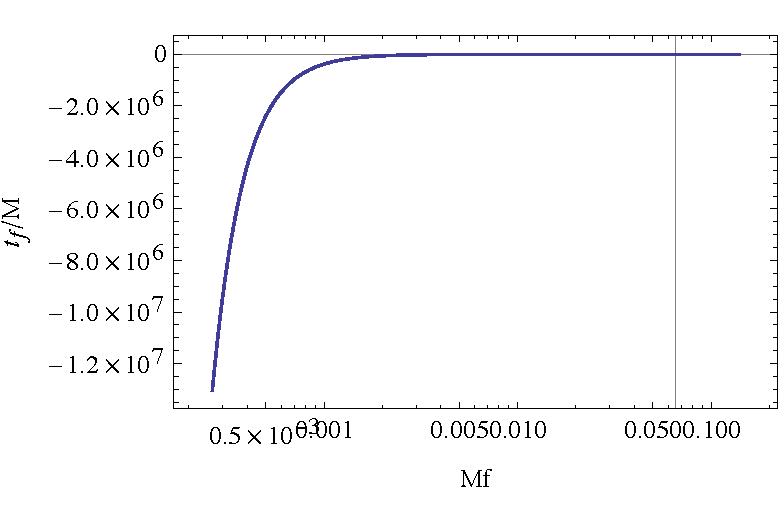
\includegraphics[width=.98\linewidth]{plots/tf.pdf}
  \caption{Time-to-frequency correspondence $t_{f}$, as defined directly from the phase of the Fourier-domain signal as in~\eqref{eq:deftf}, in geometric units. We show only the high-frequency part of the signal, corresponding to the merger region. The PhenomD waveforms have been aligned such that the time-domain amplitude (obtained by an IFFT \SM{[check acronym]}) peaks at $t=0$. The two aligned spins are equal, with components of $0.95$ ($++$, blue), $0$ ($00$, red), and $-0.95$ ($--$, yellow), for mass ratios $q=1$ (full line) and $q=8$ (dashed). The vertical lines shows the time-domain instantaneous frequency at the peak $\omega^{22}_{\rm peak}/(2\pi)$, again measured from an IFFT, and the fact that the curves $t_{f}$ do not pass exactly by the crossing with the $t=0$ horizontal line reflects the fact that the link between time-domain frequency and Fourier frequency $f$ is only approximate at merger. Note that $t_{f}$ increases to at most $\sim 30M$ after the peak, and is not monotonous. \SM{[add color to the vertical lines]} \SM{[add dots to highlights the crossings]}}
  \label{fig:tf}
\end{figure}

As a first step, we perform a formal leading-order expansion of the signal $\tilde{h}(f-f')$ around $f$. We use the amplitude/phase decomposition~\eqref{eq:defAPsi}, treat the Fourier-domain amplitude $A$ as a constant, expand the Fourier-domain phase $\Psi$ to the first order, and discard the $f'$ dependence in the first argument of $\tilde{G}(f-f', f')$, to obtain
\be
	\tilde{h}(f-f') \simeq A(f) \exp\left[ -i\left( \Psi(f) - f' \frac{\ud \Psi}{\ud f} \right) \right] \,,
\ee
Here and in the rest of the paper, such derivatives with respect to the frequency will always be evaluated at $f$.

Plugging this relation in~\eqref{eq:FDkernel}, we obtain
\begin{align}
	\tilde{s}(f) &\simeq \tilde{h}(f) \int \ud f' \, \exp\left[ i f' \frac{\ud \Psi}{\ud f} \right] \tilde{G}(f,f') \nn\\
	&= \tilde{h}(f) G\left( f, -\frac{1}{2\pi} \frac{\ud \Psi}{\ud f} \right) \,,
\end{align}
which motivates the introduction of an effective time, seen as a function of frequency,
\be\label{eq:deftf}
	\tf \equiv -\frac{1}{2\pi} \frac{\ud \Psi}{\ud f} \,.
\ee
It is worth noting that a shift in time of the time-domain signal will, by virtue of~\eqref{eq:shifttime}, be appropriately propagated to $t_{f}$. Because of the freedom of adding a linear term to $\Psi(f)$ by simply shifting the signal in time, no assumption can be made on the smallness of the first derivative of the phase, and this is really a leading order approximation.

The definition~\eqref{eq:deftf} is a generalization of the time-to-frequency correspondence at the heart of the SPA~\eqref{eq:deftfSPA}. Indeed, using~\eqref{eq:deftfSPA} one can verify that the derivative of the SPA phase $\Psi_{\rm SPA}$~\eqref{eq:PsiSPA} with respect to $f$ yields back $\tfSPA$, as
\be
	\tfSPA = -\frac{1}{2\pi} \frac{\ud \Psi_{\rm SPA}}{\ud f} \,.
\ee
However, our defintion~\eqref{eq:deftf} refers only to the Fourier-domain waveform. We do not need to relate the frequency $f$ to a time-domain frequency like the orbital frequency $\omega$, and the defintion is independent of the SPA being valid or not for the underlying signal $\tilde{h}$.

The main advantage of our time-of-frequency function~\eqref{eq:deftf} is that it extends naturally to the merger-ringdown part of the signals. Fig.~\ref{fig:tf} shows the behaviour of the time function $\tf$ around merger for six example waveforms, for mass ratios $q=1$ and $q=8$ and for aligned spin components $\chi=0.95,0.,-0.95$. In particular, one should note that $\tf$ is not monotonously increasing with frequency anymore when reaching in the high-frequency part of the waveform, corresponding to the ringdown. Although $t_{f}$ is always a well-defined function of $f$, this non-monotonicity would forbid an unambiguous definition of a reciprocal frequency-of-time function $f(t)$.

Using this notation, we have simply
\be\label{eq:transferlocal}
	\calT_{\rm local}(f) = G(f, \tf) = F(t_{f}) e^{-2i\pi f d(t_{f})}\,.
\ee
The interpretation of this approximation is straightforward: the signal is simply multiplied by the response function evaluated at the time $\tf$, the delay phase becoming the same linear phase contribution as one would have in~\eqref{eq:shifttime} with a time shift $d(t_{f})$ treated like a constant. The locality in frequency at $f$ for $\tilde{h}$ translates into a locality in time at $t_{f}$ for $F,d$.

%%%%%%%%%%%%%%%%%%%%%%%%%%%%%%%%%%%%

\subsection{Taylor expansion in the Fourier domain}
\label{subsec:TaylorFD}

We now extend our approach beyond the leading-order approximation. A Taylor-expansion of~\eqref{eq:FDkernel} in the variable $f'$ yields:
\begin{subequations}\label{eq:expandfprime}
\begin{align}
	\Psi(f-f') &= \Psi(f) + 2\pi f' \tf + \sum\limits_{p\geq 2}^{N} \frac{(-1)^{p}}{p!} {f'}^{p} \frac{\ud^{p} \Psi}{\ud f^{p}} \,, \label{eq:expandPsi}\\
	A(f-f') &= A(f) \sum\limits_{q\geq 0} \frac{(-1)^{q}}{q!} {f'}^{q} \frac{1}{A}\frac{\ud^{q} A}{\ud f^{q}} \,, \label{eq:expandA}\\
	\tilde{G}(f-f', f') &= \sum\limits_{r\geq 0} \frac{(-1)^{r}}{r!} {f'}^{r} \frac{\partial^{r} }{\partial f^{r}}  \tilde{G}(f,f') \label{eq:expandG} \,,
\end{align}
\end{subequations}
were we used the definition of $t_{f}$ introduced in~\eqref{eq:deftf}. In the following, we will only keep the first few terms in each of these expansions, but we keep these expressions in terms of formal series for now. Notice that we expand $\tilde{G}(f-f',f')$ in $f'$ only in its first argument, and that we can interchange the $f$-derivatives of $G$ with the Fourier transform operation.

Now, if we further expand the exponential of the phase to obtain a pure $f'$-expansion we can convert the resulting power series in $f'$ into a Taylor series with time derivatives, by applying the formal derivative rule
\allowdisplaybreaks
\be
	\int \ud f'\, {(-2i\pi f')}^{n} \frac{\partial^{m}}{\partial f^{m}} \tilde{G}(f,f') e^{-2i\pi f' \tf} = \frac{\partial^{m} }{\partial f^{m}} \frac{\partial^{n} }{\partial t^{n}} G (f,\tf) \,.
\ee
The result is a rather cumbersome expression with multiple sums, that we will not use directly. Instead, it will be more instructive to separate the different expansions in~\eqref{eq:expandfprime}. Only in Sec.~\ref{subsec:executivesummary} will we come back to combining our results together.

We first consider the effect of the higher-order corrections in~\eqref{eq:expandPsi}. We will find that the third and higher derivatives of the phase are always negligible for our purposes, and we will ignore them. Keeping only the first term of the series in~\eqref{eq:expandPsi}, corresponding to the second derivative of $\Psi$, and expanding the exponential of the phase, we obtain straightforwardly
\be\label{eq:resulttaylorPsi}
	\calT_{\rm phase}(f) = \sum\limits_{p\geq 0} \frac{1}{p!} \left( \frac{i}{8\pi^{2}}\frac{\ud^{2} \Psi}{\ud f^{2}} \right)^{p} \left( \frac{\partial^{2p} }{\partial t^{2p}} G \right)(f, \tf) \,.
\ee
This correction to the transfer function is of particular interest to us. It will be quantitatively dominant over the other ones in most contexts, and it will be shown in Sec.~\ref{subsec:resumquadphase} that it generalizes the previous approach of~\cite{KCY14}. This result shows that the transfer function is signal-dependent, not only through the time-to-frequency correspondence $t_{f}$ but also through the second derivative of the phase $\Psi$.

Similarly, the expansion of the Fourier-domain amplitude~\eqref{eq:expandA} gives
\be\label{eq:resulttaylorA}
	\calT_{\rm amp}(f) = \sum\limits_{p\geq 0} \frac{1}{(2i\pi)^{p}p!} \frac{1}{A} \frac{\ud^{p} A}{\ud f ^{p}}  \left( \frac{\partial^{p} }{\partial t^{p}} G \right)(f,\tf) \,,
\ee
while expanding only the frequency-dependence of $G$ as in~\eqref{eq:expandG} yields
\be\label{eq:resulttaylordelay}
	\calT_{\rm delay}(f) = \sum\limits_{p\geq 0} \frac{1}{(2i\pi)^{p}p!} \left( \frac{\partial^{p} }{\partial f^{p}} \frac{\partial^{p} }{\partial t^{p}} G \right)(f,\tf) \,,
\ee
which interestingly looks like a Taylor expansion of $G$, but this time with joint derivatives in frequency and time. This last expansion, taken separately from the other corrections, is signal-independent as it only depends on the function $G$ and not on $A$, $\Psi$.

As will be explained in Sec.~\ref{subsec:executivesummary}, we will also use these formal Taylor expansions to build error measures (constructed as the magnitude of the first term ignored in the series, see~\eqref{eq:deffom}) designed to estimate which of these three types of corrections are important to take into account.

%%%%%%%%%%%%%%%%%%%%%%%%%%%%%%%%%%%%

\subsection{Signal-dependent timescales}
\label{subsec:timescales}

\begin{figure}
  \centering
  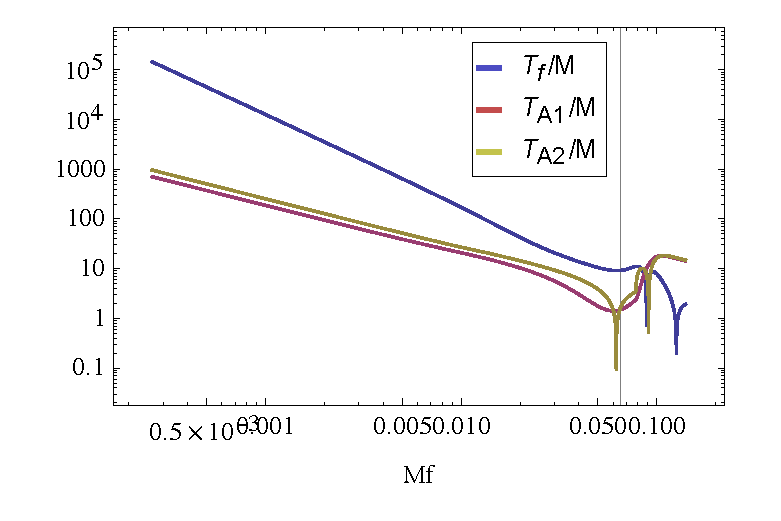
\includegraphics[width=.99\linewidth]{plots/TfTA.pdf}
  \caption{Fourier-domain amplitude and phase timescales, as defined in~\eqref{eq:defTf} and~\eqref{eq:defTA}, in geometric units for an equal-mass, non-spinning system. The hierarchy of these timescales is roughly the same for higher mass ratio and higher spin systems. The time-domain frequency at merger is represented by the vertical line. The derivatives from which these timescales are built encounter zero-crossings and change sign in the high-frequency range. \SM{[discuss discontinuity of third derivative]}\SM{[add vertical line for RD, make merger thick]}}
  \label{fig:TfTA}
\end{figure}

Considering~\eqref{eq:resulttaylorPsi} it is natural to define a new timescale, as a function of frequency, as
\be\label{eq:defTf}
	\Tf^{2} = \frac{1}{4\pi^{2}}\left| \frac{\ud^{2}\Psi}{\ud f^{2}} \right| \,.
\ee
The interpretation of this timescale for the inspiralling part of the signal, when the SPA applies, will be discussed below. We can use this notation to rewrite~\eqref{eq:resulttaylorPsi} as
\begin{align}\label{eq:resultdffPsiTf}
	 \calT_{\rm phase}(f) &= \sum\limits_{p\geq 0} \frac{(-i\epsilon)^{p}}{2^{p}p!} \Tf^{2p} \left( \frac{\partial^{2p} }{\partial t^{2p}} G \right)(f, \tf) \,,
\end{align}
where $\epsilon = -\mathrm{sgn}(\ud^{2}\Psi/\ud f^{2} )$ is $1$ in the inspiral.

We can obtain a straighforward physical interpretation of this timescale $\Tf$ by considering inspiral signals for which the SPA is valid. If we define
\be\label{eq:TfSPA}
	\Tf^{\rm SPA} \equiv \frac{1}{\sqrt{2\dot{\omega}(\tfSPA)}} \,,
\ee
we have, by taking two derivatives of~\eqref{eq:PsiSPA},
\be
	\left(\Tf^{\rm SPA} \right)^{2} = -\frac{1}{4\pi^{2}}  \frac{\ud^{2} \Psi_{\rm SPA}}{\ud f^{2}} \,,
\ee
where $\ud^{2}\Psi/\ud f^{2} < 0$ in the SPA with our sign conventions. The quantity $\Tf^{\rm SPA}$ is clearly a radiation-reaction timescale: the shorter this timescale, the faster the binary chirps to higher frequencies on its quasi-circular inspiral. Comparing with~\eqref{eq:defTf} above, we see that our generalized time scale $\Tf$ also reduces to $\Tf^{\rm SPA}$ when the SPA applies.

However, in the same way as our definition~\eqref{eq:deftf} for the time-of-frequency function $t_{f}$ generalizes the SPA definition~\eqref{eq:deftfSPA}, the definition~\eqref{eq:defTf} only refers to the phase of the Fourier-domain signal, does not require to introduce a time-domain frequency like $\omega$, and extends naturally to the merger-ringdown part of the signal. In this part of the signal, its physical interpretation as the timescale of radiation reaction is obscured, and the second derivative $\ud^{2}\Psi/\ud f^{2}$ can go through zero and change sign, as shown in Fig.~\ref{fig:TfTA}. We include an absolute value in the definition~\eqref{eq:defTf} to allow for this possibility, and keep track of the sign via $\epsilon$.

The expansion in amplitude corrections~\eqref{eq:resulttaylorA} also leads to the natural introduction of a set of other timescales related to the successive derivatives of the amplitude. In an analogous manner to the definition~\eqref{eq:defTf} of the timescale $\Tf$, we can define
\be\label{eq:defTA}
	\left( T_{Ap} \right)^{p} \equiv \frac{1}{(2 \pi)^{p}} \frac{1}{A(f)} \left| \frac{\ud^{p} A}{\ud f^{p}} \right| \,,
\ee
where we included an absolute value to accomodate the possible sign changes in the right-hand side. With this notation, \eqref{} becomes simply
\be\label{eq:resulttaylorA}
	\calT_{\rm amp}(f) = \sum\limits_{p\geq 0} \frac{1}{p!} (T_{Ap})^{p}  \left( \partial_{t}^{p} G \right) (f,\tf) \,,
\ee
Although the above is written for a generic $p\geq 0$, in practice only the first few of these timescales will be relevant. In this paper we will use only the first two, $T_{A1}$ and $T_{A2}$.

By contrast, the expansion~\eqref{eq:resulttaylordelay} is signal-independent and does not lead to the introduction of new timescales as the coupled time- and frequency derivatives are dimensionless. We will see however in Sec.~\ref{subsec:sizecorrLISA} that treating delays requires to take into account dimensionless factors of the type $2\pi f d$.

We can obtain useful estimates for these timescales from the Newtonian expressions~\eqref{eq:SPAN}. This gives for the Newtonian radiation-reaction and amplitude timescales:
\begin{subequations}\label{eq:timescalesN}
\begin{align}
	\Tf^{\rm N} &= \frac{1}{8} \sqrt{\frac{5}{3\nu}} \frac{G m}{c^{3}} v^{-11/2} \,, \label{eq:TfN}\\
	T_{A1}^{\rm N} &= \frac{7}{6} \frac{1}{2\pi f}\,, \quad T_{A2}^{\rm N} = \frac{\sqrt{91}}{6} \frac{1}{2\pi f} \,. \label{eq:TA1N-TA2N}
\end{align}
\end{subequations}
One can check explicitly that this expression for $\Tf$ agrees with~\eqref{eq:TfSPA}. With a simple power-law amplitude as in~\eqref{eq:ASPAN}, all higher-order amplitude timescales are also simply proportional to $1/f$ and differ only by their numerical factor.

We show in Fig.~\ref{fig:TfTA} the timescales $\Tf$, $T_{A1}$, $T_{A2}$ for an equal-mass and non-spinning system. In the inspiral, they follow the scalings~\eqref{eq:timescalesN} and $\Tf$ is much larger than the other two. For frequencies above the merger frequency, $\Tf$ can go through zero and the amplitude-related timescales become comparable or larger.

%%%%%%%%%%%%%%%%%%%%%%%%%%%%%%%%%%%%

\subsection{Quadratic term in the phase and relation to the SUA}
\label{subsec:resumquadphase}

If we restrict to the case of a pure modulation, $d=0$ and $G(f,t) = F(t)$, we can relate our result~\eqref{eq:resultdffPsiTf} to the approach of Ref.~\cite{KCY14}, where the authors extend the SPA in a formalism called the Shifted Uniform Asymptotic expansion (SUA) \SM{[look for other reference beyon KCY]}.
%The derivation includes an expansion of the modulation in Bessel functions, a study of the displacement of the stationary phase point induced by the precession, and a resummation of the result in the form of time derivatives.
The main intermediate result of~\cite{KCY14}, their equation~(34), reads exactly like~\eqref{eq:resultdffPsiTf} with $\epsilon=1$ and with the identifications $\tilde{H}_{corr}(f)\rightarrow \calT(f)$ for the transfer function, $T\rightarrow \Tf$ for the radiation-reaction timescale and $e^{-i\delta\phi} \rightarrow F$ for the modulation function (which is restricted in their framework to a phase, amplitudes being treated jointly with the amplitude of the signal). Thus, our treatment gives a straightforward rederivation of the result of~\cite{KCY14} which corresponds in our framework to the approximation~\eqref{eq:expandPsi}, where in the Fourier-domain convolution the phase of the signal is expanded to quadratic order and the amplitude is not expanded. The main difference is that the approach of~\cite{KCY14} still relies on the SPA being valid for the underlying signal.

The authors of~\cite{KCY14} then proposed a resummation scheme for~\eqref{eq:resultdffPsiTf}, using finite differences for the derivatives. Indeed, the result~\eqref{eq:resultdffPsiTf} looks like a symmetrized Taylor expansion, except for the factors $i^{p}$ and $1/p!$ instead of $1/(2p)!$. Truncating the sum at some finite order $N$, one can write (following~\cite{KCY14})
\be
	\calT_{\rm phase}(f) \simeq \sum\limits_{p = 0}^{N} \frac{(-i\epsilon\Tf^{2})^{p}}{2^{p}p!} \partial_{t}^{2p}F(\tf) \simeq \calF_{\Tf}^{N,\epsilon}[F] (\tf) \,,
\ee
with the operator $\calF_{T}^{N,\epsilon}$ defined as
\be
	\calF_{T}^{N,\epsilon}[F] (t) \equiv \frac{1}{2}\sum\limits_{k=0}^{N} a_{N,k}^{\epsilon} \left( F(t + kT) + F(t - k T) \right) \,,
\ee
provided that the complex coefficients $a_{N,k}^{\epsilon}$ are a solution of the $N+1$-dimensional linear system~\cite{KCY14}
\be\label{eq:stencilsystem}
	(-i\epsilon)^{p} (2p-1)!! = \sum\limits_{k=0}^{N} a_{N,k}^{\epsilon} k^{2p} \quad \text{for } p=0,\dots,N \,.
\ee
In~\cite{KCY14}, only the case $\epsilon=1$ was considered. The two solutions for the stencil coefficients in the two cases $\epsilon = \pm 1$ are simply related by a complex conjugation. Explicit expressions for the stencil coefficients $a_{N,k}^{\epsilon}$ are given in App.~\ref{app:stencil} for the first values of $N$.

An immediate advantage of this reformulation is its improved numerical stability. For the signal of precessing binaries, although one should expect an ideal scaling $\partial_{t}^{p} F \sim \Omega^{p} F$ with $\Omega$ the precession frequency, it can be extremely hard to control numerical derivatives of $F$ (which in any realistic model will be only provided as sampled at discrete times) well enough to enforce this scaling. Here, however, one simply evaluates the original smooth function $F$ at shifted times.

Note that the choice of the samples $\tf \pm k\Tf$ to approximate the successive derivatives of the expansion by finite differences, even if simple and natural, is by no means unique. Its structure leads to simple rational expressions for the stencil coefficients $a_{N,k}$, which will be given in~\ref{app:vandermonde} \SM{[refer to table]}. In principle, one could have made any ansatz of samples for the series expansion to be matched on. One cannot expect all choices to work equally well when applied to noisy data, and the problems of the numerical size of the coefficients and of the overall numerical stability of the scheme must be investigated numerically. We leave a more complete investigation of the asymptotics and numerical stability of this resummation approach for future work.

%%%%%%%%%%%%%%%%%%%%%%%%%%%%%%%%%%%%

\subsection{Relation to the Fresnel transform}
\label{subsec:fresneltransform}

We can give an alternative interpretation of~\eqref{eq:resultdffPsi} and of Sec.~\ref{subsec:resumquadphase} above by using an integral approach. For simplicity of notation, here we will again keep to the case of precessing binaries, with only a modulation $F$ and no delays, $d=0$. We will reintroduce the delays below in Sec.~\ref{subsec:delays}. To obtain~\eqref{eq:resultdffPsi}, we expanded fully the exponential as a Taylor series. If it is not expanded, however, we have
\be\label{eq:integralquadphase}
	\tilde{s}(f)	\simeq \tilde{h}(f) \int \ud t\, F(t) \int\ud f'\, e^{2i\pi f' (t-\tf)} \exp\left[ 2i\pi^{2} \epsilon{f'}^{2} \Tf^{2} \right] \,,
\ee
where we recall that $\epsilon = -\mathrm{sgn}(\ud ^{2} \Psi/\ud f^{2})$. The integral on $f'$ is a simple complex Gaussian integral, and results in a complex Gaussian integral over time where we recognize a Fresnel transform~\cite{} \SM{[C]} of the function $F$. We introduce for the Fresnel transform the notation
\be\label{eq:defFresnel}
	\calF_{\tau}[F](t_{0}) \equiv \frac{e^{i\frac{\pi}{4}}}{\sqrt{2\pi} \tau} \int \ud t \, \exp\left[ - \frac{i}{2} \left( \frac{t-t_{0}}{\tau} \right)^{2}\right] F(t) \,,
\ee
together with the additional notation
\be\label{eq:Fresnelsign}
	\calF^{\epsilon}_{\tau}[F](t_{0}) \equiv
\begin{cases}
	 \calF_{\tau}[F](t_{0}) &\text{ if } \epsilon=1 \\
	 \calF_{\tau}[F^{*}](t_{0})^{*} &\text{ if } \epsilon=-1
\end{cases}
\ee
to accomodate for the possible sign change represented by $\epsilon$. The integral~\eqref{eq:integralquadphase} then reads
\be\label{eq:resultFresnel}
	\tilde{s}(f) = \tilde{h}(f) \calF^{\epsilon}_{\Tf}[F](\tf) \,.
\ee

The Fresnel transform is an integral transform that shares some properties with the Fourier transform. It intervenes in particular in the theory of diffraction~\cite{} \SM{[C]}. Contrarily to the Fourier transform, however, it is localized in the sense that the part of the integral that is centered around $t_{0}$ contributes predominantly, due to the cancelling oscillations far from $t_{0}$. Note also that only the part of the function $F$ that is symmetric about $t_{0}$ contributes to the integral in~\eqref{eq:defFresnel}.

The parameter $\tau$ of the transform plays the role of a focusing parameter, determining how local the transform is. In the limit $\tau\rightarrow 0$, fast oscillations away from the central value $t_{0}$ will cancel out, leading to the integral taking the value $F(t_{0})$. For large values of $\tau$, however, the integral~\eqref{eq:defFresnel} has an extended support. Transposed in terms of the timescale $\Tf$, since we have seen that $\Tf$ can be interpreted as the radiation reaction timescale in the SPA regime, this means that a faster-chirping signal ($\Tf$ small) will have a Fresnel transform that is more focused, whereas a slower-chirping signal ($\Tf$ large) will have a Fresnel transform that is more extended. How much the Fresnel transform is focused in time is to be put in relation with how fast the function $F(t)$ in the integrand is varying. In the case of signals from precessing binaries, the precession timescale evolves as the system gets closer to merger, as will be discussed in details in~\ref{subsec:sizecorrPrec} below. In the case of the response of a LISA-like detectors, the modulation evolves with a timescale of one year, as will be detailed in Sec.\ref{subsec:sizecorrLISA}.

Although it is interesting to be able to relate our results to a known transformation used in signal processing, whether this opens avenues for more efficient computation methods remains to be investigated, for instance by performing a decomposition of the modulation $F$ in chirplets, which have analytically computable Fresnel transforms. Note that in the result~\eqref{eq:resultFresnel}, both the scale $\Tf$ and the central time $\tf$ are functions of the frequency $f$.

As a verification, upon performing a formal Taylor expansion in time of $F(t)$ around $\tf$ in the above integral and integrating term by term the result\footnote{Note that the intermediate integrals produced by such a Taylor expansion are formally divergent. One can regularize them for instance by introducing a small imaginary part in $\tau$ that is sent it to $0$ at the end of the computation.}, one readily recovers our previous result~\eqref{eq:resultdffPsiTf}. Now, the resummation of~\eqref{eq:resumquadphase} can be rephrased as a quadrature rule for computing the Fresnel integral~\eqref{eq:defFresnel}, according to
\be\label{eq:Fresnelstencil}
	\calF_{\tau}^{\epsilon} [F](t_{0}) \simeq \frac{1}{2} \sum\limits_{k=0}^{N} a_{N,k}^{\epsilon} \left( F(t_{0} + k\tau) + F(t_{0} - k\tau) \right)\,,
\ee
with $a_{N,k}^{1} = a_{N,k}$ and $a_{N,k}^{-1} = a_{N,k}^{*}$. Formally, if one allows for polynomial integrands in~\eqref{eq:defFresnel} (which can only be given sense by introducing a regularization), Eq.~\eqref{eq:Fresnelstencil} amounts to the building a quadrature rule for the particular choice of nodes $t_{0} \pm k \tau$, which is exact (with a regularization) if $F$ is a symmetric polynomial of degree $\leq 2N$. Note however that this quadrature rule does not fall into the class of Gaussian quadratures, which provide $N$-point rules that give an exact representation of the integral for polynomials of degree $2N-1$. Due to the complex character of the kernel in~\eqref{eq:defFresnel}, the induced inner product is not positive definite and some key properties are lost, such as the construction of the optimal Gaussian nodes from the zeros of the orthonormalized polynomials. For more details on quadrature rules when applied to integrals with oscillatory kernels, we refer to~\cite{} \SM{[C]}.

%%%%%%%%%%%%%%%%%%%%%%%%%%%%%%%%%%%%

\subsection{Treatment of the delays}
\label{subsec:delays}

In the case of a LISA-type detector response, the presence of the delay $d(t)$ is responsible for the frequency-dependence of the kernel $G$ introduced in~\eqref{eq:defg}. We will show below in Sec.~\ref{} \SM{[R]}that the higher-order correction in the delay can become non-negligible at high frequencies, as measured by the magnitude of the first correction in~\eqref{eq:taylordelay}. This is especially true for the orbital delay related to the motion of the whole detector constellation around the Sun, due to the large baseline for this delay.

Here we give an alternative treatment of the delays which is an alternative to the mere Taylor expansion of~\eqref{eq:taylordelay}. It is useful to look first at the case where one neglects the signal-related amplitude and phase corrections as given in~\eqref{eq:resultdfA} and~\eqref{eq:resultdffPsiTf}, but keeps the frequency-dependence in the convolution kernel in~\eqref{eq:defg}. The response then depends on the signal only by the time-to-frequency correspondence and reads
\begin{equation}
	\tilde{s}(f) = \tilde{h}(f) \int \ud t \, F(t) e^{-2i\pi f d(t)} \int \ud f' \, e^{2i\pi f' (t+d(t) - t_{f})} \,,
\end{equation}
where we recall that we defined $t_{f} \equiv -1/(2\pi)\ud \Psi/\ud f$. This motivates the introduction of the delayed time function $t_{d}:t \mapsto t+d(t)$, and of the reciprocal function $t_{d}^{-1}$, and of a modified time-to-frequency correspondence $\tfd = t_{d}^{-1}(\tf)$, defined implicitly by
\be
	\left. (t + d(t) - t_{f})\right|_{t=t_{f}^{d}} = 0 \,.
\ee
The above integral can then be formally computed as
\begin{align}\label{eq:delaycorrleading}
	\tilde{s}(f) &= \tilde{h}(f) \int \ud t \, F(t) e^{-2i\pi f d(t)} \delta(t + d(t) - t_{f}) \nn \\
	&= \tilde{h}(f) F(t_{f}^{d}) \frac{e^{-2i\pi f d(t_{f}^{d})}}{1+\dot{d}(t_{f}^{d})}
\end{align}

For the standard LISA configuration, we have for the orbital delays the scaling $d_{O}\sim R/c \sim 500s$, for the constellation delays the scaling $d_{c}\sim L/c \sim 8s$ (with $c=1$ and ignoring the dependence on angular factors). Since the motion of the constellation is periodic with a period of one year and $\Omega_{0} \simeq 2 \times 10^{-7}\mathrm{rad}.s^{-1}$, we have $\dot{d}_{O} \sim \Omega_{0} R/c \simeq 10^{-4}$ and $\dot{d}_{c} \sim \Omega_{0} L/c \simeq 1.7 \times 10^{-6}$. The smallness of the dimensionless quantity $\dot{d} \ll 1$ (and of its subsequent derivatives) will allow us to treat it perturbatively with a very good approximation, and shows also that the function $t_{d}$ is univalued and that there is no ambiguity in defining its reciprocal $t_{d}^{-1}$.

By treating $\dot{d}$ as a perturbation and keeping only first-order terms, we obtain for the delayed time reciprocal function
\begin{align}
	t_{d}^{-1}(t) &\simeq t-d(t) (1-\dot{d}(t)) \,,\nn\\
	d(t_{f}^{d}) &\simeq d(t_{f}) ( 1 - \dot{d}(t_{f})) \,.
\end{align}
Now, the most relevant correction in~\eqref{eq:delaycorrleading} comes from the phase factor at high frequencies, where the factors $2\pi f d_{O}$ and $2\pi f d_{c}$ give a magnification by a factor of, respectively, $3.10^{3}$ and $10^{2}$ at $1\Hz$. Ignoring the other corrections, we thus arrive at the approximate form for the transfer function
\be
	\calT(f) \simeq F(t_{f})\exp\left[ -2i\pi f d(t_{f}) (1-\dot{d}(t_{f})) \right] \,.
\ee
Notice that this leading-order correction in the treatment of the delays affects purely the phase of the signal.

Next, we consider the case where the quadratic phase correction is kept as well, as in Sec.~\ref{subsec:fresneltransform}. Keeping as before only the first-order terms in $\dot{d}$ (and neglecting its higher derivatives), we can write
\begin{widetext}
\begin{align}
	\tilde{s}(f) &\simeq \tilde{h}(f) \int \ud t \, F(t) e^{-2i\pi f d(t)} \int \ud f' \, \exp\left[ 2i\pi \epsilon \Tf^{2} f'^{2} + 2i\pi f' (t+d(t) - \tf) \right] \nn\\
	&\simeq \tilde{h}(f) \frac{e^{i\epsilon\frac{\pi}{4}}}{\sqrt{2\pi}\Tf} \int \ud \tau \, \frac{F(\tau - d(\tau))}{1+\dot{d}(\tau)} e^{-2i\pi f d(\tau)(1-\dot{d}(\tau))}\exp\left[ -\frac{i\epsilon}{2} \frac{(\tau - \tf)^{2}}{\Tf^{2}} \right] \,,
\end{align}
\end{widetext}
where we used a change of variable $\tau = t_{d}(t)$. We see that the result can again be expressed as a Fresnel transform. When considering amplitude corrections as well, as in~\eqref{}, additional powers of $f'$ can be translated as time derivatives with respect to the variable $\tau$ after performing the change of variables. This produces our most general result given in Eq.~\eqref{eq:transferfinal} below.

\subsection{Executive summary of the formalism}\label{subsec:executivesummary}

In this Section, we gather our previous results for the convenience of the reader. For a modulation $F$ and delay $d$, so that $s(t) = F(t) h(t+d(t))$, we defined the associated function $G(f,t) = F(t) e^{-2i\pi f d(t)}$ and we obtained the transfer function $\calT (f) = \tilde{s}(f)/\tilde{h}(f)$:
\begin{widetext}
\be\label{eq:transferfinal}
	\calT(f) = \sum\limits_{k \geq 0} \frac{(-i)^{k}}{k!} (T_{Ak})^{k} \calF^{\epsilon}_{\Tf} \left[ \frac{\ud^{k}}{\ud \tau^{k}} \left( \frac{F(\tau - d(\tau))}{1+\dot{d}(\tau)} e^{-2i\pi f d(\tau)(1-\dot{d}(\tau))} \right) \right] (\tf) \,.
\ee
\end{widetext}
In each term of this series, the Fresnel transform $\calF^{\epsilon}_{\Tf}$ can in turn be approximated by using the stencil formula~\eqref{eq:Fresnelstencil}. The timescales $\Tf$ and $T_{Ak}$ were defined in~\eqref{eq:defTf} and~\eqref{eq:defTA}, and the generalized time-to-frequency function $t_{f}$ was given in~\eqref{eq:deftf}. The delays $d$ are present only in the LISA context, while in the context of precessing binaries we only have to consider the modulation function $F$. In practice, only the first few of the terms in this last remaining series expansion are relevant. We will investigate several orders of approximation, combining corrections from the phase, amplitude and delays, and explore which ones are relevant for a given level of accuracy. We will use symbols of the form $\{N,A,d\}$ to indicate the order of the stencil in~\eqref{eq:Fresnelstencil}, the maximal order of the amplitude correction included, and the inclusion or not of the delay correction.

In the LISA context, due to the smallness of the corrections we will only go up to \SM{[k=2 for prec]} $k=1$ in~\eqref{eq:transferfinal}, and in computing the remaining time derivatives in~\eqref{eq:transferfinal} we will neglect the second and higher derivatives. We will also use $F(\tau - d(\tau)) \simeq (F - d \dot{F})(\tau)$. This gives concretely:
\begin{widetext}
\begin{subequations}
\begin{align}
	\{N,A:0,d:0\}&: \; \calT(f) = \calF^{\epsilon}_{\Tf} \left[ F e^{-2i\pi f d} \right] (t_{f}) \,, \\
	\{N,A:1,d:0\}&: \; \calT(f) = \calF^{\epsilon}_{\Tf} \left[ \left(F - i T_{A1} \left( \dot{F} - 2i\pi f \dot{d}\right) \right) e^{-2i\pi f d} \right] (t_{f}) \,, \\
	\{N,A:0,d:1\}&: \; \calT(f) = \calF^{\epsilon}_{\Tf} \left[ \frac{F - d\dot{F}}{1+\dot{d}} e^{-2i\pi f d (1-\dot{d})} \right] (t_{f})\,, \\
	\{N,A:1,d:1\}&: \; \calT(f) = \calF^{\epsilon}_{\Tf} \left[ \frac{1}{1+\dot{d}}\left(  F - d\dot{F} - i T_{A1} \left( \dot{F} - 2i\pi f \dot{d} \right) \right) e^{-2i\pi f d (1 - \dot{d})} \right] (t_{f})\,.
\end{align}
\end{subequations}
\end{widetext}

In the context of precessing binaries, the delays are absent and we will go up to $k=2$ in~\eqref{eq:transferfinal}. The orders of approximation will be:
\begin{subequations}
\begin{align}
	\{N,A:0\}&: \; \calT(f) = \calF^{\epsilon}_{\Tf} \left[ F \right] (t_{f}) \,, \\
	\{N,A:1\}&: \; \calT(f) = \calF^{\epsilon}_{\Tf} \left[ \left(F - i T_{A1} \dot{F} \right) \right] (t_{f}) \,, \\
	\{N,A:2\}&: \; \calT(f) = \calF^{\epsilon}_{\Tf} \left[ \left(F - i T_{A1} \dot{F} - \frac{1}{2} (T_{A2})^{2} \ddot{F} \right) \right] (t_{f}) \,.
\end{align}
\end{subequations}

In the following, it will be convenient to introduce error estimates built from the Taylor-like series~\eqref{eq:resulttaylorPsi},~\eqref{eq:resulttaylorA} and~\eqref{eq:resulttaylordelay}. We simply define  this error estimates at a certain level of approximation as the magnitude of the first term ignored in the original Taylor series. Thus we define \SM{[check if the 1/2! was taken into account]}
\SM{[interpretation of $\epsilon$'s as ratios of timescales - next subsec]}

\SM{[add magnitude of the derivatives of G, like $\Omega^{n}$ with possible factors of $2\pi f d$]}

\SM{[add loose convergence argument with scaling $\partial^{n}_{t} \sim \Omega^{n} $]}

\SM{[stress that these are errors in the relative sense - so less important in RD than it seems]}
\begin{subequations}\label{eq:deffom}
\begin{align}
	\epsilon_{\Psi 2} &\equiv \frac{1}{2} \Tf^{2} \left| \frac{1}{G}\partial_{tt}G \right| \,, \\
	\epsilon_{A 1} &\equiv T_{A1} \left| \frac{1}{G} \partial_{t} G \right| \,, \\
	\epsilon_{A 2} &\equiv \frac{1}{2} T_{A2}^{2} \left| \frac{1}{G} \partial_{tt}G \right| \,, \\
	\epsilon_{d} &\equiv \frac{1}{2\pi} \left| \frac{1}{G} \partial_{tf} G \right| \,,
\end{align}
\end{subequations}
where the function $G$ and its derivatives are evaluated at $(f, t_{f})$. Reaching $\epsilon \simeq 1$ will indicate a breakdown of the perturbative approach. As we will detail below, in the presence of delays these derivatives do not obey the simple scaling $\partial_{t}^{n} \rightarrow \Omega_{0}^{n}$, with $\Omega_{0}$ the characteristic frequency for the time variablility in the modulation and delay. This is due to the presence of additional dimensionless delay terms of the form $2\pi f d$, which can be larger than 1.

We will also \SM{[]}

%%%%%%%%%%%%%%%%%%%%%%%%%%%%%%%%%%%%
%%%%%%%%%%%%%%%%%%%%%%%%%%%%%%%%%%%%

\section{Application to the response of LISA-type detectors}
\label{sec:LISA}

%%%%%%%%%%%%%%%%%%%%%%%%%%%%%%%%%%%%

\subsection{The response model}
\label{subsec:modelLISA}

In this Section, we expand Sec.~\ref{subsec:} \SM{[R]} and detail more the model that we use for the response of a LISA-like detector, together with the assumptions used and their limitations.

As argued in~\cite{Krolak+04} \SM{[expand a bit; not the only place where this approximation is used]}, since we focus on the gravitational-wave contribution to the basic observable, we can use a simplified model for the response, ignoring corrections that are crucial from the point of view of noise cancellations. Our aim is indeed to assess the accuracy of a direct Fourier-domain treatment of the response, thus focusing on the separation of timescales in the problem, keeping in mind that corrections can be added later without affecting the conclusions of the present analysis.

The frequency-shift response for a single link~\eqref{eq:yslr} was derived in Ref.~\cite{EW75} (see also~\cite{RCP04, Finn08, Cornish09} for more modern derivations). Several assumptions enter the result as written in~\eqref{eq:yslr}: (i) effects of the order $v/c$ are neglected, including for instance the special relativistic Doppler effect created by the relative speeds of the spacecrafts on their orbits (ii) the propagation is assumed to take place in a flat spacetime, perturbed only by the gravitational wave; thus the gravitational redshift as well as the deflection of light created by the gravitational potential of the Sun is ignored (iii) all geometric factors are evaluated at a single time, whereas one should consider the beam as propagating from the position of the first spacecraft at the time of emission to the position of the second scapecraft at the time of reception, leading to a pointing-ahead effect.

Additionally, we limit ourselves to a rigid model for the detector, namely we assume that the constellation remains in an equilateral configuration with fixed armlengths $L=2.5\times 10^{6}\mathrm{km}$, as proposed in~\cite{LISA17}. This simplified orbits neglect (iv) the effect of excentricity of the individual Keplerian orbits, which introduces corrections at the level $e^{2}$ (v) the effect of gravitational perturbations coming from other celestial bodies, such as the Earth, the quadrupole of the Sun, and the other planets. 

Note that although we can neglect all the effects (i)-(v) for our present study, keeping track of these corrections is crucial for the purpose of laser noise cancellations, and led to the development of new generations of TDI observables~\cite{} \SM{[C]}.

Since the orbital delay due to the orbit around the Sun is common to all $y_{slr}$ observables, we will decompose the one-arm instrument response~\eqref{} \SM{[R]} in two steps. The first step consists simply in applying the varying time delay to bring the signal from the SSB to the center of the LISA triangular constellation. For $h^{\rm TT}$ the transverse-traceless gravitational waveform in matrix form, we write this orbital time delay as
\be\label{eq:defresponseO}
	h_{O}^{\rm TT} (t) = h^{\rm TT}(t-\hatk\cdot p_{O}) \,.
\ee
The second step consists in the remaining, constellation-centered response, which we write as
\begin{align}\label{eq:defresponsec}
	y_{slr} &= \frac{1}{2} \frac{1}{1 - \hatk\cdot n_{l}} \nn\\
	& \cdot n_{l}\cdot \left[ h_{O}^{\rm TT}(t - L - \hatk\cdot p^{L}_{s}) - h_{O}^{\rm TT}(t - \hatk\cdot p^{L}_{r}) \right] \cdot n_{l}\,,
\end{align}
where we introduced the positions of the spacecrafts relative to the center of the constellation, $p^{L}_{A} \equiv p_{A} - p_{O}$.

We will decompose the full signal in the contributions of the individual spin-weighted spherical modes $h_{\ell m}$, whose Fourier transforms are assumed to have a smooth amplitude and phase. First, we define the matrices $P_{+},P_{\times}$ such that, in the sense of matrices,
\be
	h^{\rm TT} = h_{+}P_{+} + h_{\times}P_{\times} \,.
\ee
Assuming that the approximation~\eqref{eq:zeronegativef} applies, we focus only on positive frequencies and consider a mode contribution $h$ following~\eqref{eq:notationhsignm}. We can define a complex matrix $P$ incorporating the spin-weighted spherical harmonic constant factor as
\be
	P_{\ell m} = 
	\begin{cases} 
	\frac{1}{2} {}_{-2}Y_{\ell m} \left( P_{+} + i P_{\times} \right) \text{ for } m>0\,,\\
	\frac{1}{2} {}_{-2}Y_{\ell m}^{*} \left( P_{+} - i P_{\times} \right) \text{ for } m<0\,.
	\end{cases}
\ee

We now turn to the transposition of~\eqref{eq:defresponseO} and~\eqref{eq:dfresponsec} to the Fourier-domain. For the leading-order response~\eqref{eq:deflocal}, in what we call the local approximation, applying a pure delay as in~\eqref{eq:defresponseO} translates into Fourier-domain transfer function that is a pure phase factor, proportional to the frequency but also $t_{f}$-dependent: \SM{[check sign]}
\be\label{eq:transferOlocal}
	\calT_{O}^{\rm local}(f) = e^{-2i\pi f d_{O}(t_{f})}\,,
\ee
with $d_{O} = -\hatk \cdot p_{O}$ the orbital delay. When using the leading-order response~\eqref{eq:transferlocal} for the constellation response, the delays take similarly the form of pure phase factors. When also using the rigid approximation for the constellation, where the armlengths are fixed, a particular simplification occurs when combining these individual delays. The Fourier-domain transfer function then reads
\begin{align}\label{eq:transferclocal}
	\calT_{slr}^{\rm local} &= \frac{i \pi f L}{2} \sinc \left[ \pi f L\left(1-\hatk\cdot n_{l} \right) \right] \nn\\
	& \qquad \cdot \exp\left[ i \pi f \left( L + \hatk\cdot \left( p_{1}^{L} + p_{2}^{L} \right) \right) \right]  n_{l} \cdot P_{\ell m} \cdot n_{l} \,,
\end{align}
where all vectors $n_{l}$ and $p_{A}^{L}$ are to be evaluated at time $t_{f}$. We used the rigid-arms approximation relation $p^{L}_{r} - p^{L}_{s} =  L n_{l}$. The result~\eqref{eq:transferclocal} is familiar, as it was derived in the past taking the point of view of monochromatic signals (see e.g.~\cite{}).

In the case $m<0$, the formalism can be applied in the same way, except that notation is complicated by the fact that the mode $\tilde{h}_{\ell m}$ has to be evaluated at $-f$. In the following, we will limit ourselves to the case $m>0$ for simplicity of presentation. \SM{[really necessary ?]}

Note that, if the corrections~\eqref{} are included for the constellation delays, this transfer function will not have this simple form anymore, as $\dot{d}$ will have a different velocity-dependent expression for the sending and receiving spacecrafts.

It is natural to define two transfer frequencies for the two relevant length scales for the delays, defined such that a wavelength fits within this length scale. Geometrical projection factors aside, these scales are the radius of the orbit around the Sun $R=1\text{au}=1.5\times 10^{8} \text{km}$ and the detector armlength $L=2.5\times 10^{6}\text{km}$ (in the configuration proposed in~\cite{LISA17}). This gives
\begin{subequations}\label{eq:transferfrequencies}
\begin{align}
	f_{R} &= 3.2\times10^{-4}\text{Hz} \,\\
	f_{L} &= 1.9\times 10^{-2}\text{Hz} \,.
\end{align}
\end{subequations}
These transfer frequencies will indicate where in the LISA band a dimensionless delay term of the form $2\pi f d$ becomes larger than unity. \SM{[check if this appears elsewhere]}

\SM{[comment on the added structure in the high-f response - say a word of f-factor corresponding to discrete derivatives - define low-f response that others have been using - reference to folks also looking at that (marginal) for ET? ]}

%%%%%%%%%%%%%%%%%%%%%%%%%%%%%%%%%%%%

\subsection{Estimates for the magnitude of higher-order corrections}
\label{subsec:sizecorrLISA}

\SM{[add order-of-magnitude estimate for ET]}

\SM{[check if there is something to be done with recent paper on ET modulations]}

\SM{[add order-of-magnitude estimate for EMRIS]}

\SM{[possibly add order-of-magnitude estimate for geocentric-LISA ?]}

\SM{[justify somewhere smallness of cubic-in-phase term]}

\SM{[crude estimate of the target accuracy level: 1/SNR ?]}

\SM{[distinguish orbital from constellation at the level of orders of magnitude estimates: factor 2pif*d when taking derivatives of the transfer function for the pure delay]}

\SM{[change notations from O to 0 for orbital response, and check we use notations $\Omega_{0}$, $f_{0}$]}

Due to the smallness of the annual frequency $\Omega_{0}/2\pi \simeq 3.1\times10^{-8}\mathrm{Hz}$ compared to the timescales relevant for the signal over the LISA frequency band, one can expect that the higher-order corrections described in Section~\ref{sec:formalism} are small. In this Section we try to quantify to which extent, and give simple estimates of their magnitude.

Using the Newtonian-order expressions~\eqref{eq:timescalesN} for the signal-dependent timescales $\Tf$ and $T_{A1}$, we can obtain a useful order-of-magnitude estimate for the error measures $\epsilon$ introduced in~\eqref{eq:deffom}. Higher-order amplitude terms beyond the first one in~\eqref{eq:resulttaylorA} will turn out to be completely negligible in the LISA case and we will ignore them in the following. We will present these estimates separately for the orbital response~\eqref{eq:transferOlocal} and the constellation~\eqref{eq:transferclocal}, as the different baseline of the delays ($R$ or $L$) as well as the presence of a time-varying prefactor $F(t)$ both affect the result. As we will see, when estimating the magnitude of the relevant derivatives of $G$ we have to take into account delay factors of the type $2\pi f d$.

We start with the orbital response, which takes the form of a pure delay $G_{0}(f, t) = e^{-2 i \pi f d_{O}(t)}$, and obtain
\begin{subequations}
\begin{align}
	\frac{1}{G_{0}} \partial_{t} G_{0} &= -2i\pi f \dot{d}_{O}\,,\\
	\frac{1}{G_{0}} \partial_{tt} G_{0} &= -2i\pi f \ddot{d}_{O} - 4\pi^{2} f^{2} \dot{d}_{O}^{2} \,,\\
	\frac{1}{G_{0}} \partial_{tf} G_{0} &= -2 i \pi \dot{d}_{O} - 4\pi^{2} f d_{O} \dot{d}_{O} \,,
\end{align}
\end{subequations}

For the constellation response \SM{[say here that even the one-arm response is actually the difference between two G's, so the error measure is not quite rightly used -- origin of the f factor in front]}, since we wish to write errors in relative sense starting from the single-arm response~\eqref{eq:transferclocal} which is already analogous to a discrete time derivative of the signal, we keep explicit the overall factor $f$ reflecting this derivative. \SM{[investigate later how this applies to the discrete time derivatives that define the TDI - here we are allowed to ignore this because they are with a fixed L-delay]} We will write symbolically $G_{c}(f,t) \sim f F(t) e^{-2i \pi f d_{c}(t)}$, where $d_{c}$ represents the delay term and $F(t)$ represents the rest of the geometric factors in~\eqref{eq:transferclocal} where we ignore the $f$-dependence. This gives in this case
\begin{subequations}
\begin{align}
	\frac{1}{G_{c}} \partial_{t} G_{c} &\sim -2i\pi f \dot{d}_{c} + \frac{\dot{F}}{F}\,,\\
	\frac{1}{G_{c}} \partial_{tt} G_{c} &\sim -2i\pi f \ddot{d}_{c} - 4\pi^{2} f^{2} \dot{d}_{c}^{2} - 2i\pi f \dot{d}_{c} \frac{\dot{F}}{F} - \frac{\dot{F}^{2}}{F^{2}} + \frac{\ddot{F}}{F} \,,\\
	\frac{1}{G_{c}} \partial_{tf} G_{c} &\sim -4 i \pi \dot{d}_{c} - 2i\pi d_{c} \frac{\dot{F}}{F} - 4\pi^{2} f d_{c} \dot{d}_{c} + \frac{1}{f}\frac{\dot{F}}{F}\,.
\end{align}
\end{subequations}

In order to obtain simple scalings for the error estimates, we will make the replacements $\partial_{t}^{n} d \sim \Omega_{0}^{n} d$ as well as $\partial_{t}^{n} F \sim \Omega_{0}^{n} F$. These scalings are only approximate and the various possible orientation angles can lead to significant variations. We will assume $d_{0} \sim R_{\rm eff} $ (recalling that we set $c=1$ \SM{[check if that is consistently done throughout]}) with an effective orbit radius $R_{\rm eff} \equiv 2R/\pi$ representing an average of the geometric projection factor of the gravitational wave propagation vector on the plane of the orbit. For the constellation delays, we simply take $d_{c} \sim L$ as there projection effects can lead to variations in both ways. We build estimates for the magnitude of these derivatives as follows:
\begin{subequations}\label{eq:estimatederivorb}
\begin{align}
	\left| \frac{1}{G_{0}} \partial_{t} G_{0} \right| &\sim 2 \pi f \Omega_{0} R_{\rm eff}\,,\\
	\left| \frac{1}{G_{0}} \partial_{tt} G_{0} \right| &\sim \text{max} \left[ 2 \pi f \Omega_{0}^{2} R_{\rm eff} , 4\pi^{2} f^{2} \Omega_{0}^{2} R_{\rm eff}^{2}\right] \,,\\
	\left| \frac{1}{G_{0}} \partial_{tf} G_{0} \right| &\sim \text{max} \left[ 2 \pi  \Omega_{0} R_{\rm eff}, 4 \pi^{2} f \Omega_{0} R_{\rm eff}^{2} \right] \,,
\end{align}
\end{subequations}
for the orbital response and
\begin{subequations}\label{eq:estimatederivconst}
\begin{align}
	\left| \frac{1}{G_{c}} \partial_{t} G_{c} \right| &\sim \text{max} \left[ \Omega_{0}, 2 \pi f \Omega_{0} L \right] \,,\\
	\left| \frac{1}{G_{c}} \partial_{tt} G_{c} \right| &\sim \text{max} \left[ \Omega_{0}^{2}, 4 \pi f \Omega_{0}^{2} L, 4\pi^{2} f^{2} \Omega_{0}^{2} L^{2} \right] \,,\\
	\left| \frac{1}{G_{c}} \partial_{tf} G_{c} \right| &\sim \text{max} \left[ \Omega_{0}/f, 6 \pi \Omega_{0} L, 4\pi^{2} f \Omega_{0}^{2} L^{2} \right] \,,
\end{align}
\end{subequations}
for the constellation response. In the presence of different terms, we simply take the maximum of their norms. An important point in the above is the presence of delay factors in the forms of powers of $2\pi f d$. Thus, the magnitude of the corrections cannot be evaluated with the simple replacement $\partial_{t}^{n} \rightarrow \Omega_{0}^{n}$, and the frequency dependency of the error measures will depend on the frequency being above or below the transfer frequencies $f_{R}$ and $f_{L}$ defined in~\eqref{eq:transferfrequencies}.

The error measure $\epsilon_{d}$ does not depend on signal-dependent timescales and can be directly read off the estimates above, with $\epsilon_{d} = \partial_{tf}G/(2\pi G)$. For the error measures $\epsilon_{\Psi}$ and $\epsilon_{A1}$, we can combine the above with the Newtonian timescales given in~\eqref{eq:timescalesN} for the inspiral phase of the signal. An important distinction needs to be made there, as the radiation reaction timescale $\Tf$ grows rapidly towards lower frequencies as $f^{-11/6}$. If one considers systems that are arbitrarily far from merging, $\Tf$ can be made arbitrarily large, leading the error measure $\epsilon_{\Psi}$ to take values arbitrarily larger than 1 where the perturbative treatment we adopted breaks down. This limit would describe systems observed in their deep inspiral and very slowly chirping, such as the population of galactic binaries that form one of the science targets of the LISA mission~\cite{LISA17}. Such signals would be very compact in Fourier domain, and are not covered by our formalism that assumes an extended Fourier spectrum. We will present in App.~\ref{} \SM{[R]} another version of our formalism based on discrete Fourier coefficients, that could apply better to this case \SM{[check: do we put this appendix or not ?]}. On the contrary, if one considers only systems that will merge during or shortly after the observation span of the mission, the starting frequency of the observations will be set by this limited lifetime of the source before merging and we can then bound $\epsilon_{\Psi}$ to be smaller than 1.

In the following we will consider only these merging binaries, which include the supermassive black hole mergers that we expect to detect~\cite{LISA17}. The population of stellar-origin binary black holes, proposed in~\cite{Sesana16}, will have both sources rather far from merger and sources that will merge within a few years after the mission finishes. We will take a reference starting frequency corresponding to a time from merger $\Delta t = 10\text{yrs}$. Since the corrections turn out to be most important at the beginning of the signal, we will evaluate the timescales at this starting frequency. From the Newtonian relation~\eqref{eq:omegaphiN}, we have (using $\nu_{0} = 1/4$ for the equal-mass value): \SM{[check]}
\be
	f_{\rm start} = 2.9\times 10^{-5} \text{Hz} \left( \frac{\nu}{\nu_{0}} \right)^{-3/8} \left( \frac{m}{10^{6}M_{\odot}} \right)^{-5/8} \left( \frac{\Delta t}{10 \text{yr}} \right)^{-3/8} \,,
\ee
which gives in turn for the timescales
\begin{subequations}
\begin{align}
	\Tf = 6.8\times10^{-2}\text{yr} \left( \frac{\nu}{\nu_{0}} \right)^{3/16} \left( \frac{m}{10^{6}M_{\odot}} \right)^{5/16} \left( \frac{\Delta t}{10 \text{yr}} \right)^{11/16} \,\\
	T_{A1} = 2.0\times10^{-4}\text{yr} \left( \frac{\nu}{\nu_{0}} \right)^{3/8} \left( \frac{m}{10^{6}M_{\odot}} \right)^{5/8} \left( \frac{\Delta t}{10 \text{yr}} \right)^{3/8} \,.
\end{align}
\end{subequations}
\SM{[change notation for total mass everywhere to $M$]} When inserting these expressions in~\eqref{eq:deffom}, in~\eqref{eq:estimatederivorb} and~\eqref{eq:estimatederivconst} we must also use $f_{\rm start}$ for the possible extra factors of $f$ or $f^{2}$ coming from the delay terms, which can lead to different overall scalings with mass ratio and total mass depending on where the signal starts in the band.

We summarize the results for the error estimates in Fig.~\ref{fig:fomLISA}. We show the magnitude of the error estimates $\epsilon_{\Psi}$, $\epsilon_{A1}$, $\epsilon_{d}$ both for the orbital delay and the constellation response, for an equal-mass system with total masses of $m=10^{7} \Msol$, $10^{4} \Msol$ and $10^{2} \Msol$ and a starting frequency corresponding to $\Delta t =10 \text{yr}$ of observation. Since individual signals can show significant variation depending on the angular parameters, we show an average of $\ln \epsilon$ over the sky position, inclination and polarization, together with $\pm \sigma$ standard deviation, and overlay the estimates resulting from~\eqref{eq:estimatederivorb},~\eqref{eq:estimatederivconst} and~\eqref{eq:timescalesN}. Here and in the following, for completeness we show results on the frequency band from $10^{-5}\text{Hz}$ to $1Hz$, while the signals are expected to have little signal-to-noise ratio outside of the band from $10^{-4}\text{Hz}$ to $10^{-1}Hz$, which is sometimes taken as a reference~\cite{LISA17}.

For $\epsilon_{\Psi}$, we find as expected a steep rise towards lower frequencies, which shows that considering only merging binaries with a limited time remaining before merger is crucial here. Due to the different occurences of delay factors, we find a different behaviour between the orbital response, where the initial value of $\epsilon_{\Psi}$ grows towards lower masses, and the constellation response, where $\epsilon_{\Psi}$ grows towards higher masses. In both cases, the error measure remains below $\epsilon_{\Psi} \sim 0.1$, where the corrections can be sizeable but well manageable by the perturbative formalism (as we will show in the next Section). Not represented in the figure is the behaviour with mass ratio, which also differs: for a total mass of $10^{2} \Msol$, the extra factors of $f_{\rm start}$ due to the delay factors lead to an increase towards larger mass ratios, while for a total mass of $10^{7} \Msol$ we have a decrease towards larger mass ratios.

For $\epsilon_{A1}$, we find that the structure in the waveform close to merger does have a visible but limited impact on the error measure. For the orbital response, the error measure remains small for all masses. For the constellation response, we find that $\epsilon_{A1}$ can grow up to $\sim 0.01$ at the lower end of the frequency band for high masses. Since the timescale $T_{A1}^{\rm N}$ has a simple dependence $\propto 1/f$, these statements should hold for all mass ratios at least during the inspiral.

The $\epsilon_{d}$ is signal-independent, and follows a quite different behaviour for the orbital and constellation responses. For the orbital response, $\epsilon_{d_{0}}$ grows for higher frequencies, reaching the $\sim 0.1$ at around $1\text{Hz}$. For the constellation response, $\epsilon_{d_{c}}$ is mainly important at lower frequencies, reaching $\sim 0.01$ at around $10^{-5}\text{Hz}$.

Overall, we find that for merging binaries the perturbative approach presented in Sec.~\ref{} \SM{[]} will apply, with the most relevant higher-order corrections being expected to be the phase corrections close to the starting frequency of the signal and the delay correction at high frequencies for the orbital response.

\begin{figure*}
  \centering
  \includegraphics[width=.32\linewidth]{plots/lisafom_Psiorb.pdf}
  \includegraphics[width=.32\linewidth]{plots/lisafom_A1orb.pdf}
  \includegraphics[width=.32\linewidth]{plots/lisafom_dorb.pdf}
  %
  \includegraphics[width=.32\linewidth]{plots/lisafom_Psiconst.pdf}
  \includegraphics[width=.32\linewidth]{plots/lisafom_A1const.pdf}
  \includegraphics[width=.32\linewidth]{plots/lisafom_dconst.pdf}
  \caption{Error estimates of the approximation as defined in~\eqref{eq:deffom}, for an equal-mass, non-spinning system and for total masses of $10^{7} \Msol$, $10^{4} \Msol$ and $10^{2} \Msol$. The top row corresponds to the orbital delay part of the response~\eqref{eq:dfresponseO}, and the lower row shows the LISA-centered constellation response~\eqref{eq:dfresponsec}. The error estimates~\eqref{} \SM{[R]} are shown for the phase, amplitude and delay terms from left to right. The central line and interval are the mean and $1\sigma$ standard deviation of the logarithm of $\epsilon$ over 400 random values for the position in the sky, inclination and polarization. The starting frequency is set by an observation time of $\Delta t = 10 \text{yrs}$ before merger. \SM{[change middle mass to $3\times 10^{4}$ ? - clarify mismatch between these $\epsilon$ and the actual size of corrections]}}
  \label{fig:fomLISA}
\end{figure*}

%%%%%%%%%%%%%%%%%%%%%%%%%%%%%%%%%%%%

\subsection{Error control for the Fourier-domain response}
\label{subsec:errorsLISA}

\SM{[We have to say why we take a non-spinning, equal-mass system - say why the method should also work for precessing signals]}

\SM{[Write explicitly what the orders A1, d1 mean]}

\SM{[argument why we do not compute mismatches]}

\SM{[stress that binaries very far from merger could have arbitrarily large Psi2 corrections]}

\SM{[say that we take a large number of samples to eliminate spline interpolation errors]}

Having at hand generic estimates for where the higher-order corrections in the LISA response are expected to be relevant, we now demonstrate that including them indeed reduces the reconstruction error of the Fourier-domain waveform. We will use an example PhenomD~\cite{Khan+15,Husa+15} waveform for an equal-mass and non-spinning system, and consider only two values for the total mass, $m=10^{7} \Msol$ and $m=10^{2} \Msol$. For this example, we will also focus on the orbital response and on a single-arm constellation response $y_{132}$, as TDI combinations will appear (within the approximations listed in Sec.~\ref{} \SM{[R]}) as linear combinations of these basic observables. On one hand, we perform a numerical inverse Fourier transform (IFFT) of the Fourier-domain PhenomD waveform, process the signal through the time-domain response~\eqref{eq:defresponseO} or~\eqref{eq:defresponsec}, and perform a numerical Fourier transform (FFT). This gives us the target Frourier-domain waveform, considered to be exact but for the possible artifacts of numerical Fourier transforms (most notably, oscillations induced by the necessary tapering of the signal). On the other hand, we process the Fourier-domain signal through the response summarized in Sec.~\ref{} \SM{[R]}, including various higher-order corrections. We then compare the output of the two procedures.

We show the results for the orbital response in Figs.~\ref{fig:LISAerrorM1e7orb} and~\ref{fig:LISAerrorM1e2orb} in amplitude and phase form. In both cases, in accordance with~\eqref{eq:transferOlocal}, the transfer function is essentially a phase, and contains many more cycles in the low-mass case in the higher frequency band. We find that including higher-order corrections does reduce the reconstruction errors, but with the distincitve feature that including only one of the amplitude and delay corrections can make the approximation actually worse, while including both does improve the accuracy. In the high-mass case, we also find for all orders of approximation an increase in the errors at the very end. This is likely to be due to the fact that the errors in the transfer function are to be interpreted in the relative sense, and the amplitude of the signal is decaying rapidly \SM{[ref to amplitude plot somewhere]} in this post-merger region. Although we did not identify the precise cause of this rise in errors, one possible explanation would be tapering-induced oscillations in the numerical Fourier transforms.

For the constellation response, we show the results in Figs.~\ref{fig:LISAerrorM1e7const} and~\ref{fig:LISAerrorM1e2const}, using directly the real and imaginary part of the transfer function. We find similar features as for the orbital response: including higher-corrections reduces the errors, but in the high-mass case the amplitude and delay corrections should be added together. We also find the same uncontrolled grow of errors at the very end of the signal in the high-mass case, in the region where the amplitude of the signal decays.

\begin{figure*}
  \centering
  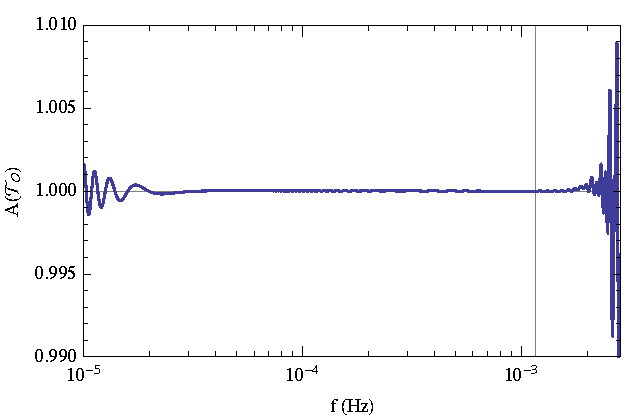
\includegraphics[width=.48\linewidth]{plots/LISAtransferM1e7dOamp.pdf}
  \hspace{0.2cm}
  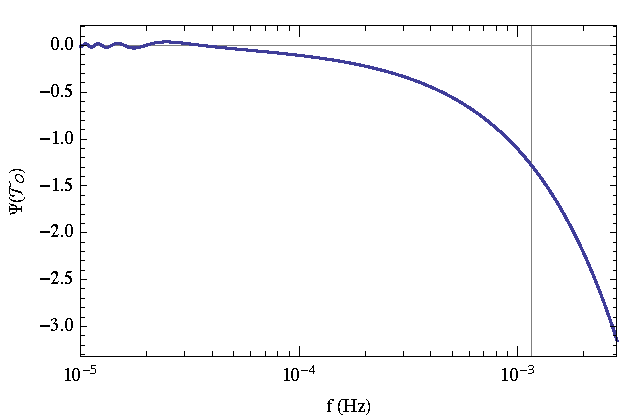
\includegraphics[width=.48\linewidth]{plots/LISAtransferM1e7dOphase.pdf}
  %
  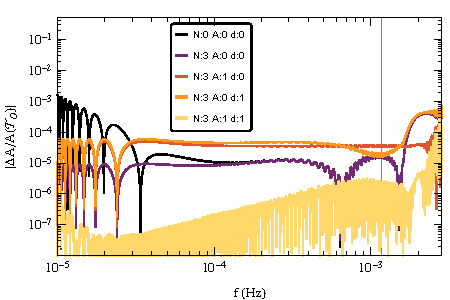
\includegraphics[width=.48\linewidth]{plots/LISAerrorM1e7dOamp.pdf}
  \hspace{0.2cm}
  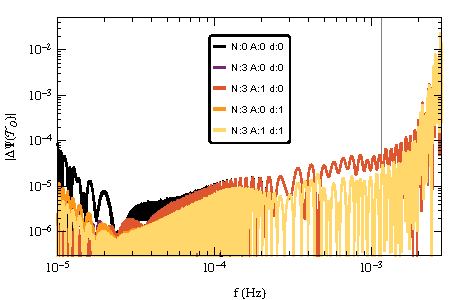
\includegraphics[width=.48\linewidth]{plots/LISAerrorM1e7dOphase.pdf}
  \caption{Error in the transfer function for the orbital delay $d_{O}$, for $M=10^{7} \Msol$.}
  \label{fig:LISAerrorM1e7orb}
\end{figure*}

\begin{figure*}
  \centering
  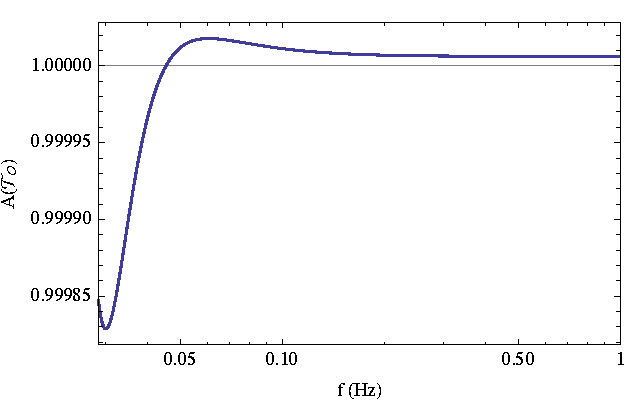
\includegraphics[width=.48\linewidth]{plots/LISAtransferM1e2dOamp.pdf}
  \hspace{0.2cm}
  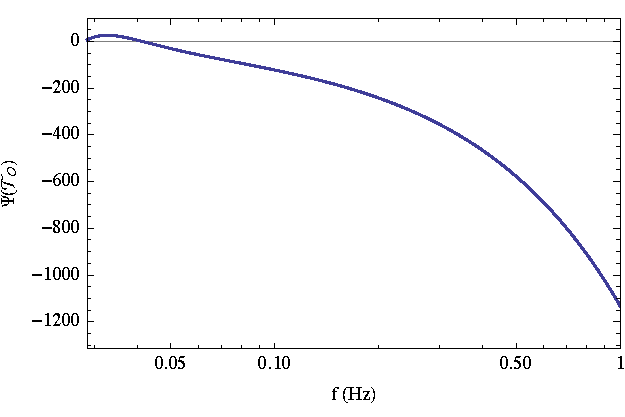
\includegraphics[width=.48\linewidth]{plots/LISAtransferM1e2dOphase.pdf}
  %
  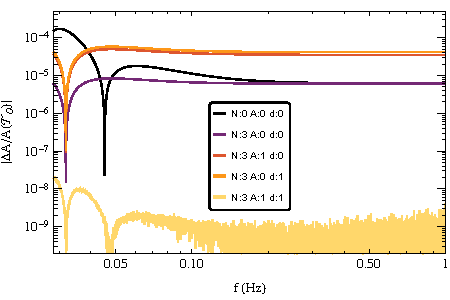
\includegraphics[width=.48\linewidth]{plots/LISAerrorM1e2dOamp.pdf}
  \hspace{0.2cm}
  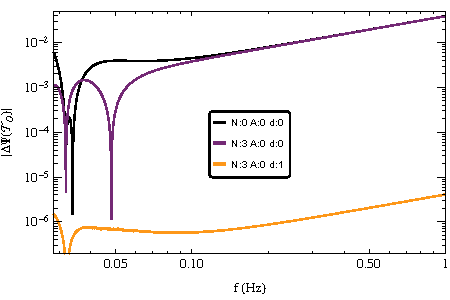
\includegraphics[width=.48\linewidth]{plots/LISAerrorM1e2dOphase.pdf}
  \caption{Transfer function and reconstruction error for the orbital delay $d_{O}$, for $M=10^{2} \Msol$.}
  \label{fig:LISAerrorM1e2orb}
\end{figure*}

\begin{figure}
  \centering
  \includegraphics[width=.98\linewidth]{plots/LISAtransferM1e7y12LReIm.pdf}
  %
  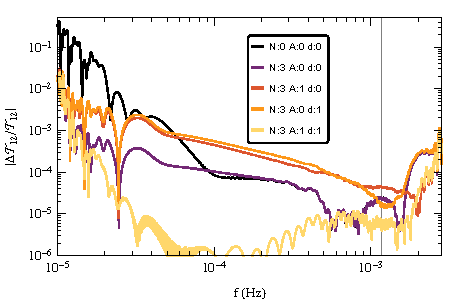
\includegraphics[width=.98\linewidth]{plots/LISAerrorM1e7y12L.pdf}
  \caption{Error in the transfer function for the basic observable $y_{12}$, for $M=10^{7} \Msol$.}
  \label{fig:LISAerrorM1e7const}
\end{figure}

\begin{figure}
  \centering
  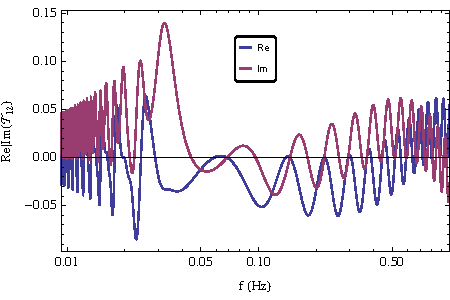
\includegraphics[width=.98\linewidth]{plots/LISAtransferM1e2y12LReIm.pdf}
  %
  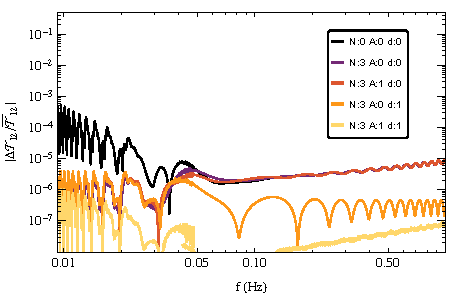
\includegraphics[width=.98\linewidth]{plots/LISAerrorM1e2y12L.pdf}
  \caption{Transfer function and reconstruction error for the basic observable $y_{12}$, for $M=10^{2} \Msol$.}
  \label{fig:LISAerrorM1e2const}
\end{figure}

\SM{[say a word of resampling needed at low and high f, refer to paper PE - discussion section at the end ?]}

%%%%%%%%%%%%%%%%%%%%%%%%%%%%%%%%%%%%

\subsection{Alternative approach for periodic modulations and delays}

In the LISA case, the modulations and delays entering~\eqref{eq:yslr} are periodic, with a period of $f_{0} = 1/\mathrm{yr} \simeq 3.2\times 10^{-8}\mathrm{Hz}$. If the above perturbative formalism cannot be applied, we can still exploit this periodic structure . \SM{[]}
\be
	G(f,t) = \sum_{n} c_{n}(f) e^{-in\Omega_{0}t} \,.
\ee


%%%%%%%%%%%%%%%%%%%%%%%%%%%%%%%%%%%%
%%%%%%%%%%%%%%%%%%%%%%%%%%%%%%%%%%%%

\section{Application to waveforms from precessing binaries}
\label{sec:precession}

\SM{[explain somewhere the fact that the modulation has support for negative f, convolution has support to larger f - pretty important for direct convolution]}

%%%%%%%%%%%%%%%%%%%%%%%%%%%%%%%%%%%%

\subsection{Precession and frame decomposition}
\label{subsec:precdef}

We will now turn to the application of our formalism to the decomposition of signals from precessing binaries. As we already discussed in Sec.~\ref{subsec:modulationPrec}, in the presence of spin components that are not aligned with the orbital angular momentum, an inspiralling binary system will undergo precession of its orbital plane~\cite{Apostolatos+94, Kidder95}. This is a crucial effect to be taken into account in the modelling of such signals.

As proposed by several authors~\cite{BCV03b, BCPTV05, Schmidt+10, OShaughnessy+11, Boyle+11}, if one performs the mode decomposition of the waveform~\eqref{eq:defmodes} not in a fixed inertial frame but rather in a time-dependent, rotating frame that follows the plane of the orbit, it is possible to restore much of the structure of a non-precessing waveform. In particular, one recovers qualitatively the hierarchy of mode amplitudes that prevails for non-precessing systems, with the modes $h_{22}$ and $h_{2,-2}$ being dominant.

We define $(\alpha, \beta, \gamma)$ are the Euler angles relating the precessing frame to the inertial frame in the $(z,y,z)$ convention. The $z$ axis of the inertial frame is chosen to be the direction of $\bm{J}$, the total angular momentum, which is almost constant\footnote{Except in the cases of transitional precession~\cite{Apostolatos+94}, where for high mass ratios and large antialigned spins the orbital angular momentum and the spin can almost cancel each other.}. The first two angles, $\alpha$ and $\beta$, are the two spherical angles tracking the direction of dominant radiation reaction, which during the inspiral follows essentially the normal to the orbital plane. The last angle $\gamma$ parametrizes the remaining freedom of rotation around this radiation axis. An important element of the construction of the precessing frame is the fixing of this third degree of freedom, for which we use the minimal rotation condition~\cite{Boyle+11}
\be\label{eq:gammadot}
	\dot{\gamma} = -\dot{\alpha}\cos \beta \,.
\ee
Quite generically, and in particular in the case of simple precession~\cite{Apostolatos+94, Kidder95} but also in the model we will take for the post-merger precession, the radiation axis precesses on a cone around the direction of $\bm{J}$, with $\alpha$ increasing, while $\beta$, the opening angle of the precession cone, is slowly varying.

The modes in the inertial frame $h_{\ell m}^{\rm I}$ and the modes in the precessing frame $h_{\ell m}^{\rm P}$ are then related by~\cite{Goldberg+67}
\begin{subequations}
\label{eq:wignerrot}
\begin{align}
	h_{\ell m}^{\rm I} = \sum\limits_{m=-\ell}^{\ell} \calD^{\ell *}_{mm'} (\alpha,\beta,\gamma) h_{\ell m'}^{\rm P} \,, \\
	h_{\ell m}^{\rm P} = \sum\limits_{m=-\ell}^{\ell} \calD^{\ell }_{m'm} (\alpha,\beta,\gamma) h_{\ell m'}^{\rm I} \,,
\end{align}
\end{subequations}
where the coefficients $\calD^{\ell}_{mm'}$ are given by Wigner D-matrices~\cite{} \SM{[C]}, which take the expression
\be\label{eq:defWignerD}
	\calD^{\ell}_{mm'} (\alpha, \beta, \gamma) = e^{im \alpha} d^{\ell}_{mm'}(\beta) e^{im' \gamma}\,,
\ee
where the Wigner d-matrix $d^{\ell}_{mm'}(\beta)$ takes the form of a polynomial in $\cos (\beta/2)$, $\sin (\beta/2)$, and acts as an amplitude for the modulation function. We refer to App.~\ref{app:wigner} for explicit expressions.

An important qualitative observation is that, for small to moderate opening angles, the modulation functions show a clear hierarchy in amplitude. This situation is quite generic, since large misalignments between $\bm{J}$ and $\bm{\ell}$ can only be reached with large spins and large mass ratios. From the explicit expressions~\eqref{} \SM{[R]} and~\eqref{} \SM{[R]}, one can see that $d^{\ell}_{mm'}(\beta)$ is greatly suppressed in the limit $\beta \rightarrow 0$ when increasing $|m-m'|$. Intuitively, this means that, in the limit of a small misalignment between frames, the rotation produces mainly mode contributions with the same mode number. Similarly, when $\beta$ is constant or slowly varying, \eqref{eq:gammadot} gives $\gamma \simeq - \alpha \cos\beta$, and we have $\calD^{\ell *}_{mm'} (\alpha, \beta, \gamma) \propto e^{i(m' \cos\beta - m) \alpha}$ with $\cos\beta \simeq 1$ for small $\beta$. This shows that the modulation for $m=m'$ has a suppressed phase, while increasing $|m-m'|$ increases the magnitude of the modulation phase. Thus, modulation functions for distant mode contributions (for instance from the $h^{\rm P}_{22}$ mode all the way to the $h^{\rm I}_{2,-2}$ mode) have larger phase evolutions, but smaller amplitudes.

The relations~\eqref{eq:wignerrot} do not mix different values of $\ell$. Furthermore, rotations leave invariant the combined square amplitude $\calA_{\ell}$ for each $\ell$, as well as the total square amplitude:
\be
	\calA^{2} = \sum\limits_{\ell \geq 2}\calA_{\ell}^{2} = \sum\limits_{\ell \geq 2}\sum\limits_{m=-\ell}^{\ell} |h_{\ell m}|^{2} \,.
\ee
One can therefore use these amplitudes (in our case, limited to $\ell = 2$) to define a frame-independent peak amplitude of the precessing waveform.

Several constructions for the precessing frame have been proposed~\cite{} \SM{[C]}. In the following, we will use a co-precessing frame based on the dominant eigenvector of the matrix representing the action of the angular momentum operator acting on the waveform modes, proposed in~\cite{OShaughnessy+11} (see App.~\ref{app:wigner} for more details \SM{[R]}).

When approximating the precessing-frame waveform by a non-precessing one, one can use the assumption (exactly valid for non-precessing systems, see~\eqref{eq:symmetryhlminusm} \SM{[R]})
\be\label{eq:approxsymmetryhlminusm}
	h^{\rm P}_{\ell,-m} \simeq (-1)^{\ell} h^{\rm P*}_{\ell,m} \,.
\ee
Similarly, for Fourier-domain models, one can neglect either the negative or positive frequency band in the Fourier transform of precessing-frame modes (as in~\eqref{eq:zeronegativef})
\begin{align}\label{eq:approxzeronegativef}
	\tilde{h}_{\ell m}^{\rm P} (f) &\simeq 0 \text{ for } f<0, \; m>0 \nn\,,\\
	\tilde{h}_{\ell m}^{\rm P} (f) &\simeq 0 \text{ for } f>0, \; m<0 \,,
\end{align}
and neglect altogether the $m=0$ modes, $\tilde{h}_{\ell 0}^{\rm P} (f) \simeq 0$.

We will introduce mode-by-mode transfer functions $\calT^{\ell}_{mm'}$,
\be\label{eq:defprectransfer}
	\mathrm{FT} \left[ \calD^{\ell *}_{mm'} (\alpha,\beta,\gamma) h_{\ell m'}^{\rm P} \right] (f) \equiv \calT^{\ell}_{mm'}(f) \tilde{h}_{\ell m'}^{\rm P} (f)
\ee
such that the complete Fourier-domain inertial-frame waveform will be given as the sum of these individual mode contributions,
\be\label{eq:defprechIsum}
	\tilde{h}_{\ell m}^{\rm I} (f) = \sum\limits_{m'=-\ell}^{\ell} \calT^{\ell}_{mm'}(f) \tilde{h}_{\ell m'}^{\rm P} (f) \,.
\ee

When using the assumptions~\eqref{eq:approxsymmetryhlminusm}-\eqref{eq:approxzeronegativef}, one can derive a symmetry relation in the transfer functions themselves. From the explicit expression of the Wigner matrices, we have indeed (see App.~\ref{app:wigner})
\be
	\calD^{\ell *}_{-m,-m'} = (-1)^{m+m'}\calD^{\ell}_{mm'} \,.
\ee
Since for a function $g$ we have in general for its conjugate
\be
	\mathrm{FT}[g^{*}](f) = \tilde{g}(-f)^{*} \,,
\ee
we can write, using~\eqref{eq:approxsymmetryhlminusm},
\be
	\mathrm{FT}[\calD^{\ell *}_{mm'} h_{\ell m'}^{\rm P}](-f)^{*} = (-1)^{\ell+m+m'} \mathrm{FT}[\calD^{\ell *}_{-m,-m'} h_{\ell, -m'}^{\rm P}](f) \,,
\ee
or, for transfer functions,
\be
	\calT^{\ell}_{mm'}(f) = (-1)^{m+m'} \calT^{\ell *}_{-m,-m'}(-f) \,.
\ee
This means that such a model is required to cover only the positive frequency band and the values $m'>0$, the negative frequencies being deduced from
\begin{align}
	\tilde{h}^{\rm I}_{\ell m}(f) &= \sum_{m'>0} \calT^{\ell}_{mm'}(f) \tilde{h}^{\rm P}_{\ell, m'}(f) \text{ for } f>0 \,, \nn\\
	\tilde{h}^{\rm I}_{\ell m}(f) &= \sum_{m'>0} (-1)^{\ell+m+m'} \calT^{\ell *}_{-m,m'}(-f) \tilde{h}^{\rm P *}_{\ell, m'}(-f) \text{ for } f<0 \,.
\end{align}
When including only the leading harmonic $h^{\rm P}_{22}$ in the precessing-frame waveform (as is done for instance in PhenomP~\cite{Hannam+13}), we have for $f<0$
\begin{subequations}
\begin{align}
	\calT^{2}_{m,-2}(f) &= (-1)^{m} \calT^{\ell *}_{-m,2}(-f) \,, \\
	\tilde{h}^{\rm I}_{2 m}(f) &= (-1)^{m} \tilde{h}^{\rm I *}_{2,-m}(-f) \,. \label{eq:symmetryhIfor22only}
\end{align}
\end{subequations}
In general, when including a superposition of modes with different values of $m'$ in the model (for instance, the modes $h^{\rm P}_{22}$ and $h^{\rm P}_{21}$), this symmetry exists only at the level of the mode contributions, and there is no relation such as~\eqref{eq:symmetryhIfor22only}  at the level of $\tilde{h}^{\rm I}_{\ell m}$, as the complete mode reconstruction includes factors $(-1)^{\ell+m+m'}$ in the sum.

In the notation of our formalism of Sec.~\ref{sec:formalism}, 
\be\label{eq:defmodulationprec}
	s(t) = F(t) h(t) \,,
\ee
with $s$ being a mode contribution to $h^{\rm I}_{\ell m}$, $h$ one of the precessing-frame modes $h^{\rm P}_{\ell m'}$, and the modulation $F$ being a Wigner matrix $\calD^{\ell *}_{mm'}$. In the absence of delays, the convolution with a frequency-dependent kernel~\eqref{eq:FDkernel} becomes a simple convolution in the Fourier-domain,
\be\label{eq:convolution}
	\tilde{s} (f) = \int \ud f' \, \tilde{h}(f-f') \tilde{F} (f') \,.
\ee
Our objective is therefore to compute these convolution integrals to obtain the Fourier-domain transfer functions $\calT^{\ell}_{mm'}$. We note an important point about the structure of these comvolution integrals. In presence of the usual behaviour of precession around an almost constant $\bm{J}$, $\alpha$ is monotonously increasing and the modulation functions have the phase evolution $\calD^{\ell *}_{mm'} (\alpha, \beta, \gamma) \propto e^{i(m' \cos\beta - m) \alpha}$. For the 22 mode in the P-frame, $m'=2$, the coefficient of $\alpha$ is close to $0$ for small $\beta$ for $m=2$, and increasingly positive as we go down from $m=1$ to $m=-2$. In our Fourier convention~\eqref{eq:defFT}, the Fourier transforms $\tilde{F}$ thus have most of their support on negative frequencies. This means that the support of the convolution integral~\eqref{eq:convolution} extends to the right side for $\tilde{h}$, i.e. $f-f' > f$. This point will become important when considering the high-frequency part of the signal.

\subsection{Previous approaches}
\label{subsec:precpreviousapproaches}

The above decomposition~\eqref{eq:wignerrot}, and simplifying assumptions~\eqref{eq:approxsymmetryhlminusm}-\eqref{eq:approxzeronegativef} for the precessing-frame waveform, have been widely used for the existing models of waveforms from precessing binaries. For the inspiral phase of the SEOBNRv3 model~\cite{Pan+13,BTB16}, the frame is assumed to follow the instantaneous orbital plane and the waveform in this frame is represented by a spin-aligned expression, with spin-aligned components that are left to vary according to the precessing dynamics. The ringdown phase of the signal is treated differently, the waveform being first rotated back to an inertial frame and then matched to a superposition of quasi-normal modes in this final frame. The PhenomP model~\cite{Hannam+13} uses the decomposition~\eqref{eq:wignerrot} above (although directly in the Fourier domain, as we will detail below) with a precessing-frame waveform given by a spin-aligned PhenomD waveform~\cite{Khan+15,Husa+15}. The SUA waveforms~\cite{KCY14,Chatziioannou+16,Chatziioannou+17}, focused on the inspiral phase, also use the decomposition~\eqref{eq:wignerrot} and a post-Newtonian non-precessing model for the modes $h_{\ell m}^{\rm P}$.

To account for previous approaches to the problem of producing precessing waveforms directly in the Fourier domain, avoiding the use of a FFT \SM{[check acronym]}, it is useful to introduce schematically three levels of approximation (dropping the mode indices):
\begin{itemize}
	\item unstable SPA: $\calT(f) \tilde{h}^{\rm P}(f) = \mathrm{SPA}\left[ \calD^{*} h^{\rm P} \right](f)$,
	\item SPA, $0^{\text{th}}$-order SUA, PhenomP: $\calT(f) = \calD^{*}(\tfSPA) $,
	\item SUA: $\calT(f) = \frac{1}{2} \sum\limits_{k} a_{k} \calD^{*}(\tfSPA \pm k \Tf^{\rm SPA})$.
\end{itemize}

In the first option, one applies directly the SPA, as described in Sec.~\ref{subsec:SPA}, to the product of the modulation and the signal. This is known (see e.g.~\cite{KCY13}) to lead to possible pathologies, since the prefactor $1/\sqrt{\ddot{\phi}_{\rm prec}}$ can blow up due the precessing contributions to the phase, and is not used in waveform modelling.

The second option corresponds to simply multiplying the Fourier-domain signal by the modulation function evaluated at the time $\tfSPA$ as defined in~\eqref{eq:deftfSPA}. In the SUA formalism of Ref.~\cite{KCY14}, this amounts to using a stencil reduced to a single point, i.e. using $a_{0,0} = 1$ in~\eqref{} \SM{[R]}. It is equivalent to the leading order of our formalism, as explained in Sec.~\ref{} \SM{[R]}, with the difference that we use a more general definition of $t_{f}$ (see~\eqref{eq:deftf}) that extends through the merger and ringdown. \SM{[Mention O'Shaugnessy single-spin FD waveforms]}. The PhenomP model~\cite{Hannam+13} implictly uses this level of approximation, although with the notable difference that a frequency-based expression of the modulation is used, allowing to cover the whole frequency band. The precessing-frame evolution is modelled using post-Newtonian expressions for the Euler angles $(\alpha^{\rm PN}, \beta^{\rm PN}, \gamma^{\rm PN}) (\omega)$, that are obtained as functions of the orbital frequency $\omega$ in the limit of a small opening angle of the precession cone and at the spin-orbit level~\cite{Hannam+13} (see also~\cite{BBF11, MBBB13}). Using the SPA-inspired correspondence~\eqref{} \SM{[R]} between the orbital and Fourier-domain frequency, one then writes 
\be\label{eq:precPhenomP}
	\calT^{\ell}_{mm'}(f) = \calD^{\ell *}_{mm'}(\alpha^{\rm PN}, \beta^{\rm PN}, \gamma^{\rm PN}) \left( \omega=\pi f\right) \,.
\ee
When the SPA is valid for the underlying signal $h^{\rm P}_{\ell m}$, the condition $\omega = \pi f$ is equivalent by definition to $t=t^{\rm SPA}_{f}$, but writing things in terms of frequency gives an effective prescription that can cover the whole Fourier-domain frequency band, including the merger and ringdown. Note that this procedure amounts to using PN \SM{[check acronym]} results outside of their range of validity, since in the merger-ringdown phase both the PN perturbative treatment and the SPA approximation break down. In particular, seen as a function of time, $\omega^{\rm PN}(t)$ blows up at merger. In practice, one finds however that the frequency-based expressions~\eqref{eq:precPhenomP} are mildly varying as a function of frequency, and the agreement of the model with numerical relativity waveforms is good~\cite{} \SM{[C]}. 

In the SUA formalism proposed in~\cite{} \SM{[C]}, one extends the SPA to incorporate the leading-order correction during the inspiral phase. The transfer function is then computed by evaluating the modulation on a stencil of times centered around the time-of-frequency given by the SPA, following 
\begin{widetext}
\be
	\calT(f) = \frac{1}{2} \sum\limits_{k=0}^{N} a_{N,k} \left[\calD^{\ell *}_{mm'}(\tfSPA + k \Tf^{\rm SPA}) + \calD^{\ell *}_{mm'}(\tfSPA - k \Tf^{\rm SPA}) \right] \,.
\ee
\end{widetext}
The definition of $\Tf^{\rm SPA}$ was given in~\ref{} \SM{[R]}. As described in Sec.~\ref{} \SM{[R]}, this approach is equivalent to our formalism when keeping only the quadratic phase correction, but is a priori limited to the inspiral phase of the signal through the definitions of the times $t^{\rm SPA}_{f}$ and $T^{\rm SPA}_{f}$. For inspiral waveforms, Ref.~\cite{} \SM{[C]} showed that this treatment improves the accuracy with respect to the local approximation.

The time-domain SEOB~\cite{} \SM{[C]} model includes the modes $h^{\rm P}_{2m}$ with $|m|=2$ and $|m|=1$ for the inspiral, and the ringdown constructed in the inertial frame contains a superposition of all modes $h^{\rm I}_{2 m}$ by construction. In the PhenomP~\cite{} \SM{[C]} model, only the dominant harmonics $h^{\rm P}_{22}$ and $h^{\rm P}_{2,-2}$ were included in the precessing-frame waveform. The SUA~\cite{} \SM{[C]} model can be constructed using any PN non-precessing model for an inspiral-only waveform, including higher harmonics. \SM{[Check what is implemented in LAL ? HM or not ?]}

\subsection{Simplified model for precessing IMR waveforms}
\label{subsec:precmodel}

\SM{[qualify how bad the model is with respect to full NR]}

\SM{[explain shortcomings of pure SEOB in post-merger, problem of smoothness]}

We now present our toy model for IMR waveforms of precessing binaries, which we will use in the following to illustrate the accuracy of the Fourier-domain transfer functions at various orders of approximation. Since our purpose in this article is not to propose a full-fledged waveform model, but rather to investigate wether the formalism of Sec.~\ref{sec:formalism} is relevant to tackle the merger part of the signals, and wether its application reduces the errors in the reconstruction of transfer functions, we will allow for a number of idealizations and simplifications in this toy model.

Although the frame decomposition and precessing-frame prescription is well understood for the inspiral, where the precessing frame roughly follows the orbital plane of the binary (see~\ref{} \SM{[R]}), we wish to investigate the merger and ringdown part of the signal as well, and need a way to extend this intuitive picture.

\SM{[acronym QNM]}

For this extension, one needs to define a precessing frame after merger, when the orbital plane has lost any meaning. This can be done naturally when using a frame prescription that is not tied to the dynamics but directly extracted from the gravitational waveform, such as~\eqref{} \SM{[R]}. Investigating the post-merger behaviour of this frame requires numerical relativity simulations of precessing binaries. Ref.~\cite{} \SM{[C]} proposed a qualitative model where the frame vector essentially keeps precessing around the final $\bm{J}$, but transitions to a faster precession rate. More precisely, they observe that the interpretation of the post-merger waveform as an excitation of a superposition of quasinormal modes suggests that the frame should evolve according to the difference of the leading QNM frequencies. In their simulations, they find indeed a precession rate around the final total angular momentum $\hat{\bm{J}}_{\rm final}$, asymptoting to the angular velocity
\be\label{eq:OmegaframeQNM}
	\Omega_{\rm frame} = \omega_{220}^{\rm QNM} - \omega_{210}^{\rm QNM} \,.
\ee
The behaviour of the opening angle of the precessing cone $\beta$, however, is harder to interpret. Although it usually shows some transition at merger (to a lower value), it does not show an exponential decay as the interpretation above would suggest. We found that overall this picture is at least qualitatively correct for the precessing waveforms	 currently available in the SXS catalog. \SM{[allowed to make such a vague statement about catalogue waveforms ?]}

Note however that this model should be taken with caution, since the parameter space currently accessible to numerical simulations of precessing systems is limited in spin mass ratio. The behaviour of systems with a close-to-extremal remnant spin largely remains to be explored. In addition, systems with large mass ratios and large anti-aligned spins on the primary black hole can have a total angular momentum dominated by the primary spin instead of the orbital angular momentum (e.g. in the case of transitional precession~\cite{} \SM{[C]}). This can lead to the remnant spin being anti-aligned with respect to the precessing frame axis prior to merger. This could conceivably lead to a different structure in the excitation of the quasi-nomal modes, and to a qualitatively different frame behaviour. Assessing the limits of validity of this model would require a more extensive coverage of the parameter space by numerical relativity simulations and would go beyond the scope our present study. 

The basic ingredients of our model \SM{[apologize for the Frankenstein-ism !]} will be: \SM{[move most of all this to an appendix]}
\begin{itemize}
	\item PhenomD~\cite{} \SM{[C]} for the precessing-frame waveform;
	\item SEOB for Euler angles during the inspiral;
	\item an effective extension of the Euler angles post-merger based on~\eqref{eq:OmegaframeQNM}.
\end{itemize}
For the precessing-frame waveform, in keeping with the approximation~\eqref{} \SM{[R]} for the precessing-frame waveform we will use a slightly modified version of the PhenomD waveform model~\cite{} \SM{[C]}, a Fourier-domain model that covers the inpiral, merger and ringdown for binaries with generic aligned spins. The waveform is produced as piecewise analytical expressions\footnote{The PhenomD model is publicly available in the LIGO Algortitm Library (LAL).}. We limit ourselves to the dominant harmonics $h^{\rm P}_{22}$ and $h^{\rm P}_{2,-2}$ (see~\cite{} \SM{[C]} for a recent extension of the model to include higher harmonics). Using a Fourier-domain approximant that is smooth by construction avoids the problems arising from the tapering time-domain waveforms, as we will detail below, and will allow us to easily take Fourier-domain derivatives of the waveform. Since the PhenomD amplitude and phase are only of class $C^{1}$, to avoid spurious discontinuities we introduce decaying corrective terms of the form $(f-f_{\rm join})^{2} e^{-\lambda(f-f_{\rm join})^{2}}$ on each side of $f_{\rm join}$, the junction frequency between two bands. Here $\lambda$ is a large parameter ensuring that the modification remains local. The modificiations have very little effect overall but artificially enforce the continuity of second derivatives.

For the frame trajectory in the inspiral phase, we extract the dominant-eigenvector frame as defined in~\eqref{} \SM{[R]} from an SEOB waveform. Since the SEOB waveform is constructed by using the instantaneous orbital plane of the dynamics as the precessing frame, the frame extraction procedure simply gives back the orbital plane (except very close to merger where the waveform starts to smoothly transition to the post-merger QNM superposition). The frame thus presents oscillatory features of small amplitude at the orbital timescale, due to the nutation of the orbital plane \cite{} \SM{[C]}.

For the extension of the frame trajectory post-merger, we do not rely on the PhenomP procedure as it is merely effective. Furthermore, we found that the ringdown attachment procedure, as implemented in SEOB, leads to frame trajectories that show oscillations in all the Euler angles when the spins are anti-aligned. These oscillations increase in amplitude as the spins go to larger misalignments, and are already present well beneath the regime of transitional precession. Since we checked that the qualitative behaviour~\eqref{eq:OmegaframeQNM} holds rather well for numerical relativity simulations in regions of the parameter space where SEOB starts to show these oscillations, and since the SEOB post-merger ringdown attachment is an effective representation, we chose to use an artificial post-merger extension of the frame, following
\be\label{eq:alphaQNM}
	\alpha_{\rm post-merger}(t) = \alpha(t_{\rm peak}) + (\omega_{220}^{\rm QNM} - \omega_{210}^{\rm QNM})(t-t_{\rm peak}) \,.
\ee
Since we do not have yet a quantitative model of the behaviour of the opening angle of the precessing cone $\beta$, we simply set it to a constant value post-merger, taken to be its value at merger. The third Euler angle $\gamma$ is extended using the minimal rotation condition~\eqref{} \SM{[R]}. For the QNM frequencies as a function of the final spin, we use values tabulated in Ref.~\cite{} \SM{[C]}. The final spin is taken to be the same as in the SEOB code~\cite{} \SM{[C]}, where the final-spin fit formula of Ref.~\cite{} \SM{[C]}, built for spin-aligned systems, is applied to the spin components \SM{[check that and complete]}. Our simple extension is an idealization, especially for the angle $\beta$, and is not to be considered quantitatively accurate. However, it allows us to capture what we believe to be the dominant post-merger behaviour, in the sense that the frame is set to rotate with a velocity of the right order of magnitude, which is crucial for us since we want to investigate how the separation between the orbital (or $h^{\rm P}_{\ell m}$) timescale and the precessing timescale is challenged post-merger. We show in Fig~\ref{} the frequencies $\omega_{220}^{\rm QNM}$, $\omega_{210}^{\rm QNM}$ and their difference $\Omega_{\rm frame}$. The behaviour for near-to-extremal spin of the remnant would require more exploration, as the QNM frequencies vary a lot when approaching extramality. \SM{[add plot of QNM frequency and frequency diff according to final spin]}.  Fig.~\ref{fig:prectoymodel} presents a comparison of the frame trajectory at merger for the SEOB, NR waveforms and for our model. The example catalog waveform is SXS:BBH:0058~\cite{} \SM{[C]}, which presents a rather high mass ratio of $q=5$, with a single spin in-plane of $\chi_{1} = 0.5$. The NR and SEOB post-merger frames disagree mainly due to a different value of the final spin $\chi_{f}$\footnote{Work is underway to update the fit formulas used to compute $\chi_{f}$ in the SEOB code, which is expected to reduce these disagreement~\cite{}. \SM{[C]} \SM{[work in preparation by SEOB people, essentially already done]}}, which leads to a different $\Omega_{\rm frame}$. Given their different value of $\chi_{f}$, however, both agree with the qualitative prescription~\eqref{eq:OmegaframeQNM}. The oscillations developing after $t\sim 50 M$ occur in a regime where the overall waveform amplitude has decayed to small values, and are not important in that regard. Our model follows well the SEOB behaviour for $\alpha$ and $\gamma$, but departs more for $\beta$ as it ignores its variation at merger. 

To combine our various waveform ingredients, we first ensure that the PhenomD and SEOB waveforms are aligned in time, by performing an inverse Fourier transform of PhenomD and applying a time shift to both waveforms so that the peak amplitude occurs at $t=0$ (taken for SEOB to be the $\ell=2$ combined square amplitude~\eqref{}, and for PhenomD just the peak of the 22 mode for PhenomD). We apply to the resulting frame trajectory a Gaussian filtering following the same procedure as the one used for numerical-relativity surrogate of Ref.~\cite{} \SM{[]}: the scale of the filter is set to a fixed width in waveform phase \SM{[detail what we used exactly]}. This filtering ensures a continuity of the modulation function and their derivatives at the point of attachment. It also eliminates the nutation of the frame at the orbital timescale, which are generically less pronounced in the frame extracted following~\eqref{} \SM{[R]} from numerical relativity simulations than for the normal to the orbital plane.

Note an important caveat of our approach: the application of the perturbative formalism presented in Sec.~\ref{sec:formalism} relies on the smoothness of both the time-domain modulation and the Fourier-domain signal. For the time-domain modulation, the assumption of the separation of timescales~\eqref{} \SM{[R]} relies on the identification of a characeteristic frequency $\Omega_{\rm prec}$, which is based on the time derivative of $F$. It is always possible to add and remove arbitrarily small oscillations in $F$ that would give arbitrarily large contributions to its derivatives, hence affecting any local computation of $\Omega_{\rm prec}$. One can consider that our approach is to be applied to such a slowly varying approximation of $F$, that can be obtained by filtering away rapidly-varying, small-amplitude features. However, we should keep in mind that any smoothing procedure could possibly eliminate  some information present in the original waveforms.

For the smoothness of the signal in the Fourier domain, one has to keep in mind that, for waveforms computed starting with a time-domain waveform, Gibbs oscillations can be mitigated by properly tapering the waveform in time domain before performing the FFT, however taking Fourier-domain derivatives magnifies this oscillations, to the point that they would dominate among others the timescale $\Tf$ (unless one takes much longer waveforms to push this problem to lower frequencies). This is avoided in our case by working with a pure Fourier-domain PhenomD waveform that is smooth by construction, but would become important if one were to apply our formalism to the FFT of NR or SEOB waveforms.

Another caveat is that for the precessing-frame waveform, the assumption~\eqref{eq:approxsymmetryhlminusm} is only approximate. Mode asymmetries are present in the late inspiral and merger phases of precessing binaries, as shown by numerical relativity simulations (see e.g.~\cite{} \SM{[C]}). These asymmetries play a role in the emission of linear momentum and in the resulting kick of the black hole remnant, and they also result in amplitude and phase variations on the orbital timescale.

In the following, we will illustrate our formalism by applying it to three examples. The parameters of these example cases are summarized in Table~\ref{table:precparams}. We consider a mass ratio of $q=4$, close-to-maximal spins of $\chi_{1} = \chi_{2} = 0.95$, and vary both spins misalignmnent angles to be $\pi/6$ (close to spin-aligned), $\pi/2$ (spins in the plane) and $5\pi/6$ (close to anti-aligned spins). Table~\ref{table:precparams} also shows the remnant spins that are internally computed in both the SEOB and the PhenomD/PhenomP codes, as well as the QNM frequencies and the resulting frame precession frequency $\Omega_{\rm frame}$. Note that the case $--$ shows a larger variation in the direction of $\bm{J}$, and the spin of the remnant is almost 0, due to the fact that the spin is large and antialigned, with a large mass ratio. This example therefore serves the purpose of lying at the edge of validity of the picture of standard precession along a cone around an almost-fixed direction, and the standard hierarchy between mode contributions is not valid in this case. \SM{[soundness of trajectories, particularly in this case, are to be checked again]}

\begin{figure*}
  \centering
  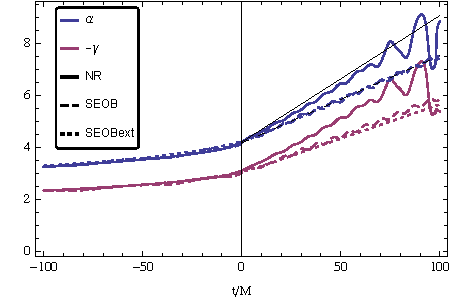
\includegraphics[width=.45\linewidth]{plots/eulerSXS0058alphagamma.pdf}
  \hspace{0.2cm}
  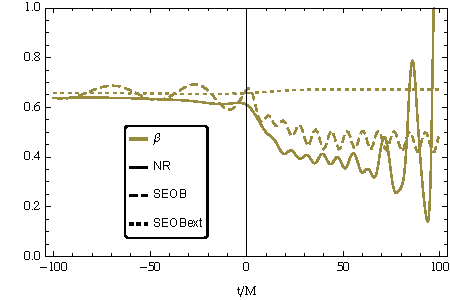
\includegraphics[width=.45\linewidth]{plots/eulerSXS0058beta.pdf}
  \caption{Evolution of Euler angles $(\alpha, \beta, \gamma)$ near merger for the example waveform SXS:BBH:0058~\cite{} \SM{[C]}. Full, dashed and dotted lines represent the NR, SEOB and extended SEOB waveforms respectively. The vertical line at $t=0$ indicates the time of merger. In the left panel the full and dashed black lines indicate the asymptotic behaviour~\eqref{eq:OmegaframeQNM} for the rotation of the frame around the direction of the final $\bm{J}$. The difference between NR and SEOB there is due to the value of the final spin, with $\chi_{f}^{\rm NR} = 0.54$ and $\chi_{f}^{\rm SEOB} = 0.42$, which leads to a different $\Omega_{\rm frame}$. In the right panel, $\beta$ is asymptotically constant in our toy model. \SM{[Add amplitude/$\omega$ plots comparing NR/SEOB, and possibly PhenomD for the 22 mode ? Add Euler angles produced by IFFT of PhenomP ?]}}
  \label{fig:prectoymodel}
\end{figure*}

%\begin{figure*}
%  \centering
%  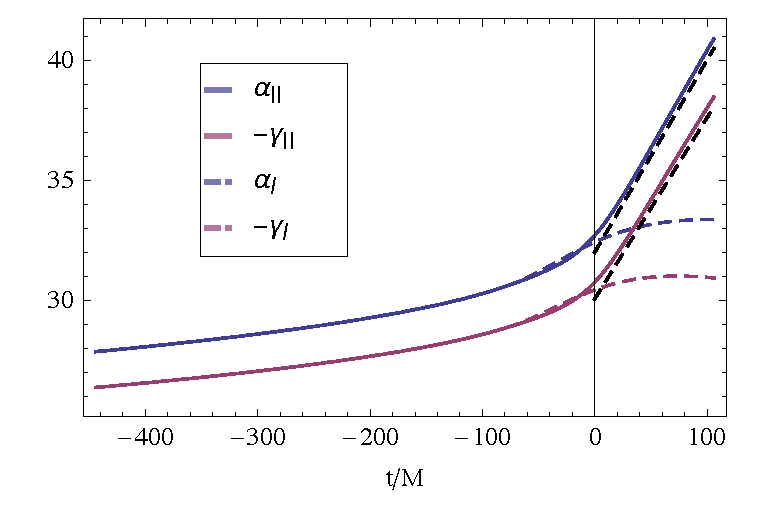
\includegraphics[width=.48\linewidth]{plots/prectoymodelalphagamma.pdf}
%  \hspace{0.2cm}
%  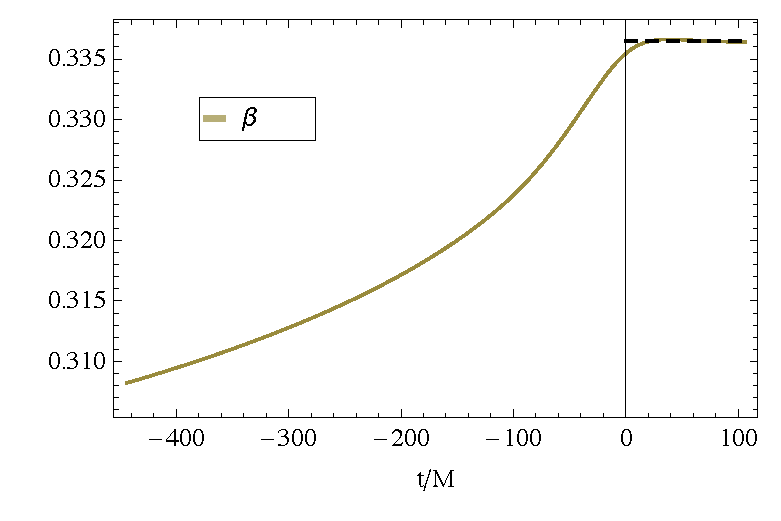
\includegraphics[width=.48\linewidth]{plots/prectoymodelbeta.pdf}
%  \caption{Evolution of Euler angles $(\alpha, \beta, \gamma)$ for our two toy models. Dashed lines represent Case I and solid lines Case II. The vertical line indicates the time of merger. In the left panel the dashed black lines indicate the enforced asymptotic behaviour in Case II, where the frame rotates with constant angular velocity $\omega_{220} -\omega_{210}$. In the right panel, $\beta$ is asymptotically constant.}
%  \label{fig:prectoymodel}
%\end{figure*}

\SM{[Check the mismatch for $--$ between Jf from dynamics and chif used in SEOB internals to do the ringdown attachment - check that the frame trajectory makes sense by comparing to orbital plane.]}

%In Eq.~\eqref{eq:defmodulationprec} above, the modulation function $F$ evolves on the precessional timescale, which evolves throughout the inspiral. The separation between the precessional timescale and the orbital timescale will be crucial for our analysis. In the limit of low frequencies, we will see in Sec.~\ref{} below that, although these timescales become more and more separated, the decrease in the chirping rate gives raise to a corrective contribution that does not vanish in this limit. In the other limit, as the system gets close to merger, the separation of timescales becomes weaker, and we will explore in Sec.~\ref{} the application of our formalism to the merger and ringdown phase.

\begin{table}[t]
\begin{ruledtabular}\caption{Parameters of of the three example cases that we use to illustrate our formalism. The three cases differ by their spin alignment angles $\theta_{A} = \bm{\chi}_{A} \cdot \hat{\bm{L}}_{i}$, the spins being in the orbital plane, almost aligned and almost anti-aligned. The table gives also the final spins magnitudes (for SEOB as well as PhenomD for comparison), angles between the initial and final angular momenta $\theta(\bm{J}_{i}, \bm{J}_{f})$, as well as QNM frequencies and frame rotation velocity used for the post-merger extension. \SM{[To be updated with longer waveforms, 10Hz 10Msol.]} \SM{[add misalignment angles $(\ell, \bm{J}_{i})$]}}\label{table:precparams}
%\begin{tabular}{C{.2\columnwidth}C{.24\columnwidth}C{.15\columnwidth}}
\begin{tabular}{ccccccc}\label{table:precexamples}
	$f_{\rm min}$ & $ M_{\rm min} $ & $q$ & $\chi_{1}$ & $\chi_{2}$ & $ \phi_{1} $ & $ \phi_{2} $ \\
	\hline
	$20\mathrm{Hz}$ & $20\Msol$ & $ 4.0 $ & $ 0.95 $ & $ 0.95 $ & $0$ & $\pi/2$ \\
	\hline\hline
	Case && ++ && $pp$ && $--$ \\
	\hline
	$\theta_{1}$ && $\pi/6$ && $\pi/2$ && $5\pi/6$ \\
	$\theta_{2}$ && $\pi/6$ && $\pi/2$ && $5\pi/6$ \\
	\hline
	$\chi_{f}$ && $0.89$ && $0.50$ && $0.02$ \\
	$\chi_{f}^{\rm Ph}$ && $0.90$ && $0.47$ && $0.002$ \\
	$\theta(\bm{J}_{i}, \bm{J}_{f})$ && $0.02$ && $0.04$ && $0.27$ \\
	$M \omega_{220}^{\rm QNM}$ && $0.66$ && $0.47$ && $0.377$ \\
	$M \omega_{210}^{\rm QNM}$ && $0.51$ && $0.42$ && $0.375$ \\
	$M \Omega_{\rm frame}$ && $0.15$ && $0.04$ && $0.002$ \\
\end{tabular}
\end{ruledtabular}
\end{table}

%\begin{table}[t]
%\begin{ruledtabular}\caption{Parameters of the three example cases that we use to illustrate our formalism.}\label{table:precparams}
%%\begin{tabular}{C{.2\columnwidth}C{.24\columnwidth}C{.15\columnwidth}}
%\begin{tabular}{cccc}
%	Case & pp & $++$ & $--$ \\
%	\hline
%	$q$ & $4.0$ & $4.0$ & $4.0$ \\
%	$\chi_{1}$ & $0.95$ & $0.95$ & $0.95$ \\
%	$\chi_{2}$ & $0.95$ & $0.95$ & $0.95$ \\
%	$\theta_{1}$ & $\pi/2$ & $\pi/6$ & $5\pi/6$ \\
%	$\theta_{2}$ & $\pi/2$ & $\pi/6$ & $5\pi/6$ \\
%	$\phi_{2}$ & $0.0$ & $0.0$ & $0.0$ \\
%	$\phi_{2}$ & $\pi/2$ & $\pi/2$ & $\pi/2$
%\end{tabular}
%\end{ruledtabular}
%\end{table}

\SM{[We could add plots of the 3 frame trajectories, and of the FD transfer functions in Amp/Phase form. But the trajectories are not very informative except for - - (where our model might not be very solid) and for showing oscillations in $\beta$. The reconstruction errors plots already show the amplitude of the modes themselves, giving an idea of the hierarchy; what is the missing is the phase in Tlmmp, which is not very informative.]}

%\begin{figure*}
%  \centering
%  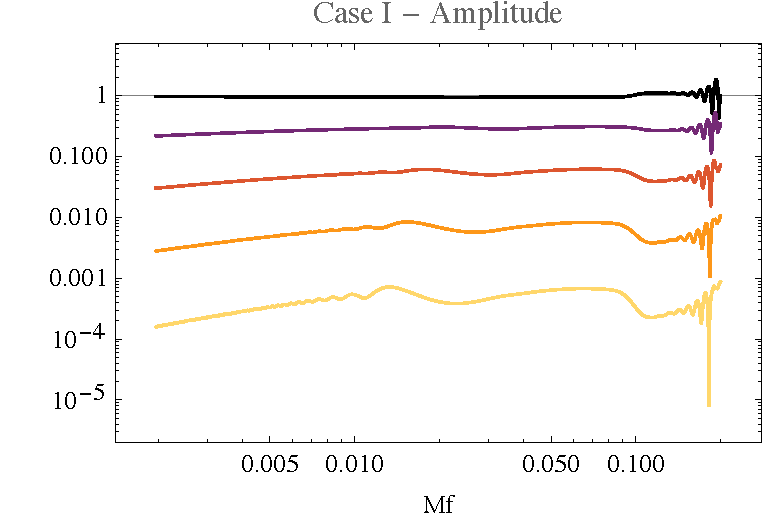
\includegraphics[width=.48\linewidth]{plots/prectransferAcaseI.pdf}
%  \hspace{0.2cm}
%  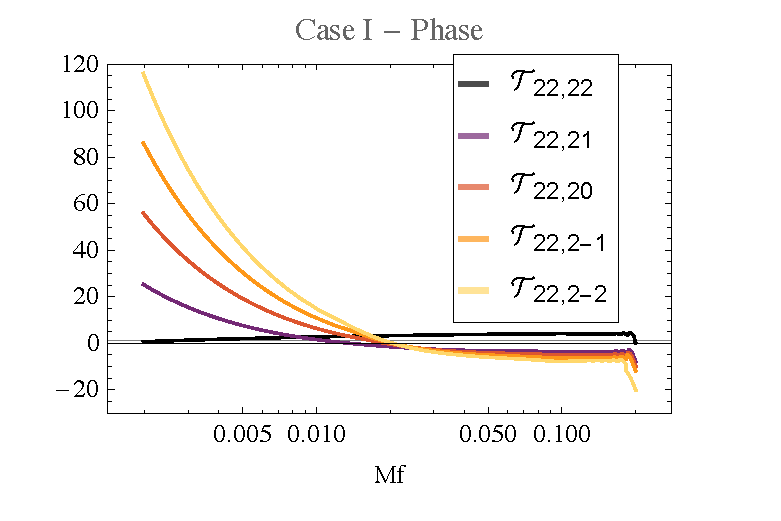
\includegraphics[width=.48\linewidth]{plots/prectransferPsicaseI.pdf}
%  %
%  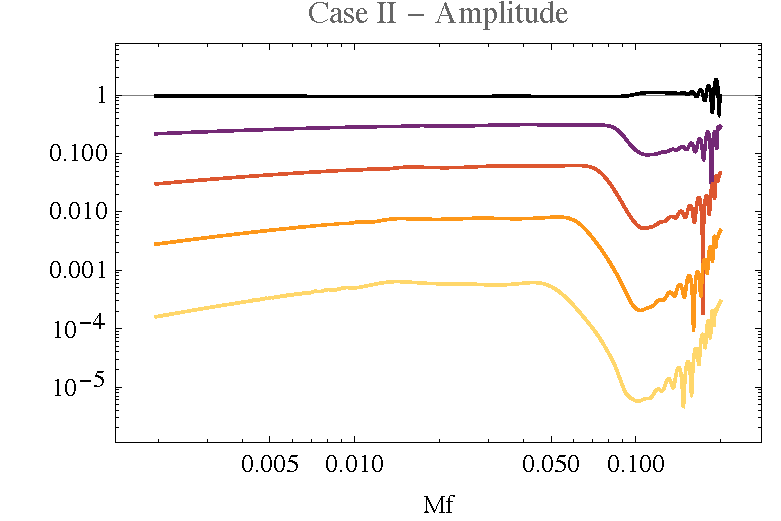
\includegraphics[width=.48\linewidth]{plots/prectransferAcaseII.pdf}
%  \hspace{0.2cm}
%  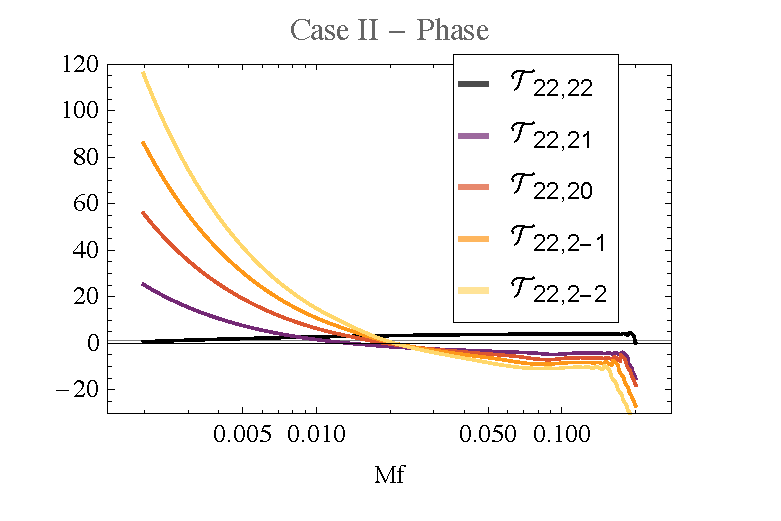
\includegraphics[width=.48\linewidth]{plots/prectransferPsicaseII.pdf}  
%  \caption{Amplitude and phase of the Fourier-domain transfer fonctions $\calT_{22,2m'}$ as defined in~\eqref{eq:defTlmlmp} for individual mode contributions. The left panels show the amplitude and the right panels the phase.}
%  \label{fig:prectransfer}
%\end{figure*}

%%%%%%%%%%%%%%%%%%%%%%%%%%%%%%%%%%%%

\subsection{Estimates for the magnitude of higher-order corrections}
\label{subsec:sizecorrPrec}

\SM{[Add full expressions for the $\epsilon$ quantities]}

\SM{[justify somewhere smallness of cubic-in-phase term]}

We now investigate the magnitude of higher-order corrections in the case of precessing binaries, using the error estimates $\epsilon_{\Psi 2}$, $\epsilon_{A1}$ and $\epsilon_{A 2}$ defined in~\eqref{eq:deffom}. We would like to stress that these figures are to be understood as merely order-of-magnitude estimates, since they compute the error of each approximation by gauging the magnitude of the first corrective term in a Taylor series. In particular, they rely on computing derivatives of the time-domain modulation, which can be sensitive to oscillatory features.

First, we would like to stress that the modulation functions $\calD^{\ell *}_{mm'}$. As shown in~\ref{app:Wigner}, their phase dependence is. \SM{[complete]}

For the inspiral phase of the dynamics, one can read the quantities $\epsilon_{\Psi 2}$, $\epsilon_{A1}$ and $\epsilon_{A 2}$ from the outcome of post-Newtonian computations. To obtain a qualitative picture of the timescales involved, here we will consider the most simple setting for precession in the post-Newtonian framework: at leading PN order and for a single-spin system, both the orbital angular momentum $\bm{L}$ and the spin vector $\bm{S}$ undergo what is called simple precession around the total angular momentum, $\bm{J}$ (see e.g.~\cite{Apostolatos+94, Kidder95}). By neglecting the slow evolution of the orbit under radiation reaction, ignoring higher-order corrections that are quadratic and higher in the spins, and orbit-averaging the precession equations (thus eliminating nutations in the precession of the orbital plane, which occur at the orbital timescale), the trajectories of $\bm{L}$ and $\bm{S}$ become cones around the direction of $\bm{J}$, with a constant precession velocity $\Omega_{\rm prec}$ that we will use to define the timescale of variations of the modulation functions $F$. Note that the presence of two spins complicates the evolution of the system, but the picture of a precession cone for $\bm{\ell}$ remains approximately valid (see~\cite{} \SM{[C]} for a classification of the morphologies of precessing trajectories).

In the following, we will use the notation \SM{[use M instead of m]} $m=m_{1}+m_{2}$, $\nu=m_{1}m_{2}/m^{2}$, $\delta = (m_{1}-m_{2})/m$, $|\bm{S}_{A}|=Gm_{A}^{2} \chi_{A}$ for $A=1,2$. We take the convention $m_{1} \geq m_{2}$. We define $\bm{\ell}$ as the unit vector normal to the orbital plane, and assume that only the more massive object has a spin, so that $\bm{S}_{2} = 0$. A factor $c$ is scaled out of the spins so that $S_{A} = G m_{A}^{2} \chi$, with $\chi$ the dimensionless spin between $0$ and $1$ for Kerr black holes. We will use the notation $v = (G m \omega/c^{3})^{1/3}$ with $\omega$ the orbital frequency, which is equivalent to the frequency-domain definition $v=(G \pi m f/c^{3})^{1/3}$ when the SPA applies. \SM{[Check redundancy with notations of previous sections]} The Newtonian order orbital angular momentum is $\bm{L} = L_{N} \bm{\ell}$, with
\be\label{eq:defLN}
	L_{N} = \frac{G m^{2} \nu}{c v} \,.
\ee
Since we neglect radiation reaction, $\bm{J}$ is treated a constant that we use to set the z-axis so that $\bm{J} = J \bm{e}_{z}$, and we decompose the spin in its aligned and perpendicular components as $\bm{S}_{1} = S_{1}^{z} \bm{e}_{z} + \bm{S}_{1}^{\perp}$. At leading order, the precession equations read
\begin{align}
	\dot{\bm{S}}_{1} &= \bm{\Omega}_{1} \times \bm{S}_{1} \,, \nn\\
	\dot{\bm{\ell}} &= - \frac{1}{c L_{N}}  \dot{\bm{S}}_{1}\,, \nn\\
\end{align}
with the spin precession velocity \cite{} \SM{[C]}
\be
	\bm{\Omega}_{1} = \Omega_{1} \bm{\ell} = \frac{c^{3}}{G m} \left( \frac{3}{4} + \frac{\nu}{2} - \frac{3\delta}{4} \right) v^{5} \bm{\ell} \,.
\ee
which is formally a 1PN quantity. Decomposing the vectors in their in-plane component and projection on $z$, and using $\delta^{2} = 1-4\nu$ to make explicit the overall scaling in $\nu$, we obtain for the frame precession velocity (defined such that $\dot{\alpha} = \Omega_{\rm prec}$)
\be
	\Omega_{\rm prec} = \frac{c^{4}}{G^{2} m^{3}} \frac{7+\delta}{2(1+\delta)} v^{6} J\,.
\ee
For convenience, we will use the notation
\begin{subequations}
\begin{align}
	\Lambda &\equiv \frac{7+\delta}{4(1+\delta)} \,, \\
	\xi &\equiv 1 + \frac{v S_{1}^{z}}{G m^{2} \nu} \,.
\end{align}
\end{subequations}
$\Lambda$ is a mass ratio-dependent factor chosen to be of order 1, varying from $7/4$ for equal masses to $1$ in the test-mass limit. The factor $\xi$ shows how the contribution of the spin to the total angular momentum affects the precession rate. With this notation,
\be\label{eq:Omegaprec}
	\Omega_{\rm prec} = \frac{2c^{3} \nu}{G m} \Lambda \xi v^{5} \,.
\ee
If precession effects are in general larger for larger mass ratios, as the precession cones widens, the overall scaling of $\nu$ in~\eqref{eq:Omegaprec} above ($\Lambda$ has a mild variation with masses, which is also decreasing with increasing mass ratio) shows that, as long as the orbital angular momentum still dominates the spin, high mass ratio systems have also a slower precession rate.

We now turn to the Euler angles and modulation functions $\calD^{\ell *}_{mm'}(\alpha, \beta, \gamma)$, given explicitly in~\eqref{eq:defWignerD}. In the case of simple precession, the opening angle of the precession cone, $\beta$, evolves solely due to radiation reaction. If we treat it as a constant, the minimal rotation condition relates $\gamma$ to $\alpha$ by $\gamma  = -\alpha \cos \beta$ (up to a constant), and the only variable part of the modulation functions~\eqref{} \SM{[R]} are the phases. The constant rate of rotation around $\bm{J}$ translates into $\dot{\alpha} = \Omega_{\rm prec}$. From the closure relation $\bm{J} = \bm{L} + \bm{S}_{1}$, we have
\be\label{eq:betaconst}
	\cos \beta = \sqrt{1 - \left( \frac{S_{1}^{\perp}}{c L_{N}} \right)^{2}}\,.
\ee
For each mode contribution $\calD^{\ell *}_{mm'}$, we have
\be
	\calD^{\ell *}_{mm'} (\alpha, \beta, \gamma) \propto e^{i(m' \cos\beta - m) \alpha}
\ee
which gives an additional geometric factors of $(m' \cos\beta - m)$.
Under our assumptions of simple precession, ignoring radiation reaction, and using the leading-order expressions~\eqref{} \SM{[R]} for the Fourier-domain timescales, we finally obtain the following error estimates for individual modes:
\begin{subequations}
\begin{align}
	\epsilon_{\Psi 2} &= \frac{5\nu}{96} \Lambda^{2} \xi^{2} (m' \cos\beta - m)^{2} v^{-1} \,, \\
	\epsilon_{A 1} &=  \frac{7\nu}{6} \Lambda \xi |m' \cos\beta - m| v^{2} \,, \\
	\epsilon_{A 2} &= \frac{91 \nu^{2}}{72} \Lambda^{2} \xi^{2} (m' \cos\beta - m)^{2} v^{4} \,.
\end{align}
\end{subequations}
As noted in Section~\ref{} \SM{[R]}, $\epsilon_{\Psi 2}$ has a factor $v^{-1}$, formally at $-0.5$PN order, which means that the relative size of this correction grows towards smaller frequencies, away from merger. Remember however that the opening angle of the precession cone, giving the overall normalization for precession effects in the waveform, also goes to 0 as $v$ in that limit. The amplitude error estimates $\epsilon_{A1}$, $\epsilon_{A2}$, by contrast, have the more usual behaviour of PN corrections (of order 1PN and 2PN respectively) growing towards merger. The geometric factors $(m' \cos\beta - m)$ show that higher $|m-m'|$ mode contributions are harder to model, with larger $\epsilon$, although they also have smaller amplitudes for small $\beta$. The overall $\nu$ scalings indicate a better separation of timescales for larger mass ratio systems. These expressions also show that, since the total angular momentum appear as a factor in $\Omega_{\rm prec}$, higher-order corrections will be larger for spin-aligned systems than for antialigned spins \SM{[language: antialigned or anti-aligned ?]}, an effect that becomes significant for large mass ratios. Note that when $\xi$ gets close to 0, it means that the system is in the transitional precession range, with the spin of the primary compensating the orbital angular momentum, and our analysis based on simple precession is not valid anymore.

The previous expressions for the error estimate only aim at providing a crude order-of-magnitude picture. We now present a more complete numerical computation of these quantities for our post-merger extended precession model presented in Sec.~\ref{subsec:precmodel}, for the three examples summarized in Table.~\ref{table:precexamples}. Here and in the following we present only the $h^{\rm I}_{2 m}$ mode contributions induced by $h^{\rm P}_{22}$, knowing that the ones induced by $h^{\rm P}_{2,-2}$ can be deduced from~\eqref{} \SM{[R]}. We compute the Fourier-domain based timescales $\Tf$, $T_{A1}$ and $T_{A2}$ from the analytic derivatives of the PhenomD phase and amplitude (modified to be of class $C^{2}$). The time derivatives of the time-domain modulation are computed from an interpolating cubic spline. The results are shown in Fig.~\ref{fig:fomprec}, using the frequency at merger, shown by the vertical lines, to give an idea of the separation between the inspiral and post-merger phases. The first two cases, $++$ and $pp$, have \SM{[come back to this after having checked trajectories]} the usual behaviour of precession on a cone, with a larger opening angle for $pp$ due to the larger in-plane spin components. After merger, the case $++$ shows a much faster frame rotation than the $pp$ case, as shown by the values of $\Omega_{\rm frame}$ in Table~\ref{table:precexamples}, due to the larger remnant spin that incorporates the aligned spin components. The case $--$ is qualitatively different, with a larger variation of $\bm{J}$ in direction, and a large and varying $\beta$. Since the $\epsilon$ quantities are the magnitude of the first or second term in a Taylor series, we will take $\epsilon \sim 1$ as an indication of the breakdown of a perturbative treatment. We recall an important point about Fig.~\ref{fig:fomprec}: since the error estimates are computed on a mode-by-mode basis and normalized by the transfer function for this mode, the amplitude hierarchy between mode contributions is erased here. What is plotted is an error estimate in relative sense, and one should keep in mind that higher $|m-m'|$ modes, which we will find harder to model accurately, can be very subdominant in the final waveform.

The resulting magnitude of the error estimates in Fig.~\ref{fig:fomprec} is roughly in agreement with the PN-inspired computation~\ref{eq:} \SM{[R]} above for the inspiral \SM{[check if the PN is quantitatively ok -- overlay it on the plot ?]}. For the inspiral, the magnitude of the quadratic phase term $\epsilon_{\Psi 2}$ has a negative slope $v^{-1}=(Mf)^{-1/3}$ \SM{[check the slope on the figure]}, with a clear hierarchy that is due to the prefactor of $\alpha$ in the phase of the modulation, as explained above. This hierarchy is not respected for $--$. The mode $m=2$, the most important to model once the amplitudes are refactored in, is mainly in the perturbative regime, but we see that the perturbative treatment can be challenged for modes $m\leq 0$ and also for $m=1$ in the case $++$, especially for the post-merger. The amplitude corrections are found to be in the perturbative regime for all cases during the inspiral, however both the $++$ and $pp$ cases show a sharp increase of $\epsilon_{A1}$, $\epsilon_{A2}$ post-merger. The case $--$, with its small remnant spin and mild post-merger frame rotation, shows no such increase.

Overall, the conclusion to be drawn of Fig.~\ref{} is that for the $++$ and $pp$ cases we expect the perturbative approach to be applicable only during the inspiral, with a possible breakdown for the post-merger phase, especially for the case $++$ with its fast post-merger frame rotation. The higher $|m-m'|$ modes are expected to be more challenging to compute accurately, including during the inspiral. To make this picture quantitative, we need a full comparison of the signals processed at different orders of approximation against a numerical Fourier transform, which will be presented in Sec.~\ref{subsec:precerror} below.

\SM{[Pb: scaling of FOM might be dominated here by SS oscillations, notably for 2nd der. ? To check - check also geometric scaling from mode to mode]}

\begin{figure*}
  \centering
  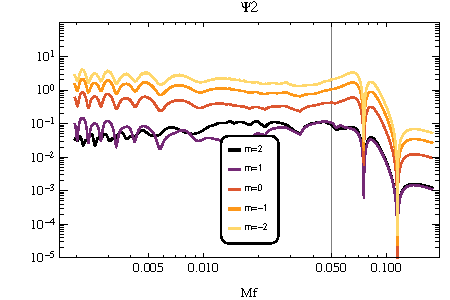
\includegraphics[width=.32\linewidth]{plots/fom_pp_Psi2.pdf}
  \hspace{0cm}
  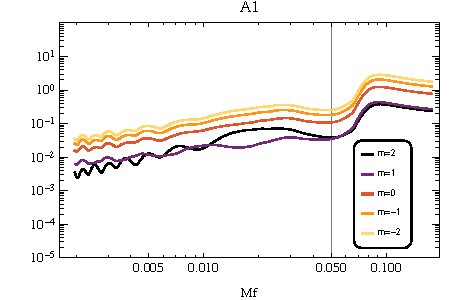
\includegraphics[width=.32\linewidth]{plots/fom_pp_A1.pdf}
  \hspace{0cm}
  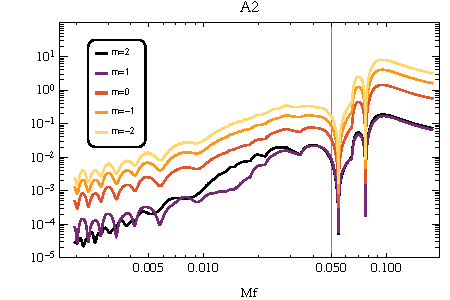
\includegraphics[width=.32\linewidth]{plots/fom_pp_A2.pdf}
  %
  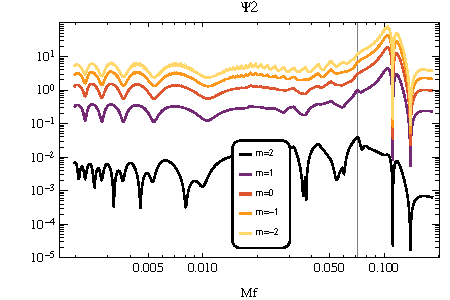
\includegraphics[width=.32\linewidth]{plots/fom_++_Psi2.pdf}
  \hspace{0cm}
  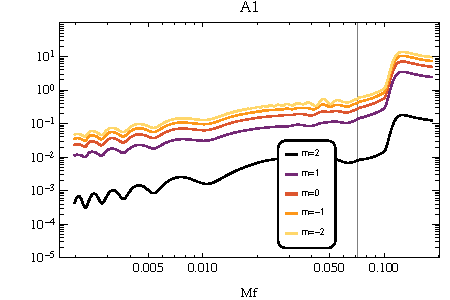
\includegraphics[width=.32\linewidth]{plots/fom_++_A1.pdf}
  \hspace{0cm}
  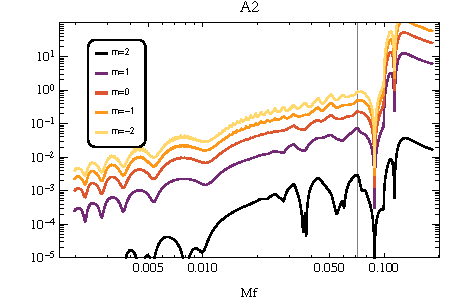
\includegraphics[width=.32\linewidth]{plots/fom_++_A2.pdf}
  %
  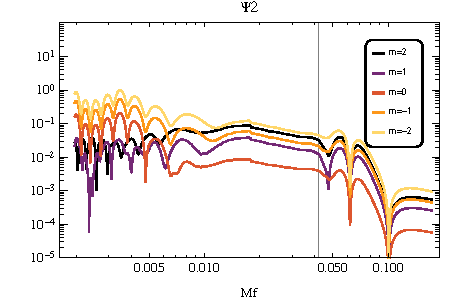
\includegraphics[width=.32\linewidth]{plots/fom_--_Psi2.pdf}
  \hspace{0cm}
  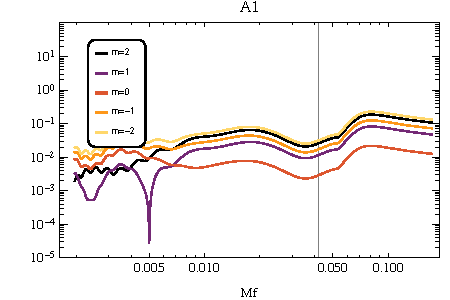
\includegraphics[width=.32\linewidth]{plots/fom_--_A1.pdf}
  \hspace{0cm}
  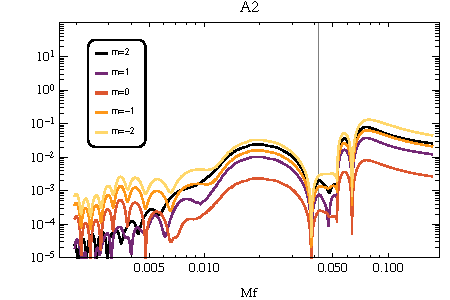
\includegraphics[width=.32\linewidth]{plots/fom_--_A2.pdf}
  \caption{Error estimates of the approximation as defined in~\eqref{eq:deffom} for the precession modulations. \SM{[transpose, compact the columns to share the x axis, fix legends, add horizontal line for $10^{0}$]}}
  \label{fig:fomprec}
\end{figure*}

%\begin{figure*}
%  \centering
%  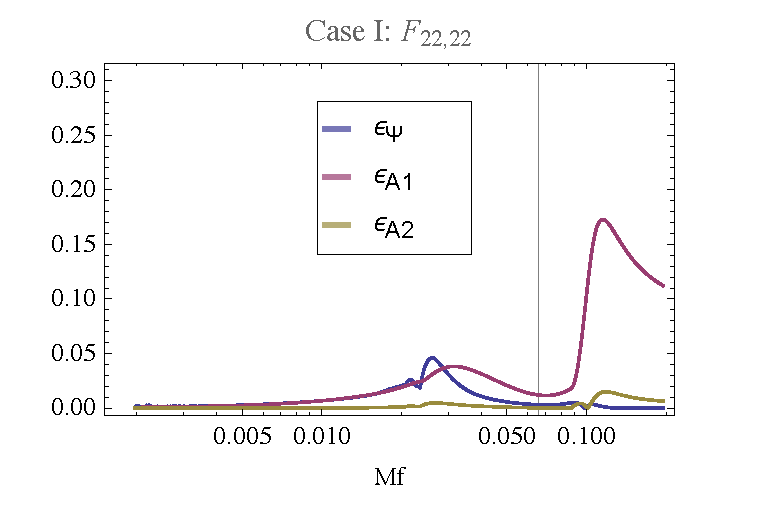
\includegraphics[width=.48\linewidth]{plots/precfom22caseI.pdf}
%  \hspace{0.2cm}
%  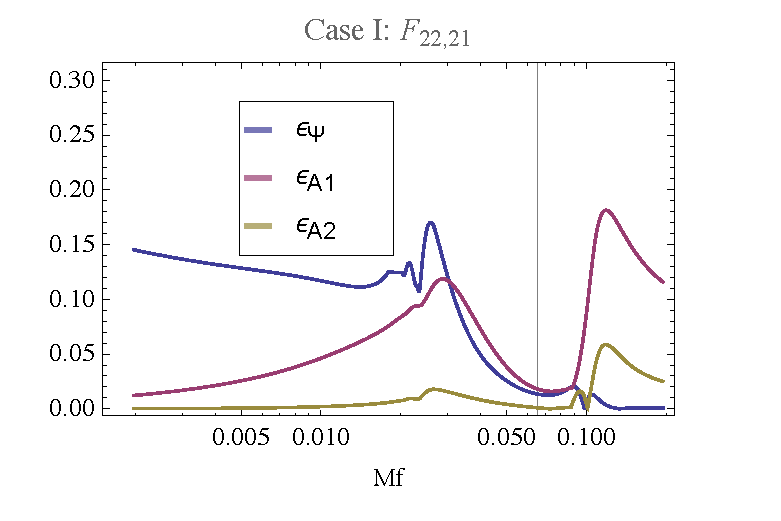
\includegraphics[width=.48\linewidth]{plots/precfom21caseI.pdf}
%  %
%  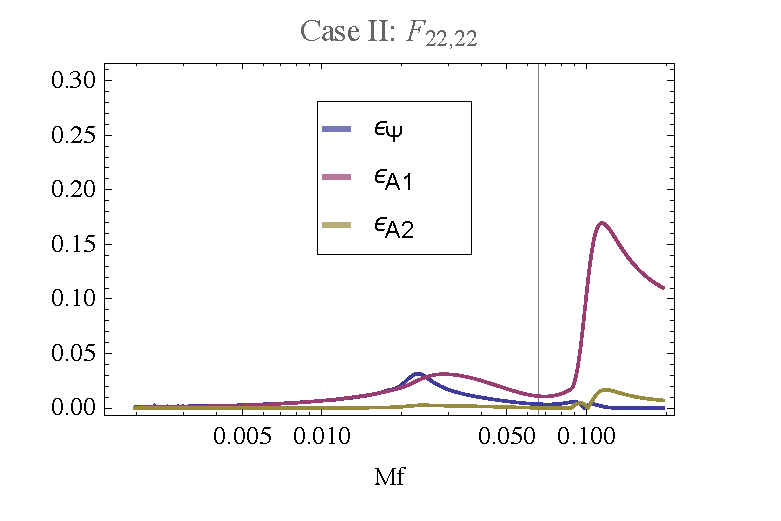
\includegraphics[width=.48\linewidth]{plots/precfom22caseII.pdf}
%  \hspace{0.2cm}
%  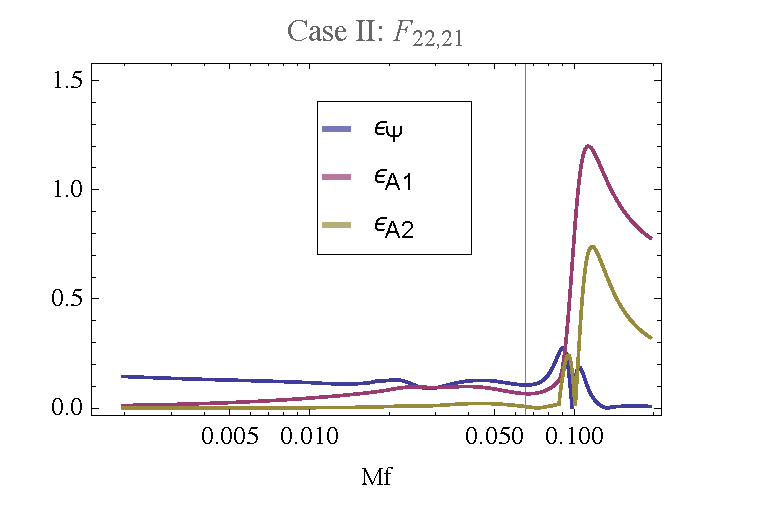
\includegraphics[width=.48\linewidth]{plots/precfom21caseII.pdf}
%  \caption{Figures of merit of the approximation as defined in~\eqref{eq:deffom} for the precession modulations. The precessing-frame waveform is taken to be the $22$ mode of an equal-mass, non-spinning system. The two upper panels show the case where the frame rotation is freezed at merger (Case I), while the two lower panels show the case where it rotates after merger (Case II) (see Sec.~\ref{subsec:precmodel} for their definitions). The left panels show the figures of merit for $F_{22, 22}$, and the right panels for $F_{22, 21}$. The vertical line represents the frequency at merger. The amplitude corrections become non-negligible after merger, and become large enough to challenge a perturbative treatment in Case II for $F_{22,21}$ (notice the change of scale for the lower right panel).}
%  \label{fig:TfTA}
%\end{figure*}

%%%%%%%%%%%%%%%%%%%%%%%%%%%%%%%%%%%%

\subsection{Direct convolution approach for the merger-ringdown phase}
\label{subsec:convolution}

\begin{figure*}
  \centering
  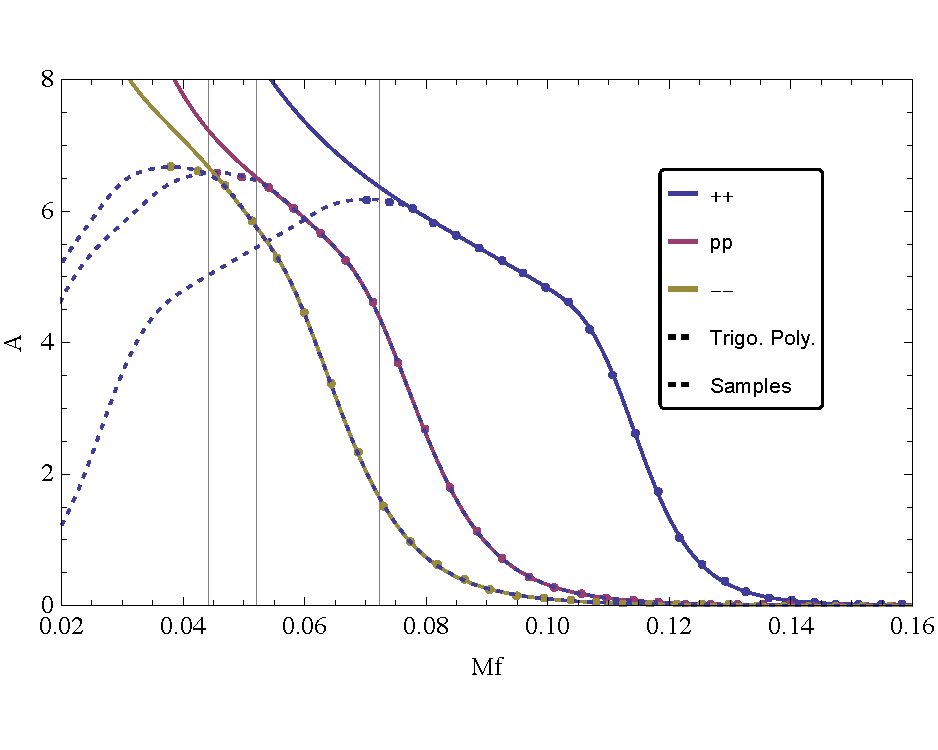
\includegraphics[width=.48\linewidth]{plots/trig_amp.pdf}
  \hspace{0.2cm}
  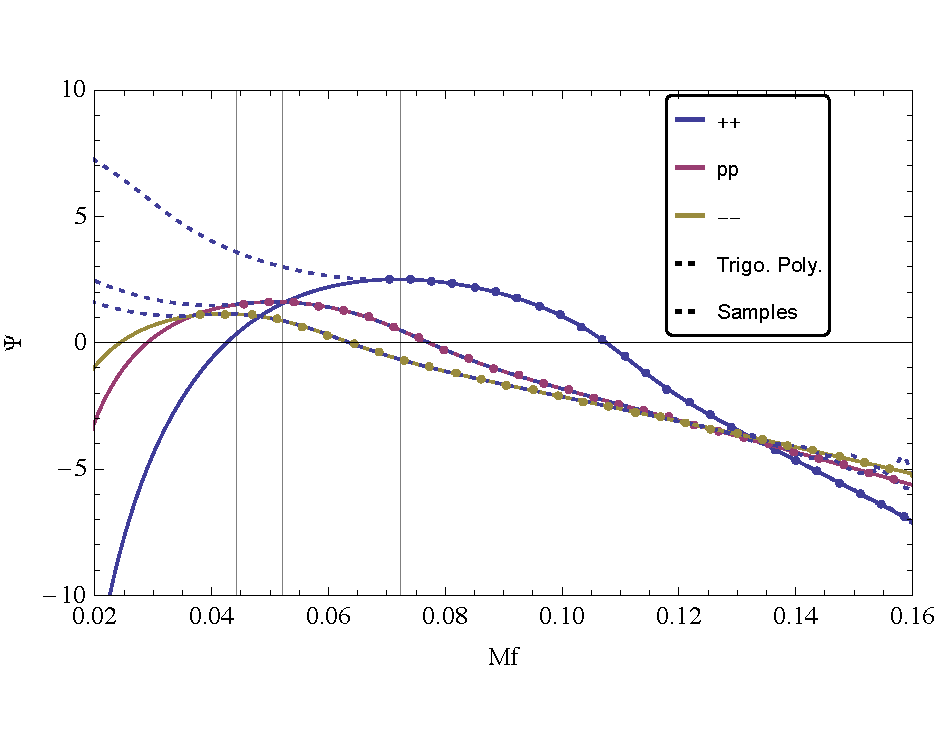
\includegraphics[width=.48\linewidth]{plots/trig_phase.pdf}
  \caption{Amplitude (left panel) and phase (right panel), compared to its trigonometric polynomial representation for the three cases listed in Table~\ref{table:precexamples}. The vertical lines indicate the merger frequencies. \SM{[color for vertical lines at fpeak]}}
  \label{fig:trigopoly}
\end{figure*}

\SM{[possibly move this to the formalism section ? but plots for our three examples]}

As will be shown by Fig.~\ref{} below, although including higher-order amplitude corrections does capture some effects near merger, it is not sufficiently accurate and seems to be too sensitive to the details of the evolution of the modulation $F(t)$ in the merger region. Motivated by this shortcoming of the Taylor-like expansion approach, here we investigate an alternative way of handling the merger-ringdown part of the signal.

Thanks to the separation of timescales between the precessional timescale and the orbital timescale, for suffciently high frequencies the convolution~\eqref{eq:convolution} will have a support that will be entirely comprised in the high-frequency part of the signal $\tilde{h}(f)$, which is rather featureless and slowly varying as a function of $f$. Taking advantage of this smoothness, we will adopt a trigonometric polynomial representation for $\tilde{h}(f)$. For frequencies high enough that the support of the convolution~\eqref{eq:convolution} does not extend beyond the range covered by this trigonometric representation, we will be able to write the result directly as a Discrete Fourier Transform (DFT) with a limited number of samples.

We consider the high-frequency part of the signal above some frequency $f_{0}$, above which the signal has limited amplitude and phase evolution, up to some maximal frequency $f_{\rm max}$ where the Fourier-domain amplitude of the signal has decayed to a negligible level. In practice, we define $f_{\rm knee}$ as the peak of $f^{2}A(f)$, representing the onset of the decay in amplitude, and roughly corresponding to $\omega_{22}^{\rm QNM}/\pi$. We set $f_{0}\equiv 2/3f_{\rm knee}$, which is close to the merger frequency, and $f_{\rm max}$ is chosen so that the amplitude is $10^{-4}$ of the amplitude at $f_{\rm knee}$. We also eliminate a constant and a linear term in the phase by choosing another frequency central to the high-frequency range we want to represent, which we take to be $f_{p} = f_{\rm knee}^{2/3} f_{\rm max}^{1/3}$ with corresponding time $t_{p}\equiv \tf(f_{p})$. Note that the method should only be weakly sensitive to the precise choice of $f_{p}$ and $t_{p}$.

Additionaly, we taper the amplitude to artificially flatten the amplitude at $f_{0}$, at the price of introducing a deviation from the amplitude of the original signal. This tapering is built in practice as the discrete integral of a cosine window function on just the first two samples. We taper to 0 the last three samples before $f_{\rm max}$. To ensure good continuity properties, we perform an artificial symmetrization to a fictitious range $f\in [f_{0} - (f_{\rm max} - f_{0}), f_{0}]$, by imposing symmetric amplitudes and phases about $f_{0}$. Defining $\Delta f \equiv 2 (f_{\rm max} - f_{0})$, we write
\begin{widetext}
\be\label{eq:defhsym}
	\tilde{h}_{\rm sym}(f) = 
	\begin{cases} 
		\exp\left[i \Psi(f_{0}) - 2i\pi (f-f_{0}) t_{p} \right] \tilde{h}(f) \,,  &\text{ for } f \in [f_{0}, f_{0} + \Delta f /2] \\
	\tilde{h}_{\rm sym}(2 f_{0} - f)^{*} \,,  &\text{ for } f \in [f_{0} - \Delta f/2, f_{0}]
	\end{cases}
\ee
\end{widetext}

Next, we build a a trigonometric polynomial representation of $\tilde{h}_{\rm sym }$. This construction is intimately related to the DFT, but we recall it for completeness. For a periodic function $F(x)$ defined on $x\in [x_{0}, x_{0} + \Delta x]$, and represented by $N$ samples $x_{j} = \ov{x} + j \Delta x/N$ (with $N$ chosen to satisfy the Nyquist criterion \SM{[historically should be called Shannon ?]}), we can build a trigonometric interpolant $P(x)$ as
\be
	P(x) = \sum\limits_{k=-M}^{+M} c_{k} e^{2i\pi k \frac{x-x_{0}}{\Delta x}}
\ee
that will satisfy the system $P(x_{j}) = F(x_{j})$ for $j=0,\dots, N-1$. Here we set $M=N/2$ (assuming N is even). The coefficients $c_{k}$ are related to the coefficients of the inverse DFT of the series for $F$. If we set $\omega \equiv e^{2i\pi/N}$ and define
\be
	y_{k} = \frac{1}{N} \sum\limits_{j=0}^{N-1} F(x_{j}) \omega^{jk} \,,
\ee
which is the expression of the inverse DFT in our sign convention~\eqref{eq:defFT}, the coefficients $c_{k}$ are given by
\begin{align}\label{eq:ckyk}
	c_{k} &= y_{k} \text{ for } k=0,\dots, M-1 \,, \nn\\
	c_{k} &= y_{k+N} \text{ for } k=-M+1,\dots, -1 \,, \nn\\
	c_{M} &= c_{-M} = \frac{y_{M}}{2} \,,
\end{align}
where the condition $c_{M} = c_{-M}$ is an arbitrary condition enforced to match the number of degrees of freedom. In practice, we also 0-pad by a factor of 2 to high frequencies. Fig~\ref{fig:convolsymmetrized} shows both the original high-frequency part of the signal and its reconstruction as a trigonometric polynomial.

Now, assuming that we wish to compute~\eqref{eq:convolution} for a frequency $f$ such that the extent of the convolution does not extend beyond $[f_{0}, 2f_{\rm max} - f_{0}]$, we can approximate
\be\label{eq:hsymtrigo}
	\tilde{h}_{\rm sym } (f) \simeq \sum\limits_{k=-M}^{+M} (-1)^{k} c_{k} e^{2i\pi k \frac{f-f_{0}}{\Delta f}} \,,
\ee
where the factor $(-1)^{k}$ comes from the fact that $f_{0}$ is here at the center of the interval. The coefficients $c_{k}$ are built following the rules~\eqref{eq:ckyk} from the inverse DFT coefficients
\be\label{eq:ykDFT}
	y_{k} = \frac{1}{N} \sum\limits_{j=0}^{N-1} \tilde{h}_{\rm sym}\left( f_{0} + \frac{2j - N}{N} \Delta f \right) \omega^{jk} \,.
\ee
When inserting this representation~\eqref{eq:defhsym} and~\eqref{eq:hsymtrigo} into~\eqref{eq:convolution}, we obtain
\begin{align}\label{eq:resultdirectconvol}
	\tilde{s}(f) &= e^{-i \Psi(f_{0})} e^{2i\pi (f-f_{0}) t_{p}} \nn\\
	& \qquad \cdot\sum\limits_{k=-M}^{+M} (-1)^{k} c_{k} e^{2i\pi k \frac{f-f_{0}}{\Delta f}} F(t_{p} + k\delta t) \,, 
\end{align}
where we defined the time sampling $\delta t \equiv 1/\Delta f$. We see that we are left with a DFT-like expression to compute from $N+1$ time samples of the modulation function $F$, centered around $t_{p}$.

The crucial point in this approach is that the convolution integral in~\eqref{eq:convolution} has support mainly on $f'<0$, which means to the right of $f$ in Fig.~\ref{fig:trigopoly} as discussed in Sec.~\ref{subsec:} \SM{[R]}. This means that the trigonometric representation of $\tilde{h}(f)$ can be used to compute the convolution almost all the way down to $f_{0}$, effects of the tapering aside.

In terms of performance, the implementation of~\eqref{eq:ykDFT} and~\eqref{eq:resultdirectconvol} above is expected to have a very reasonable cost. We obtained results with a good accuracy, as shown in Fig.~\ref{fig:trigopoly}, by including $M=64$ samples ($32$ useful samples before 0-padding, $N=128$ samples in total for the artificially symmetrized signal). The calculation described here is done only once for a given waveform and modulation function. The number of samples is of the same order of magnitude as the number of (logarithmically-spaced) frequency samples used to represent the Fourier-domain waveform with its amplitude and phase in the first place, thus the cost is comparable to the Taylor-like approach presented in Sec.~\ref{sec:quadphasedelay} \SM{[R]}.

\SM{[update performance - plots were made with double number of points]}

\SM{[explain what this all means translated in terms of sampling in the time-domain -- better relate this approach to simply IFFT]}

\SM{[for plot illustrating reconstruction trigo of amplitude : what normalization to pick for A FD ?]}

%%%%%%%%%%%%%%%%%%%%%%%%%%%%%%%%%%%%

\subsection{Error control for the Fourier-domain modulation}
\label{subsec:errorsPrec}

We now assess the accuracy of the transfer function computation, applying the formalism of Secs.~\ref{} and \ref{} to our three examples listed in Table~\ref{table:precexamples} and comparing the result to a reference numerical computation.

To numerically compute the transfer functions, we first have to perform an IFFT of our Fourier-domain P-frame waveform, to obtain $h^{\rm P}_{22}$ as a function of time. To mitigate the effect of the necessary tapering of the waveform when computing this numerical inverse Fourier transform, we apply a Planck-window tapering on the range $f\in 16-20 \text{Hz}$, using a total mass of $M=20 \Msol$. \SM{[Update this to $f_{\rm min} = 10\text{Hz}$]}. In parallel, we generate an SEOB waveform with the appropriate length in time. Both are aligned to peak at $t=0$, we build the post-merger extended modulation functions as explained in Sec.~\ref{} \SM{[R]}, and we compute the Fourier-domain modes $h^{\rm I}_{2m}$ with an FFT. The transfer functions are then computed using~\eqref{eq:defprectransfer}.

In the following, we will either present the errors obtained with the formalism of Sec.~\ref{sec:formalism} applied to the whole frequency band, including the merger and ringdown part of the signal, or cover the high-frequency range with the convolution treatment of Sec.~\ref{subsec:convolution}, with a Planckian window on $Mf\in [Mf_{0}, Mf_{\rm knee}]$ for a smooth transition between the two formalisms.

The figures Fig.~\ref{fig:precerrors++}, Fig.~\ref{fig:precerrorspp} and Fig.~\ref{fig:precerrors--} display three successive approximations: $\{\Psi:0,A:0\}$, which is simply the leading-order transfer function~\eqref{eq:transferlocal}, ignoring all the corrections; $\{\Psi:2,A:2\}$, which incorporates both the phase corrections~\eqref{eq:Fresnelstencil}, using a stencil size $N=3$, and the amplitude corrections up to second order in~\eqref{eq:transferfinal}; and $\{\Psi:2,A:2,\text{conv}\}$, which is the same as the previous for the inspiral but uses the convolution formalism of Sec.~\ref{}. They show the Fourier-domain amplitude for each of the modes, both exact and from the reconstruction, the relative errors in amplitude, and the errors in phase. The errors are given in a relative sense, and the amplitude allows to visualize the mode hierarchy, and give an idea of how much the relative errors matter in an absolute sense.

The $++$ case, as expected from the analysis of the previous section, is the most challenging, with large relative errors. Applying higher-order corrections improves the accuracy in the inspiral, but the most difficult modes $m=-1$ and $m=-2$ still show large errors. We also find that higher-order corrections do not reduce the errors in the merger-ringdown region, indicating a breakdown of the perturbative formalism as indicated by Fig.~\ref{fig:fomprec}. Using the convolution treatment improves the main modes $m=2$, $m=1$, but not the most challenging modes $m=-1$ and $m=-2$, which can be seen to depart from the perturbative treatment before the range covered by the convolution. Note however that, as we will show below by computing the full unfaithfulness these large errors for the higher modes do not affect much the full waveform.
\SM{[explain how the convolution formalism fails - convolution support to the right, in low-amp region, not well controlled]}

For the $pp$ case, we find a clearer picture. Errors are increasing to larger $|m-m'|$, higher-order corrections improve the reconstruction but are unsufficient for the merger-ringdown, and the convolution works for all modes on the frequency range where it is applied. The errors at the very high end of the frequency band occur when the overall amplitudes are low, and are therefore unimportant. 

For the $--$ case, the mode hierarchy is not respected, as the frame trajectory does not quite follow the picture of simple precession. The precession velocity is much milder, leading to smaller errors. Apart from some amplitude errors in the merger-ringdown region, we find that in this case even the leading-order treatment gives very reasonable results.

In order to illustrate what these errors really mean for the analysis of GW signals, we also compute the unfaithfulness (or mismatch) between various orders of approximation and the exact, numerical result. This unfaithfulness figure, although giving a simplified view of waveform inaccuracies, is commonly used to quantify disagreements between template families and to compare them to numerical relativity waveforms. For real signals $h_{1}$ and $h_{2}$, one introduces the usual noise-weighted scalar product
\be\label{eq:defoverlap}
	\left( h_{1} | h_{2} \right) = 4\text{Re} \int_{0}^{+\infty} \ud f \frac{\tilde{h}_{1}(f) \tilde{h}_{2}^{*}(f)}{S_{n}(f)} \,,
\ee
with $S_{n}(f)$ the noise power spectral density, for which we use the aLIGO ZDHP noise curve~\cite{} \SM{[R]}.

For spin-aligned waveforms, the unfaithfulness is customarily defined as the normalized overlap~\eqref{eq:defoverlap} above optimized over the time at coalescence and global phase of the signal. In the precessing case, different prescriptions coexist, differing by the extrinsic parameters that are optimized over. Here we adopt the same prescription that was used in the construction of a numerical relativity surrogate model for precessing waveforms~\cite{} \SM{[R]}. We refer to the Appendix.~\SM{[R]} of~\cite{} for more details \SM{[complete a bit here]}.

Here we take our illustrative model of Sec.~\ref{} \SM{[R]} as the reference waveform, thus ignoring the inaccuracy introduced by our approximate treatment of post-merger precession and focusing only on the passage from time-domain to Fourier-domain. We show the unfaithfulness obtained for 3 inclination angles between the line-of-sight and the direction of the final $\bm{J}$, $0$ (face-on), $\pi/3$ and $\pi/2$ (edge-on), using different approximations (note that we consider more options than for the preceding error plots). The total mass ranges from $20\Msol$ (where the inspiral dominates) \SM{[to be updated to $10 \Msol$]} to $400\Msol$ (where the merger-ringdown phase dominates). The symbol $\Psi:n$ with $n=0$ or $n=2$ means that the phase corrections~\eqref{eq:Fresnelstencil} are either ignored or included with a stencil size $N=3$. The symbol $A:n$ with $n=0,1,2$ indicates the order at which the amplitude corrections in~\eqref{eq:transferfinal} are included. Additionally, for all these approximation orders we either apply the perturbative formalism of Sec.~\ref{sec:formalism} to the whole frequency band (symbol ``no conv''), or treat the high-frequency part with the convolution formalism of Sec.~\ref{subsec:convolution} (symbol ``conv''). 

Note that the order of approximation $\{\Psi:0,A:0\}$ corresponds to the leading-order formula~\eqref{eq:transferlocal}, which is close (but not identical; see the discussion in Sec.~\ref{} \SM{[R]}) to the PhenomP~\cite{} \SM{[C]} treatment. The order of approximation $\{\Psi:2,A:0\}$ is equivalent to formalism of Ref.~\cite{KCY14} with a stencil order of $N=3$, except that the latter formalism is based on an SPA representation of the P-frame waveform, which we bypass by keeping to the Fourier-domain, as discussed above in Sec.~\ref{} \SM{[R]}.

For the $++$ case, the face-on computation (where only the $h^{\rm I}_{22}$ mode contributes) shows good agreement even at leading order. By contrast, with $\pi/3$ or $\pi/2$ inclination the mismatch reaches $10^{-2}$ for high masses, even with the perturbative corrections. Using the convolution limits the mismatch, and the inclusion of amplitude corrections makes a clear improvement.

For the $pp$ case, both the perturbative corrections and the convolution make a clear improvement. One can see clearly that the convolution becomes unimportant at low masses, as the inspiral dominates here.

The $--$ case does not show the same behaviour with inclination as the other ones, as we measure the inclination angle with respect to the final direction of $\bm{J}$, which moves during the inspiral. The mismatches are small in this case.

Overall, we find that all the corrections we investigated, perturbative in phase, perturbative in amplitude, and the convolution treatment, are relveant in lowering the unfaithfulness. The only exception are second-order amplitude corrections that make little difference, and can even give worse results than first-order in some cases. Using all the tools at our hands, we are able to keep the unfaithfulness of our three example waveforms below $2.10^{-3}$ for all masses and inclinations.

\begin{figure*}
  \centering
  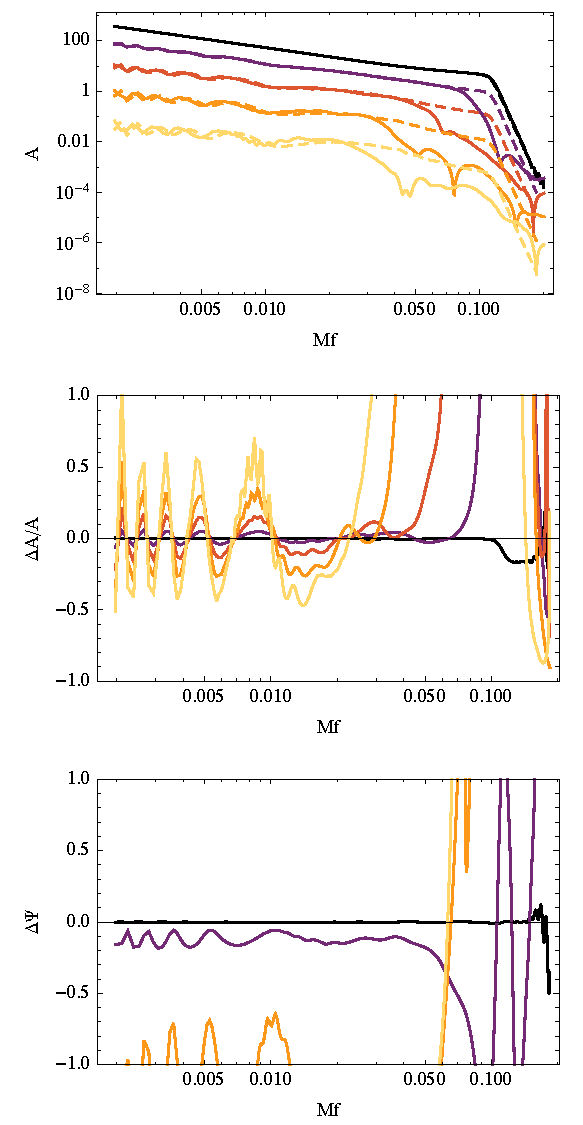
\includegraphics[width=.32\linewidth]{plots/precerrors_++_00_noconv_col.pdf}
  \hspace{0.cm}
  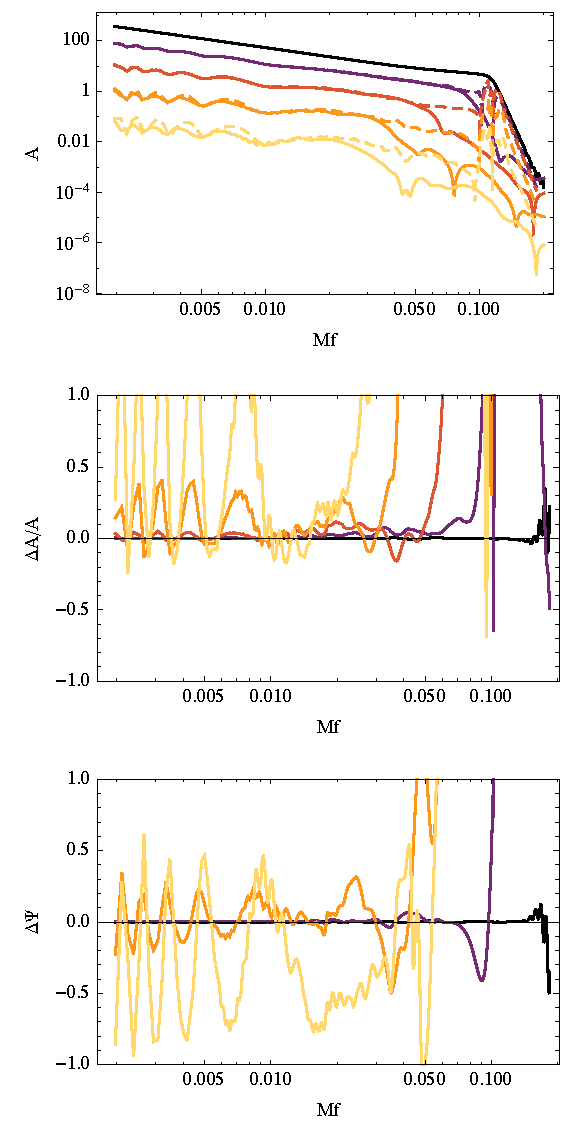
\includegraphics[width=.32\linewidth]{plots/precerrors_++_32_noconv_col.pdf}
  \hspace{0.cm}
  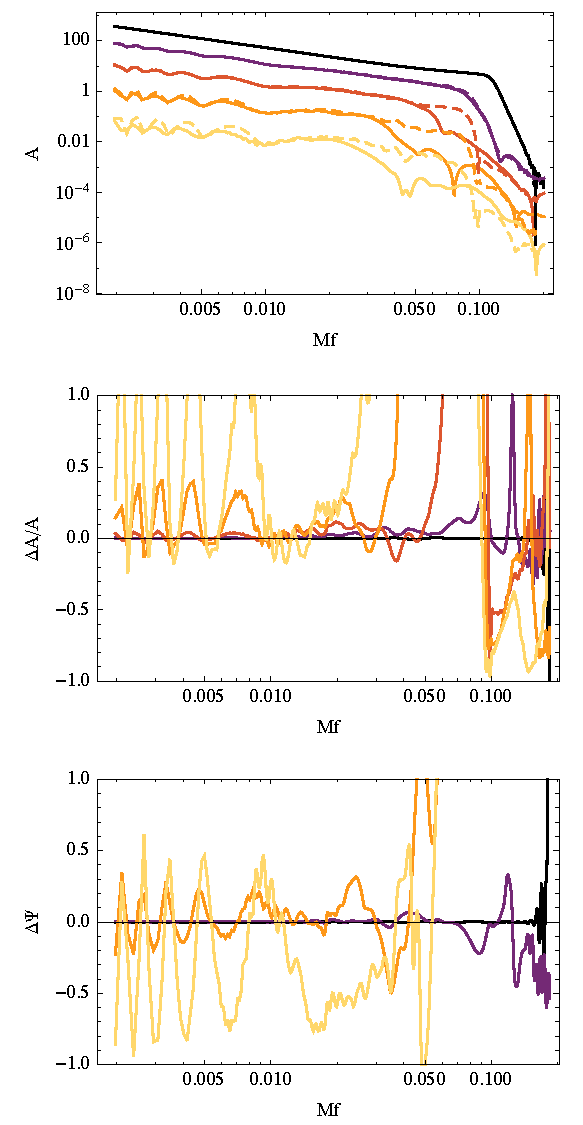
\includegraphics[width=.32\linewidth]{plots/precerrors_++_32_conv_col.pdf}
  \caption{Amplitude of the inertial-frame modes $h^{I}_{2m}$ and errors in the Fourier-domain transfer fonctions $\calT^{2}_{m2}$ for the configuration $++$. The columns show the orders of approximation $\{\Psi:0,A:0\}$, $\{\Psi:2,A:2\}$, $\{\Psi:2,A:2,\text{conv}\}$. \SM{[Compact the columns to share the x axis, add vertical line for merger frequency and shaded area for stitching pert/conv]} \SM{[check: where is the phase of the orange, mode 20 ?]}}
  \label{fig:precerrors++}
\end{figure*}

\begin{figure*}
  \centering
  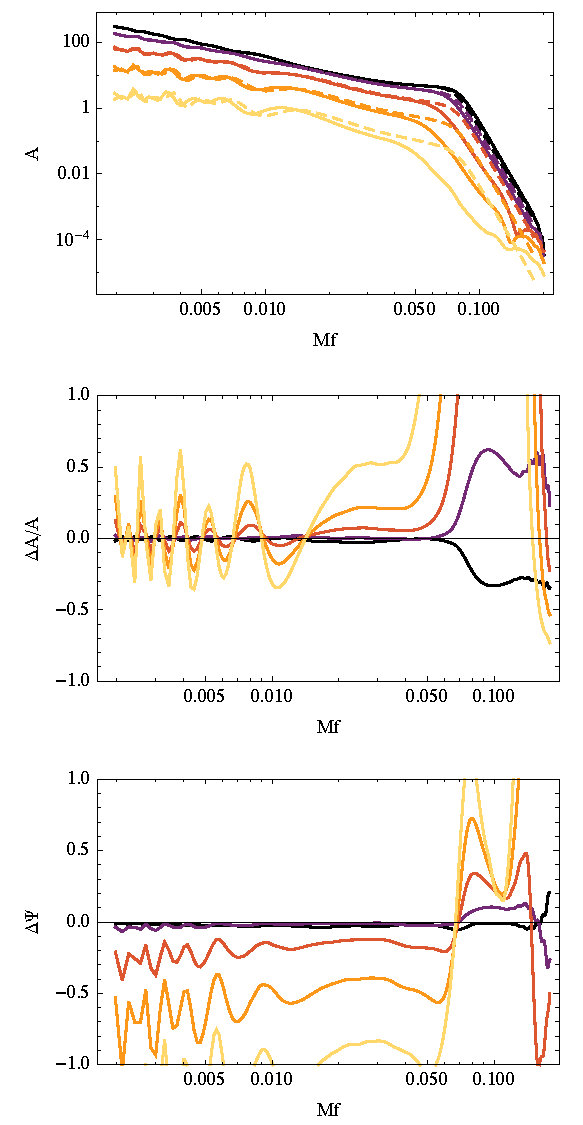
\includegraphics[width=.32\linewidth]{plots/precerrors_pp_00_noconv_col.pdf}
  \hspace{0.cm}
  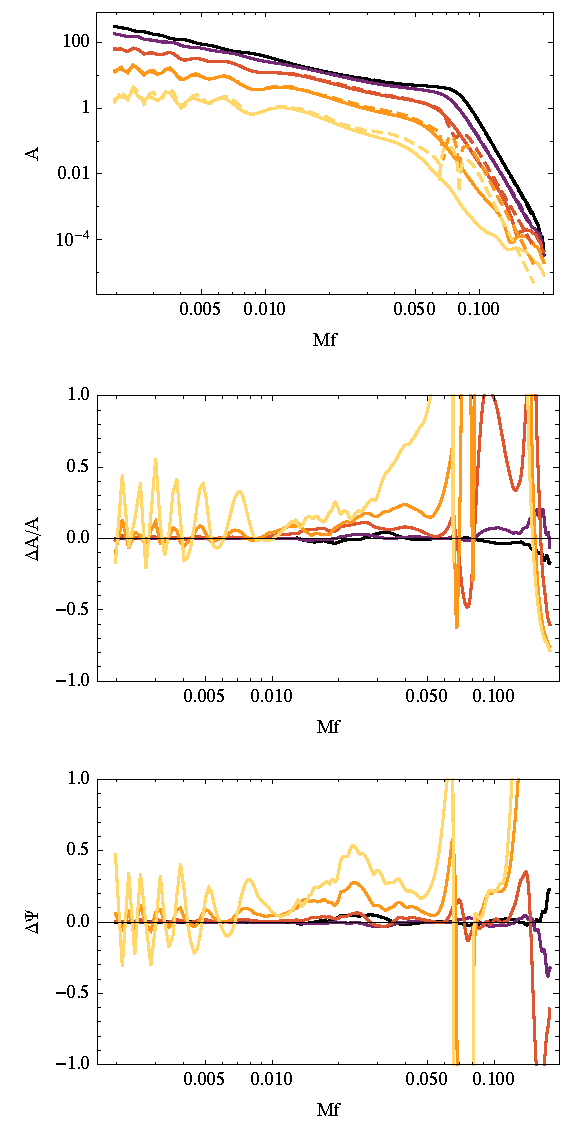
\includegraphics[width=.32\linewidth]{plots/precerrors_pp_32_noconv_col.pdf}
  \hspace{0.cm}
  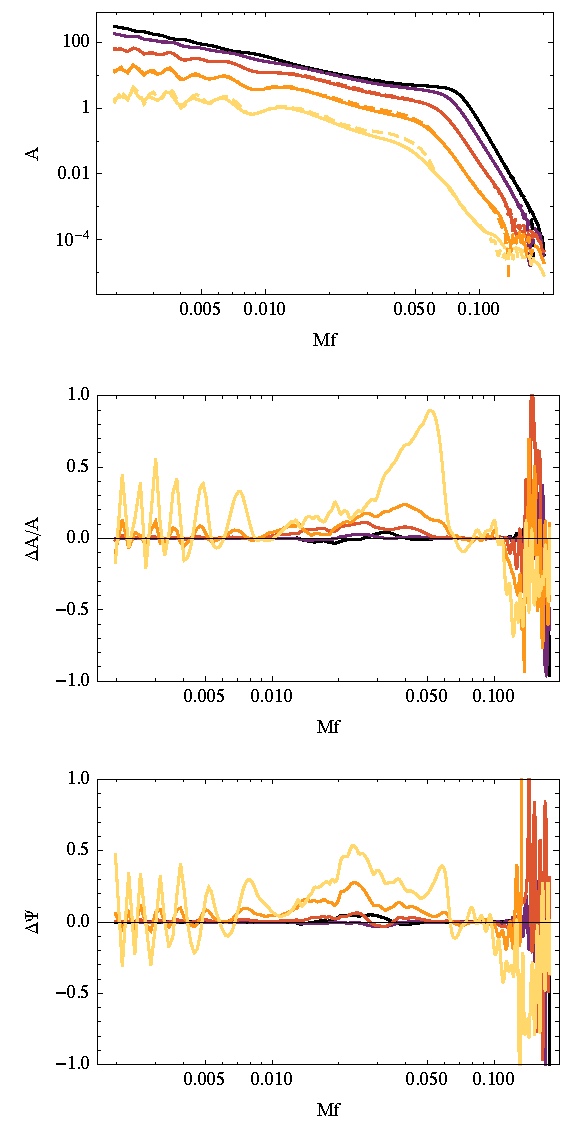
\includegraphics[width=.32\linewidth]{plots/precerrors_pp_32_conv_col.pdf}
  \caption{Amplitude of the inertial-frame modes $h^{I}_{2m}$ and errors in the Fourier-domain transfer fonctions $\calT^{2}_{m2}$ for the configuration $pp$. The columns show the orders of approximation $\{\Psi:0,A:0\}$, $\{\Psi:2,A:2\}$, $\{\Psi:2,A:2,\text{conv}\}$. \SM{[Compact the columns to share the x axis, add vertical line for merger frequency and shaded area for stitching pert/conv]}}
  \label{fig:precerrorspp}
\end{figure*}

\begin{figure*}
  \centering
  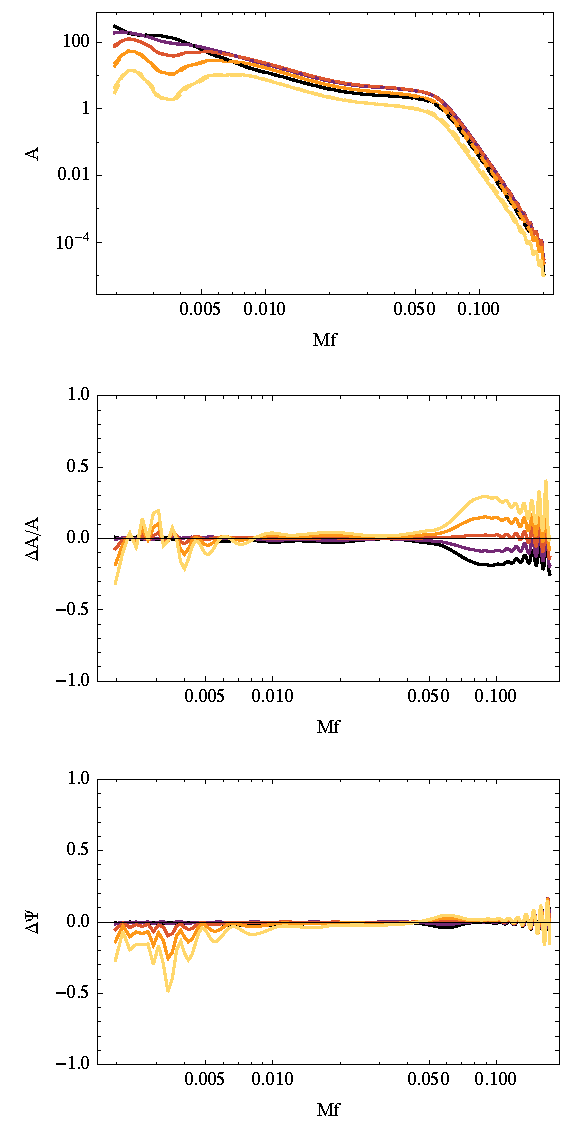
\includegraphics[width=.32\linewidth]{plots/precerrors_--_00_noconv_col.pdf}
  \hspace{0.cm}
  \includegraphics[width=.32\linewidth]{plots/precerrors_--_32_noconv_col.pdf}
  \hspace{0.cm}
  \includegraphics[width=.32\linewidth]{plots/precerrors_--_32_conv_col.pdf}
  \caption{Amplitude of the inertial-frame modes $h^{I}_{2m}$ and errors in the Fourier-domain transfer fonctions $\calT^{2}_{m2}$ for the configuration $--$. The columns show the orders of approximation $\{\Psi:0,A:0\}$, $\{\Psi:2,A:2\}$, $\{\Psi:2,A:2,\text{conv}\}$. \SM{[Compact the columns to share the x axis, add vertical line for merger frequency and shaded area for stitching pert/conv. Check the post-merger frame trajectory for - -.]}}
  \label{fig:precerrors--}
\end{figure*}

%\begin{figure*}
%  \centering
%  \includegraphics[width=.48\linewidth]{plots/precerrorA22caseI.pdf}
%  \hspace{0.2cm}
%  \includegraphics[width=.48\linewidth]{plots/precerrorPsi22caseI.pdf}
%  %
%  \includegraphics[width=.48\linewidth]{plots/precerrorA21caseI.pdf}
%  \hspace{0.2cm}
%  \includegraphics[width=.48\linewidth]{plots/precerrorPsi21caseI.pdf}  
%  \caption{Errors in the Fourier-domain transfer fonctions $\calT_{22,22}$ and $\calT_{22,21}$ as defined in~\eqref{eq:defTlmlmp}, for Case I and for various approximations. The black curve is the exact result provided by the FFT. The blue curve gives the leading-order, local approximation. The red curve includes quadratic corrections in phase and in amplitude. The yellow curve shows the result of the direct conolution approach of Sec.~\ref{subsec:directconvolution}. The left panels show the amplitude and the right panels the phase difference with the FFT. Note that the vertical scales are not uniform. [is it ok to show only 21 and 22 ? include the other modes which show problems ?]}
%  \label{fig:precerrorcaseI}
%\end{figure*}

%\begin{figure*}
%  \centering
%  \includegraphics[width=.48\linewidth]{plots/precerrorA22caseII.pdf}
%  \hspace{0.2cm}
%  \includegraphics[width=.48\linewidth]{plots/precerrorPsi22caseII.pdf}
%  %
%  \includegraphics[width=.48\linewidth]{plots/precerrorA21caseII.pdf}
%  \hspace{0.2cm}
%  \includegraphics[width=.48\linewidth]{plots/precerrorPsi21caseII.pdf}  
%  \caption{Errors in the Fourier-domain transfer fonctions $\calT_{22,22}$ and $\calT_{22,21}$. Conventions are the same as in Fig.~\ref{fig:precerrorcaseI} but for Case II, with a more rapid post-merger frame precession. Note that the vertical scales are not uniform. [is it ok to show only 21 and 22 ? include the other modes which show problems ?]}
%  \label{fig:precerrorcaseII}
%\end{figure*}

\SM{[say how the problems with reconstruction notably for ++ are probably caused by the convolution extending to the right and not to the left]}

%\begin{figure*}
%  \centering
%  \includegraphics[width=.48\linewidth]{plots/precmmsimple.pdf}
%  \hspace{0.2cm}
%  \includegraphics[width=.48\linewidth]{plots/precmmasympt.pdf}
%  \caption{Mismatches computed between the exact FFT and the various approximations respresented in Figs.~\ref{fig:precerrorcaseI} and~\ref{fig:precerrorcaseII}. [log scale for masses ? discuss the fact that in case II, leading order is accidentally better than Psi 2]}
%  \label{fig:precmm}
%\end{figure*}

\begin{figure*}
  \centering
  %
  \includegraphics[width=.32\linewidth]{plots/mismatches_++_inc0.pdf}
  \hspace{0.1cm}
  \includegraphics[width=.32\linewidth]{plots/mismatches_++_incpi3.pdf}
  \hspace{0.1cm}
  \includegraphics[width=.32\linewidth]{plots/mismatches_++_incpi2.pdf}
  %
  \includegraphics[width=.32\linewidth]{plots/mismatches_pp_inc0.pdf}
  \hspace{0.1cm}
  \includegraphics[width=.32\linewidth]{plots/mismatches_pp_incpi3.pdf}
  \hspace{0.1cm}
  \includegraphics[width=.32\linewidth]{plots/mismatches_pp_incpi2.pdf}
  %
  \includegraphics[width=.32\linewidth]{plots/mismatches_--_inc0.pdf}
  \hspace{0.1cm}
  \includegraphics[width=.32\linewidth]{plots/mismatches_--_incpi3.pdf}
  \hspace{0.1cm}
  \includegraphics[width=.32\linewidth]{plots/mismatches_--_incpi2.pdf}
  \caption{Unfaithfulness. Computed here with $f_{\rm min} = 20\mathrm{Hz}$, for masses between 20 and 400 $\Msol$, using the standard aLIGO noise curve \SM{[reference for that curve]}. \SM{[Extend computation to fmin=10 and Mmin=10]} \SM{[relate unfaithfulness levels to future detectors in the text]} }
  \label{fig:precunfaithfulness}
\end{figure*}

%%%%%%%%%%%%%%%%%%%%%%%%%%%%%%%%%%%%
%%%%%%%%%%%%%%%%%%%%%%%%%%%%%%%%%%%%

\section{Summary and Conclusions}
\label{sec:discussion}

[]

%%%%%%%%%%%%%%%%%%%%%%%%%%%%%%%%%%%%
%%%%%%%%%%%%%%%%%%%%%%%%%%%%%%%%%%%%

\vspace{4.5mm}

\hspace{0.85in}
{\bf Acknowledgments}

\vspace{3.5mm}

[Acknowledgments]

%%%%%%%%%%%%%%%%%%%%%%%%%%%%%%%%%%%%
%%%%%%%%%%%%%%%%%%%%%%%%%%%%%%%%%%%%

\appendix

\section{Notation and conventions}
\label{app:notation}

\SM{[add appendix with discrete Fourier coeffs]}

The convention we will be using for the Fourier transform of a signal $h(t)$ is
\be\label{eq:defFT}
	\tilde{h}(f) = \mathrm{FT}[h](f) =  \int \ud t \, e^{+2i\pi f t} h(t) \,.
\ee
Notice that this sign convention is not the most frequently used in the literature. We chose it to ensure that, with the conventions of~\cite{BlanchetLiving}, spin-weighted spherical modes $h_{\ell m}$ with $m>0$ will have support mostly for positive frequencies. One can revert to the more usual convention by taking $f\rightarrow -f$.

The effect of a shift in time of the time-domain signal translates into a linear phase contribution added to the Fourier-domain signal. For $h_{\Delta t}(t) \equiv h(t+\Delta t)$ with $\Delta t$ a constant, in our convention we have
\be\label{eq:shifttime}
	\tilde{h}_{\Delta t} (f) = e^{-2i\pi f \Delta t} \tilde{h}(f) \,.
\ee

A useful representation of the gravitational waveform is given by its decomposition in spin-weighted spherical harmonics. The waveform emitted in the direction $(\Theta, \Phi)$, with its two polarizations $h_{+},h_{\times}$, can be decomposed as a superposition of modes as~\cite{Thorne80}
\be\label{eq:defmodes}
	h_{+} - i h_{\times} = \sum\limits_{\ell \geq 2} \sum\limits_{m=-\ell}^{\ell} {}_{-2}Y_{\ell m}(\Theta,\Phi) h_{\ell m} \,,
\ee
where the ${}_{-2}Y_{\ell m}(\Theta,\Phi)$ are spin-weighted spherical harmonics~\cite{Goldberg+67}. Conversely, the individual polarizations are obtained from the individual modes as
\begin{subequations}
\begin{align}
	h_{+} = \frac{1}{2} \sum\limits_{\ell, m} \left[ {}_{-2}Y_{\ell m}h_{\ell m} + {}_{-2}Y_{\ell m}^{*} h_{\ell m}^{*} \right] \,,\\
	h_{\times} = \frac{i}{2} \sum\limits_{\ell, m} \left[ {}_{-2}Y_{\ell m}h_{\ell m} - {}_{-2}Y_{\ell m}^{*} h_{\ell m}^{*} \right] \,.
\end{align}
\end{subequations}

For a non-precessing system, with a fixed orbital plane, the individual modes have the additional symmetry property
\be\label{eq:symmetryhlminusm}
	h_{\ell, -m} = (-1)^{\ell} h_{\ell m}^{*} \,.
\ee
Since we will work in the Fourier domain, it will be useful to write the contributions of the individual modes to the Fourier transforms of the polarizations as
\begin{subequations}\label{eq:hpcfrommodes}
\begin{align}
	\tilde{h}_{+}(f) &= \frac{1}{2} \sum\limits_{\ell \geq 2} \sum\limits_{m=-\ell}^{\ell} \left[ {}_{-2}Y_{\ell m} \tilde{h}_{\ell m}(f) + {}_{-2}Y_{\ell m}^{*} \tilde{h}_{\ell m}(-f)^{*} \right] \,, \\
	\tilde{h}_{\times}(f) &= \frac{i}{2} \sum\limits_{\ell \geq 2} \sum\limits_{m=-\ell}^{\ell} \left[ {}_{-2}Y_{\ell m} \tilde{h}_{\ell m}(f) - {}_{-2}Y_{\ell m}^{*} \tilde{h}_{\ell m}(-f)^{*} \right] \,,
\end{align}
\end{subequations}
where we used $\widetilde{h_{\ell m}^{*}}(f) = \tilde{h}_{\ell m}(-f)^{*}$. An additional approximation often used in waveform models consists in considering that the Fourier transforms $\tilde{h}_{\ell m}$ have support only on one side of the spectrum, either for positive of for negative frequencies depending on the sign of $m$. This holds in particular within the stationary phase approximation, as explained below. With our sign convention~\eqref{eq:defFT}, this approximation reads
\begin{align}\label{eq:zeronegativef}
	\tilde{h}_{\ell m} (f) &\simeq 0 \text{ for } f<0, \; m>0 \nn\,,\\
	\tilde{h}_{\ell m} (f) &\simeq 0 \text{ for } f>0, \; m<0 \,.
\end{align}

In the following, we will drop the mode indices and the sum over modes, and we will denote generically by $h$ an individual mode of the waveform\footnote{This notation for a generic individual mode is not to be confused with the often encountered notation $h\equiv h_{+} - i h_{\times}$.}. Note that, if we are considering real signals $s(t)$ (such as $h_{+}$, $h_{\times}$, or any detector output), we can focus  on the positive-frequencies range and reconstruct the negative frequencies as $\tilde{s}(-f) = \tilde{s}(f)^{*}$. For positive frequencies $f>0$, we will use the generic notation $h$ as
\begin{align}\label{eq:notationhsignm}
	h(t) &\equiv h_{\ell m}(t) \,, \quad \tilde{h}(f) \equiv \tilde{h}_{\ell m}(f) \text{ for } m>0 \,, \nn\\
	h(t) &\equiv h_{\ell m}^{*}(t) \,, \quad \tilde{h}(f) \equiv \tilde{h}_{\ell m}(-f)^{*} \text{ for } m<0 \,.
\end{align}
We will further decompose $\tilde{h}$ into a Fourier-domain amplitude $A$ and a phase $\Psi$ according to
\be\label{eq:defAPsi}
	\tilde{h}(f) \equiv A(f) e^{-i\Psi(f)} \,.
\ee

Since we intend to work in the Fourier domain, we will use PhenomD waveforms~\cite{Khan+15}. These phenomenological waveforms provide analytic fits for both the Fourier-domain amplitude and phase of the 22 mode, with fit coefficients that were calibrated on EOB/NR hybrids [describe smoothing across intervals]. Fig.~\ref{fig:ampphase} shows an example of amplitude and phase in geometric units for an equal-mass binary.

%\begin{figure*}
%  \centering
%  \includegraphics[width=.48\linewidth]{plots/Af.pdf}
%  \hspace{0.2cm}
%  \includegraphics[width=.48\linewidth]{plots/Psif.pdf}
%  \caption{Fourier-domain amplitude and phase in geometric units for an equal-mass, non-spinning system. The vertical line represents $\omega_{22}^{\rm peak}/2\pi$, the frequency corresponding to the time-domain frequency of the waveform at the peak amplitude. The starting frequency $Mf_{min} = 2.6\times 10^{-4}$ is appropriate for a 2-years observation of a $M=10^{6} M_{\odot}$ system by LISA, or for an observation by LIGO/Virgo of a $M=5.4 M_{\odot}$ system entering the instrument band at $10\Hz$. [add residuals of interpolation on $~300$ points, to illustrate the compression of Amp/Phase FD waveforms ? or show different spins/mass ratios ?] \SM{[Plot perhaps not necessary ?]}}
%  \label{fig:ampphase}
%\end{figure*}

We recall that, with our sign convention, the effect of a positive shift in time $h' (t) = h(t- \Delta t)$ is
\be
	\tilde{h}'(f) = e^{2i\pi f \Delta t} \tilde{h}(f) \,.
\ee
If we also allow for a global shift in phase of the signal, which corresponds to a rotation of the unit vector pointing towards the observer in the frame of the gravitational waves source, a constant term can also be added (note that the effect of such a rotation gives different phase changes $e^{\pm i m \delta \phi}$ for the different modes of the radiation). We see that both a constant and a linear term in the Fourier-domain phase can be adjusted by changing extrinsic parameters. Thus, as is well known, apart from the relative phases of the modes for waveforms that include higher harmonics, the intrinsic information on the phasing is contained in the second derivative of the Fourier-domain phase $\Psi(f)$.

%%%%%%%%%%%%%%%%%%%%%%%%%%%%%%%%%%%%

\section{Wigner matrices and precessing frame}
\label{app:wigner}

In this Appendix, we summarize our conventions for the Wigner matrices.

\SM{[This differs from G. Faye's definition by a transposition $m\leftrightarrow m'$]}
\be\label{eq:defWignerDapp}
	\calD^{\ell}_{mm'} (\alpha, \beta, \gamma) = e^{im \alpha} d^{\ell}_{mm'}(\beta) e^{im' \gamma}\,,
\ee
\SM{[check]}
\begin{widetext}
\be\label{eq:defWignerdapp}
	d^{\ell}_{mm'}(\beta) = \sum\limits_{k=k_{\rm min}}^{k_{\rm max}} \frac{(-1)^{k}}{k!} \frac{\sqrt{(l+m)! (l-m)! (l+m')! (l-m')!}}{(l+m-k)! (l-m'-k)! (k-m+m')!} \left( \cos\frac{\beta}{2} \right)^{2\ell+m-m'-2k} \left( \sin\frac{\beta}{2} \right)^{2k-m+m'}\,,
\ee
\end{widetext}
where the boundaries of the sum, $k_{\rm min} = \mathrm{max}(0, m-m')$ and $k_{\rm max} = \mathrm{min}(\ell+m, \ell-m')$, can also be read by enforcing that the arguments of the factorials must be non-negative.

\SM{[add here explicitly the dominant-eigenvector construction of the P-frame]}


%%%%%%%%%%%%%%%%%%%%%%%%%%%%%%%%%%%%
%%%%%%%%%%%%%%%%%%%%%%%%%%%%%%%%%%%%

%\bibliography{ListeRef.bib}
\bibliography{references.bib}


\end{document}

